\documentclass[12pt,a4paper,violet]{bbe}
\usepackage{blindtext}

\usepackage[utf8]{inputenc} %Indica qué codificación se está usando ISO-8859-1(latin1)  o utf8  
\usepackage[spanish]{babel} %Indica que escribiermos en español   

                                                     
\usepackage{fancyhdr}                                        
\usepackage{amssymb}                                             
\usepackage{amsmath}
\usepackage{amsfonts}                                            
\usepackage{pdfpages}                                            
\usepackage{setspace}                                            
\usepackage{verbatim}
\usepackage{listings}    
%\usepackage[dvips]{graphicx}  
%\usepackage[hang,small,bf]{caption} % labelfont=bf
%\usepackage{caption} % labelfont=bf
%\captionsetup{skip=20pt,format=hang,font={color=ColorSecundario},labelfont=bf}

% Tablas
\usepackage{booktabs}                                          
\usepackage{multirow,array}
\usepackage{float}
%\usepackage{lscape}                                              
\usepackage{longtable}                               
\usepackage{pdfpages}



%...................
\renewcommand{\labelitemi}{$\bullet$}       
\renewcommand{\contentsname}{Contenido}                             
\renewcommand{\tablename}{Cuadro}                                 
\renewcommand{\listtablename}{Lista de Cuadros}                  
\renewcommand{\listfigurename}{Lista de Figuras}                  
%\renewcommand{\refname}{Bibliografía}

\decimalpoint                                                            

% Bibliografia
\usepackage{cite}
\usepackage{natbib}                
\usepackage{hyperref}  %elementos de los índices se vuelven clicables.                                          

\hypersetup{
             colorlinks,
             citecolor=blue,
             filecolor=blue,
             linkcolor=blue,
             urlcolor =blue
          } 

%%%%%%%%%%%%%%%%%%%%%%%%%%%%%%%%%%%%%%%
%--------- Documento
\begin{document}
\frontmatter     % Inicia numeración en romano
\thispagestyle{empty}
\hskip-1.5cm
%\begin{minipage}[c][0.05\height][c]{0.2\textwidth}
%\begin{center}
%    \includegraphics[width=2.5cm, height=3.5cm]{logo-uagro.pdf}
%\end{center}
%\end{minipage}
\hskip  0.6cm
\vspace{2pt}
\begin{minipage}[c][1\height][t]{0.83\linewidth}
\begin{flushleft}
    %{\scshape {\LARGE \textbf{Universidad  Aut\'onoma de Guerrero}}}\\
\end{flushleft}

%--- Línea horizontal
%\begin{center}
 %       \vspace{0.8cm}
   % {\Large Facultad de Matem\'aticas}
  %  \vspace{.4cm}
   % \hrule height2.3pt
%    \vspace{.1cm}
 %   \hrule height1pt
  %          \vspace{0.3cm}
    %{  \Large Maestr\'a en Matem\'aticas Aplicadas}

%\end{center}
\end{minipage}


\hskip-1.5cm

\begin{minipage}[c][0.7\textheight][t]{0.2\textwidth}
%----------   Línea vertical larga
%\begin{center}
%\vspace{15pt}
%\hskip1pt
%\vrule width 2.3 pt height 19cm
 %       \hskip2mm
  %      \vrule width1pt height19cm \\
        %\includegraphics[height=3cm]{logo-uagro.pdf}
 %       \end{center}
        
\end{minipage}\vspace{4 pt}
\thispagestyle{empty}
\hspace{0.5cm}

\begin{minipage}[c][0.7\textheight][t]{0.85\textwidth}
  \begin{center}
  \vspace{2cm}
    {\huge  \textbf{Modelos matemáticos para ciencias de datos}}

    \vspace{2cm}

%\textsc{\LARGE \bf T    E    S    I    S}\\[0.7cm]
%    PARA OBTENER EL GRADO DE:\\[10pt]
    {\Large \textbf{{María Guzmán Martínez \\Carlos David Carretillo Moctezuma}}}\\[40pt]
   % PRESENTA:\\[10pt]
  %  \Large \textbf{{Nombre}}

  %  \vspace{1cm}

%   {\normalsize Dra. María Guzmán Martínez:}\\[2pt] 

   % \vspace{1.5cm}
  \end{center}
   
\begin{flushright}
    {\large abril,  2024.}
 \end{flushright}
 
\end{minipage}   % PortadaUAGRO archivo .TEx


% Se agragan en el índice
% Índice de contenido
\addcontentsline{toc}{chapter}{Índice general}
\tableofcontents

% Índice de tablas
%\addcontentsline{toc}{chapter}{Índice de tablas}  % Nombre
%\listoftables

% Índice de figuras
\addcontentsline{toc}{chapter}{Índice de figuras}
\listoffigures

%\maketitle

\mainmatter % Se da inicio al cuerpo del documento; se numeran los capítulos y las páginas con números arábigos 

\chapter{Álgebra de matrices y vectores}

%%%%%%%%%%%%%%%%%%%%%%%%%%%%%%%%%%%%%%%%%%%%%%%%%%%
\section{Vectores} 

%\textcolor{red}{Carlos, para la redacción de este capítulo apóyese del Johnson. capítulo 2: Matrix Algebra and Random Vectors}
\begin{definition}[Vector]
Un vector $\boldsymbol{V}$ en el plano $xy$ es un par ordenado de números reales $(a, b)$. Los números $a$ y $b$ se denominan elementos o componentes del vector $\boldsymbol{V}$. El vector cero es el vector $(0, 0)$.

\end{definition}
\begin{definition}
Un conjunto $x$ de $n$ números reales $x_1, x_2, \ldots, x_n$ se llama un vector, y se escribe como:\\
  \[
\boldsymbol{A} = \begin{pmatrix}
x_1 \\
x_2 \\
\vdots \\
x_n
\end{pmatrix}
\quad
\text{ó}
\quad
\boldsymbol{A}^\top = [x_1, x_2, \ldots, x_n]
\]

\end{definition}
\begin{definition}
Un vector fila de $n$ componentes se define como un conjunto ordenado de $n$ números escritos de la siguiente manera: $$(x_1, x_2, \ldots, x_n)$$.    
\end{definition}
\begin{definition}
Un vector columna de $n$ componentes es un conjunto ordenado de $n$ números escritos de la siguiente manera:
\[
\begin{pmatrix}
x_1 \\
x_2 \\
\vdots \\
x_n
\end{pmatrix}
\]  
\end{definition}
A continuación se muestran las propiedades de los vectores:\\

\begin{enumerate}
    \item  \text{Suma de vectores:} $\quad \mathbf{V} + \mathbf{W} = \mathbf{W} + \mathbf{V} $\\
\item  \text{Multiplicación por un escalar:} $\quad c(\mathbf{V} + \mathbf{W}) = c\mathbf{V} + c\mathbf{W}$ \\
\item  \text{Distributiva de la suma de escalares:} $\quad (a + b)\mathbf{V} = a\mathbf{V} + b\mathbf{V}$ \\
\item  \text{Producto punto:}$ \quad \mathbf{u} \cdot \mathbf{V} = \sum_{i=1}^{n} u_iv_i $\\
\item  \text{Producto cruz:} $\quad \mathbf{V} \times \mathbf{W} = \begin{pmatrix} v_2 w_3 - v_3 w_2 \\ v_3 w_1 - v_1 w_3 \\ v_1 w_2 - v_2 w_1 \end{pmatrix} $\\
\item  \text{Norma o módulo de un vector:} $\quad \|\mathbf{V}\| = \sqrt{v_1^2 + v_2^2 + \ldots + v_n^2}$ \\
\item   \text{Vectores ortogonales:} $\quad \mathbf{V} \perp \mathbf{W} \quad \text{si} \quad \mathbf{V} \cdot \mathbf{W} = 0$
\end{enumerate}


%----------------------------------------------
\subsection{Resolución de problemas}

%----------------------------------------------
\begin{example}
   La suma de dos vectores en un espacio euclidiano se realiza sumando componente por componente. Si tienes dos vectores $\mathbf{U}$ y $\mathbf{V}$ dados por:

\[
\boldsymbol{U} = \begin{pmatrix} u_1 \\ u_2 \\ \vdots \\ u_n \end{pmatrix} \quad \text{y} \quad \boldsymbol{V} = \begin{pmatrix} v_1 \\ v_2 \\ \vdots \\ v_n \end{pmatrix}
\]

entonces la suma de estos vectores, denotada como $\mathbf{U} + \mathbf{V}$, se calcula sumando sus componentes correspondientes:

\[
\boldsymbol{U} + \boldsymbol{V} = \begin{pmatrix} u_1 + v_1 \\ u_2 + v_2 \\ \vdots \\ u_n + v_n \end{pmatrix}
\]
\end{example}
\begin{example}
    Consideremos dos vectores en \( \mathbb{R}^3 \):
\[
\boldsymbol{U} = \begin{pmatrix} 2 \\ -1 \\ 3 \end{pmatrix} \quad \text{y} \quad \boldsymbol{V} = \begin{pmatrix} -3 \\ 2 \\ 1 \end{pmatrix}
\]

La suma de estos vectores es:
\[
\boldsymbol{U} + \boldsymbol{V} = \begin{pmatrix} 2 \\ -1 \\ 3 \end{pmatrix} + \begin{pmatrix} -3 \\ 2 \\ 1 \end{pmatrix} = \begin{pmatrix} 2 + (-3) \\ (-1) + 2 \\ 3 + 1 \end{pmatrix} = \begin{pmatrix} -1 \\ 1 \\ 4 \end{pmatrix}
\]
\end{example}
%%%%%%%%%%%%%%%%%%%%%%%%%%%
\begin{example}
    Consideremos dos vectores \( \mathbf{U} = \begin{pmatrix} 3 \\ -1 \\ 2 \end{pmatrix} \) y \( \mathbf{V} = \begin{pmatrix} -2 \\ 4 \\ 1 \end{pmatrix} \). La resta de \( \mathbf{U} \) por \( \mathbf{V} \) es:

\[
\boldsymbol{U} - \boldsymbol{V} = \begin{pmatrix} 3 \\ -1 \\ 2 \end{pmatrix} - \begin{pmatrix} -2 \\ 4 \\ 1 \end{pmatrix} = \begin{pmatrix} 3 - (-2) \\ -1 - 4 \\ 2 - 1 \end{pmatrix} = \begin{pmatrix} 5 \\ -5 \\ 1 \end{pmatrix}
\]
\end{example}
%%%%%%%%%%%%%%%%%%%%%%%%%%%%%%
\begin{exercise}
Dado el vector \( \mathbf{V} = \begin{pmatrix} 3 \\ -2 \\ 5 \end{pmatrix} \) y el vector \( \mathbf{U} = \begin{pmatrix} -1 \\ 4 \\ 2 \end{pmatrix} \), calcula \( \mathbf{V} + \mathbf{U} \).
\end{exercise}
%%%%%%%%%%%%%%%%%%%%%%%%%%%%%%%%%%
\begin{exercise}
Sean \( \mathbf{A} = \begin{pmatrix} 2 \\ 1 \end{pmatrix} \) y \( \mathbf{B} = \begin{pmatrix} -3 \\ 5 \end{pmatrix} \) dos vectores en \( \mathbb{R}^2 \). Calcula \( \mathbf{A} - \mathbf{B} \).
\end{exercise}
\subsection{Practica con R}
\begin{verbatim}
%%%%%%%%%%%%%%%%%%%%%%%%%%%%%%%%%%%%%%%%%%%%%%%%%%%%%%%%%%%%%%%%%%
  # Definir dos vectores
v1 <- c(1, 2, 3)
v2 <- c(4, 5, 6)

# Sumar los vectores
suma <- v1 + v2

# Mostrar el resultado
print(suma)  
%%%%%%%%%%%%%%%%%%%%%%%%%%%%%%%%%%%%%%%%%%%%%%%%%%%%%%%%%%%%%%%%%
\end{verbatim}
\begin{verbatim}
 # Definir los vectores columna
U <- c(1, 2, 3)
V <- c(4, 5, 6)

# Calcular la resta de los vectores
resultado <- U - V

# Mostrar el resultado
print("Resultado de la resta de los vectores:")
print(resultado)  
%%%%%%%%%%%%%%%%%%%%%%%%%%%%%%%%%%%%%%%%%%%%%%%%%%%%%%%%%%%%%%%%%%
\end{verbatim}
\begin{verbatim}
# Definir un vector de lógicos y un vector de enteros
v_logico <- c(TRUE, FALSE, TRUE)
v_entero <- c(1, 0, 1)

# Sumar los vectores
suma <- v_logico + v_entero

# Mostrar el resultado
print(suma)
%%%%%%%%%%%%%%%%%%%%%%%%%%%%%%%%%%%%%%%%%%%%%%%%%%%%%%%%%%%%%%%%%%
\end{verbatim}
%%%%%%%%%%%%%%%%%%%%%%%%%%%%%%%%%
\begin{definition}
Sea \( \mathbf{V} = \begin{pmatrix} v_1 \\ v_2 \\ \vdots \\ v_n \end{pmatrix} \) un vector en \( \mathbb{R}^n \) y \( k \) un escalar. La multiplicación de \( \mathbf{V} \) por \( k \) se calcula como:

\[
k \boldsymbol{V} = k \begin{pmatrix} v_1 \\ v_2 \\ \vdots \\ v_n \end{pmatrix} = \begin{pmatrix} k v_1 \\ k v_2 \\ \vdots \\ k v_n \end{pmatrix}
\]
\end{definition}
%%%%%%%%%%%%%%%%%%%%%%%%%%%%%%%%%%
\begin{example}
Sea el vector \( \mathbf{V} = \begin{pmatrix} 2 \\ -3 \\ 1 \end{pmatrix} \) y el escalar \( k = 3 \). La multiplicación de \( \mathbf{V} \) por \( k \) es:

\[
k \boldsymbol{V} = 3 \begin{pmatrix} 2 \\ -3 \\ 1 \end{pmatrix} = \begin{pmatrix} 3 \cdot 2 \\ 3 \cdot (-3) \\ 3 \cdot 1 \end{pmatrix} = \begin{pmatrix} 6 \\ -9 \\ 3 \end{pmatrix}
\]
\end{example}
%%%%%%%%%%%%%%%%%%%%%%%%%%
\begin{example}
    Consideremos el vector fila \( \mathbf{V} = (1, 2, 3) \) y el escalar \( k = 2 \). La multiplicación de \( \mathbf{V} \) por \( k \) es:

\[
k \boldsymbol{V} = 2 (1, 2, 3) = (2 \cdot 1, 2 \cdot 2, 2 \cdot 3) = (2, 4, 6)
\]

\end{example}
%%%%%%%%%%%%%%%%%%%%%%%%%
\begin{exercise}
 Sea $\mathbf{A}=\left(\begin{array}{l}4 \\ 6 \\ 1 \\ 3\end{array}\right) \quad y \quad \mathbf{B}=\left(\begin{array}{r}-2 \\ 4 \\ -3 \\ 0\end{array}\right)$. Calcule $2 \mathbf{A}-3 \mathbf{B}$.   
\end{exercise}
\begin{solution}
     Solución $2 \mathbf{A}-3 \mathbf{B}=2\left(\begin{array}{l}4 \\ 6 \\ 1 \\ 3\end{array}\right)+(-3)\left(\begin{array}{r}-2 \\ 4 \\ -3 \\ 0\end{array}\right)=\left(\begin{array}{r}8 \\ 12 \\ 2 \\ 6\end{array}\right)+\left(\begin{array}{r}6 \\ -12 \\ 9 \\ 0\end{array}\right)=\left(\begin{array}{r}14 \\ 0 \\ 11 \\ 6\end{array}\right)$
\end{solution}

%%%%%%%%%%%%%%%%%%%%%%%%%%
\begin{exercise}
Dado el vector \( \mathbf{W} = \begin{pmatrix} -1 \\ 3 \\ 0 \end{pmatrix} \), encuentra \( \frac{1}{2} \mathbf{W} \).
\end{exercise}

\begin{exercise}
Sean \( \mathbf{C} = \begin{pmatrix} 1 \\ 0 \\ -2 \end{pmatrix} \) y \( \mathbf{D} = \begin{pmatrix} 4 \\ -3 \\ 1 \end{pmatrix} \) dos vectores en \( \mathbb{R}^3 \). Calcula el producto escalar \( \mathbf{C} \cdot \mathbf{D} \).
\end{exercise}
\subsection{Práctica con R}
Los vectores de datos $x$ y $y$, se pueden concatenar por columnas con la función  \textit{cbind()}; y  por renglones con
la función \textit{rbind()}.
\begin{verbatim}
%%%%%%%%%%%%%%%%%%%%%%%%%%%%%%%%%%%%%%%%%%%%%%%%%%%%%%%%%%%%%%%%%%%%
# Los vectores de datos $x$ y $y$, Por renglones (filas)
      A<-rbind(x, y)
      A
# La función \textit{matrix()} genera una matriz; el número de columnas y 
renglones (filas) de la matriz se indican con los argumentos \textit{ncol}
y\textbf{nrow}, respectivamente.
      x <- c(2, 7, 3, 6, 1)
      y <- c(3, 7, 3, 5, 9)

      # Creando la matriz
      A<-matrix(c(x,y), nrow = 5, ncol = 2)
      A
#La dimensión de la matriz $A$, está dada por:
       dim(A)
# Usando \texttt{byrow = TRUE}: Esto indica que los elementos de la matriz 
se llenarán por filas. Es decir, la primera fila se llenará primero, luego
la segunda fila y así sucesivamente.

# Usando \texttt{ncol =}: Esto indica el número de columnas de la matriz. 
Si utilizas \texttt{ncol =} en lugar de \texttt{byrow = TRUE}, se llenará 
la matriz por columnas en lugar de por filas.

# Para determinar de qué clase es el objeto que se definió se usa la función
\textit{class()}:
      class(A)

Dimensión de la matriz $A$: 
      dim(A) 

      x <- c(2, 7, 3, 6, 1)
      y <- c(3, 7, 3, 5, 9)

      # Por columnas
      A<-cbind(x, y)
      A
%%%%%%%%%%%%%%%%%%%%%%%%%%%%%%%%%%%%%%%%%%%%%%%%%%%%%%%%%%%%%%%%%%%%
\end{verbatim}
\begin{verbatim}
# Definir la matriz original
A <- matrix(c(1, 2, 3, 4, 5, 6), nrow = 2, byrow = TRUE)
print("Matriz original:")
print(A)

# Definir el escalar
escalar <- 3

# Multiplicar la matriz por el escalar
resultado <- escalar * A

# Mostrar el resultado
print("Matriz resultante después de la multiplicación por el escalar:")
print(resultado)
%%%%%%%%%%%%%%%%%%%%%%%%%%%%%%%%%%%%%%%%%%%%%%%%%%%%%%%%%%%%%%%%%%%%
\end{verbatim}
\begin{verbatim}
# Definir los vectores A y B
A <- c(1, 2, 3)
B <- c(4, 5, 6)

# Definir el escalar fraccionado y el escalar entero
escalar_fraccionado <- 3/2
escalar_entero <- 2

# Calcular la operación
resultado <- escalar_fraccionado * A - escalar_entero * B

# Mostrar el resultado
print("Resultado de la operación:")
print(resultado)
%%%%%%%%%%%%%%%%%%%%%%%%%%%%%%%%%%%%%%%%%%%%%%%%%%%%%%%%%%%%%%%%%%%%    
\end{verbatim}
%%%%%%%%%%%%%%%%%%%%%%%%
\begin{definition}
El producto punto o producto escalar de dos vectores $\mathbf{U} = (u_1, u_2, u_3)$ y $\mathbf{V} = (v_1, v_2, v_3)$ se denota como $\mathbf{U} \cdot \mathbf{V}$.
    \[
\boldsymbol{U} \cdot \boldsymbol{V} = u_1 v_1 + u_2 v_2 + u_3 v_3
\]
Dado el vector fila \( \mathbf{U} = [u_1, u_2, u_3] \) y el vector columna \( \mathbf{V} = \begin{pmatrix} v_1 \\ v_2 \\ v_3 \end{pmatrix} \), el producto escalar \( \mathbf{U} \cdot \mathbf{V} \) se calcula como:

\[
\boldsymbol{U} \cdot \boldsymbol{V} = [u_1, u_2, u_3] \begin{pmatrix} v_1 \\ v_2 \\ v_3 \end{pmatrix} = u_1 v_1 + u_2 v_2 + u_3 v_3
\]
\end{definition}
%%%%%%%%%%%%%%%%%%%%%
\begin{example}
Sea el vector fila \( \mathbf{U} = [1, 2, 3] \) y el vector columna \( \mathbf{V} = \begin{pmatrix} 4 \\ 5 \\ 6 \end{pmatrix} \). El producto escalar \( \mathbf{U} \cdot \mathbf{V} \) se calcula como:

\[
\boldsymbol{U} \cdot \boldsymbol{V} = [1, 2, 3] \begin{pmatrix} 4 \\ 5 \\ 6 \end{pmatrix} = 1 \cdot 4 + 2 \cdot 5 + 3 \cdot 6 = 4 + 10 + 18 = 32
\]    
\end{example}
%%%%%%%%%%%%%%%%%%%%
\begin{example}
Supongamos el vector fila \( \mathbf{A} = [2, -1, 3] \) y el vector columna \( \mathbf{B} = \begin{pmatrix} -1 \\ 2 \\ 4 \end{pmatrix} \). El producto escalar \( \mathbf{A} \cdot \mathbf{B} \) se obtiene como:

\[
\mathbf{A} \cdot \mathbf{B} = [2, -1, 3] \begin{pmatrix} -1 \\ 2 \\ 4 \end{pmatrix} = 2 \cdot (-1) + (-1) \cdot 2 + 3 \cdot 4 = -2 - 2 + 12 = 8
\]

\end{example}
%%%%%%%%%%%%%%%%%%%
\begin{tcolorbox}[colback=white!5!white,colframe=red!50!red,title=Teorema]
Sean $\mathbf{A}$, $\mathbf{B}$ y $\mathbf{C}$ tres vectores de dimensión \(n\) y sea \(a\) un escalar. Entonces:
\begin{enumerate}
    \item \( \mathbf{A} \cdot \mathbf{0} = 0 \)
    \item \( \mathbf{A} \cdot \mathbf{B} = \mathbf{B} \cdot \mathbf{A} \) (ley conmutativa del producto escalar)
    \item \( \mathbf{A} \cdot (\mathbf{B} + \mathbf{C}) = \mathbf{A} \cdot \mathbf{B} + \mathbf{A} \cdot \mathbf{C} \) (ley distributiva del producto escalar)
    \item \( (\alpha \cdot \mathbf{A}) \cdot \mathbf{B} = \alpha \cdot (\mathbf{A} \cdot \mathbf{B}) \)
\end{enumerate}
\end{tcolorbox}
\begin{remark}
Observe que no existe una ley asociativa para el producto escalar. La expresión $(A\cdot B) \cdot C =
A\cdot(B\cdot C) $ no tiene sentido porque ninguno de los dos lados de la ecuación está definido.   
\end{remark}
\begin{exercise}
 Dado el vector fila \( \mathbf{A} = [\mathbf{1}, \mathbf{-2}, \mathbf{3}] \) y el vector columna \( \mathbf{B} = \begin{pmatrix} \mathbf{4} \\ \mathbf{5} \\ \mathbf{6} \end{pmatrix} \), calcular \( \mathbf{A} \cdot \mathbf{B} \)  
\end{exercise}

\begin{exercise}
Sean \( \mathbf{U} = [\mathbf{2}, \mathbf{1}, \mathbf{-3}] \) y \( \mathbf{V} = \begin{pmatrix} \mathbf{-1} \\ \mathbf{0} \\ \mathbf{2} \end{pmatrix} \) dos vectores. Encuentra \( \mathbf{U} \cdot \mathbf{V} \) 
\end{exercise}
\begin{exercise}
Dado el vector fila \( \mathbf{X} = [\mathbf{1}, \mathbf{2}] \) y el vector columna \( \mathbf{Y} = \begin{pmatrix} \mathbf{-3} \\ \mathbf{4} \end{pmatrix} \), calcular \( \mathbf{X} \cdot \mathbf{Y} \)  
\end{exercise}
\subsection{Práctica con R}
\begin{verbatim}
%%%%%%%%%%%%%%%%%%%%%%%%%%%%%%%%%%%%%%%%%%%%%%%%%%%%%%%%%%%%%%%%%%%%%%%
 # Definir los vectores
v1 <- c(1, 2, 3)
v2 <- c(4, 5, 6)

# Calcular el producto punto
producto_punto <- sum(v1 * v2)

# Mostrar el resultado
print(paste("El producto punto de", v1, "y", v2, "es:", producto_punto))  
%%%%%%%%%%%%%%%%%%%%%%%%%%%%%%%%%%%%%%%%%%%%%%%%%%%%%%%%%%%%%%%%%%%%%%%
\end{verbatim}
\begin{verbatim}

# Definir un vector columna y un vector fila
vector_columna <- matrix(c(1, 2, 3), ncol = 1)
vector_fila <- c(4, 5, 6)

# Calcular el producto punto
producto_punto <- sum(vector_columna * vector_fila)

# Mostrar el resultado
print(paste("El producto punto entre el vector columna y el vector fila es:
", producto_punto))    
%%%%%%%%%%%%%%%%%%%%%%%%%%%%%%%%%%%%%%%%%%%%%%%%%%%%%%%%%%%%%%%%%%%%%%%
\end{verbatim}
\begin{verbatim}
# Definir dos vectores
u <- c(1, 2, 3)
v <- c(4, 5, 6)

# Definir un escalar
c <- 2

# Calcular el producto escalar del lado izquierdo de la ecuación
izquierda <- c * (u + v)

# Calcular el producto escalar del lado derecho de la ecuación
derecha <- c * u + c * v

# Mostrar los resultados
print("Lado izquierdo de la ecuación:")
print(izquierda)
print("Lado derecho de la ecuación:")
print(derecha)

# Comprobar si los resultados son iguales
if(all.equal(izquierda, derecha)) {
  print("La ley distributiva del producto escalar se cumple.")
} else {
  print("La ley distributiva del producto escalar NO se cumple.")
}
%%%%%%%%%%%%%%%%%%%%%%%%%%%%%%%%%%%%%%%%%%%%%%%%%%%%%%%%%%%%%%%%%%%%%%%    
\end{verbatim}
\begin{verbatim}
    # Definir tres vectores
A <- c(1, 2, 3)
B <- c(4, 5, 6)
C <- c(7, 8, 9)

# Calcular el lado izquierdo de la ecuación
lado_izquierdo <- sum(A * (B + C))

# Calcular el lado derecho de la ecuación
lado_derecho <- sum(A * B) + sum(A * C)

# Mostrar los resultados
print("Lado izquierdo de la ecuación:")
print(lado_izquierdo)
print("Lado derecho de la ecuación:")
print(lado_derecho)

# Comprobar si los resultados son iguales
if(lado_izquierdo == lado_derecho) {
  print("La ley distributiva del producto escalar se cumple.")
} else {
  print("La ley distributiva del producto escalar NO se cumple.")
}
%%%%%%%%%%%%%%%%%%%%%%%%%%%%%%%%%%%%%%%%%%%%%%%%%%%%%%%%%%%%%%%%%%%%%%%
\end{verbatim}
%%%%%%%%%%%%%%%%%%%%5
\begin{definition}
Dados los vectores $\mathbf{U} = (a, b, c)$ y $\mathbf{V} = (a_1, b_1, c_1)$, se define el producto cruz o producto vectorial de $\mathbf{U}$ y $\mathbf{V}$ como $\mathbf{U} \times \mathbf{V}$:=$(bc_1 - b_1 c, a_1 c - a c_1, ab_1 - a_1 b)$.    
\end{definition}

Algunas propiedades del producto cruz se muestran a continuación.
\begin{itemize}
   
\item \textbf{Anticonmutatividad}: $\mathbf{u} \times \mathbf{v} =-(\mathbf{v} \times \mathbf{u})$.

\item \textbf{Distributividad con respecto a la suma}: $\mathbf{u} \times (\mathbf{v} + \mathbf{w}) = \mathbf{u} \times \mathbf{v} + \mathbf{u} \times \mathbf{w}$.

\item \textbf{No es asociativo}: $(\mathbf{u} \times \mathbf{v}) \times \mathbf{w} \neq \mathbf{u} \times (\mathbf{v} \times \mathbf{w})$.

\item \textbf{El producto cruz de dos vectores paralelos es cero}: Si $\mathbf{u}$ y $\mathbf{v}$ son paralelos o antiparalelos, entonces $\mathbf{u} \times \mathbf{v} = \mathbf{0}$.

\end{itemize}
%%%%%%%%%%%%%%%%%%%%%%%%%%%%%
\begin{example}
Dados los vectores $\mathbf{U} = \begin{pmatrix} \boldsymbol{2} \\ \boldsymbol{-1} \\ \boldsymbol{3} \end{pmatrix}$ y $\mathbf{V} = \begin{pmatrix} \boldsymbol{1} \\ \boldsymbol{4} \\ \boldsymbol{-2} \end{pmatrix}$, demostraremos la propiedad de anticonmutatividad del producto cruz.

Calculamos $\mathbf{U} \times \mathbf{V}$:
\[
\mathbf{U} \times \mathbf{V} = \begin{pmatrix} -1( -2 ) - 3( 4 ) \\ 3( 1 ) - 2( -2 ) \\ 2( 4 ) - (-1)( 1 ) \end{pmatrix} = \begin{pmatrix} -10 \\ 7 \\ 9 \end{pmatrix}
\]

Ahora calculamos $\mathbf{V} \times \mathbf{U}$:
\[ \begin{pmatrix}
(4 \times 3) - (-2 \times (-1)) \\
(-2 \times 2) - (1 \times 3) \\
(1 \times (-1)) - (4 \times 2)
\end{pmatrix} = \begin{pmatrix} 10 \\ -7 \\ -9 \end{pmatrix}
\]

Como $\mathbf{U} \times \mathbf{V} = \begin{pmatrix} -10 \\ 7 \\ 9 \end{pmatrix}$ y $\mathbf{V} \times \mathbf{U} = \begin{pmatrix} 10 \\ -7 \\ -9 \end{pmatrix}$ son opuestos, se cumple la propiedad de anticonmutatividad.

\end{example}
%%%%%%%%%%%%%%%%%%%%
\begin{example}
Dados los vectores $\mathbf{U} = \begin{pmatrix} \boldsymbol{2} \\ \boldsymbol{1} \\ \boldsymbol{-3} \end{pmatrix}$, $\mathbf{V} = \begin{pmatrix} \boldsymbol{-1} \\ \boldsymbol{0} \\ \boldsymbol{2} \end{pmatrix}$ y $\mathbf{W} = \begin{pmatrix} \boldsymbol{3} \\ \boldsymbol{4} \\ \boldsymbol{-1} \end{pmatrix}$, demostraremos la propiedad de distributividad con respecto a la suma del producto cruz.

Calculamos $\mathbf{U} \times (\mathbf{V} + \mathbf{W})$:
\[
\mathbf{U} \times (\mathbf{V} + \mathbf{W}) = \mathbf{U} \times \begin{pmatrix} -1+3 \\ 0+4 \\ 2-1 \end{pmatrix} = \mathbf{U} \times \begin{pmatrix} \boldsymbol{2} \\ \boldsymbol{4} \\ \boldsymbol{1} \end{pmatrix} = \begin{pmatrix} (1)(1) - (-3)(4) \\ (-3)(2) - (2)(1) \\ (2)(4) - (1)(1) \end{pmatrix} = \begin{pmatrix} 13 \\ -8 \\ 7 \end{pmatrix}
\]

Ahora calculamos $\mathbf{U} \times \mathbf{V} + \mathbf{U} \times \mathbf{W}$:
\[
\mathbf{U} \times \mathbf{V} + \mathbf{U} \times \mathbf{W} = \begin{pmatrix} (1)(0) - (-3)(2) \\ (-3)(-1) - (2)(3) \\ (2)(4) - (1)(-1) \end{pmatrix} + \begin{pmatrix} (1)(4) - (-3)(-1) \\ (-3)(3) - (2)(-3) \\ (2)(-1) - (1)(4) \end{pmatrix} = \begin{pmatrix} 6 \\ -13 \\ 9 \end{pmatrix} + \begin{pmatrix} 7 \\ -5 \\ -6 \end{pmatrix} = \begin{pmatrix} 13 \\ -8 \\ 7 \end{pmatrix}\]
\end{example}
\begin{exercise}
 Demostrar que : $(\mathbf{u} \times \mathbf{v}) \times \mathbf{w} \neq \mathbf{u} \times (\mathbf{v} \times \mathbf{w})$.   
\end{exercise}
\begin{exercise}
 Demostrar que si $\mathbf{u}$ y $\mathbf{v}$ son paralelos o antiparalelos, entonces $\mathbf{u} \times \mathbf{v} = \mathbf{0}$.
\end{exercise}
\subsection{Práctica con R}
\begin{verbatim}
%%%%%%%%%%%%%%%%%%%%%%%%%%%%%%%%%%%%%%%%%%%%%%%%%%%%%%%%%%%%%%%
   # Definir los vectores tridimensionales U y V
U <- c(2, -1, 3)
V <- c(1, 4, -2)

# Calcular el producto cruz UV
producto_cruz <- c(U[2] * V[3] - U[3] * V[2],
                   U[3] * V[1] - U[1] * V[3],
                   U[1] * V[2] - U[2] * V[1])

# Mostrar el resultado
print(producto_cruz)
%%%%%%%%%%%%%%%%%%%%%%%%%%%%%%%%%%%%%%%%%%%%%%%%%%%%%%%%%%%%%%%%%%
\end{verbatim}
\begin{verbatim}
 # Definir los vectores tridimensionales U y V
U <- c(2, -1, 3)
V <- c(1, 4, -2)

# Calcular el producto cruz VU
producto_cruz_VU <- c(V[2] * U[3] - V[3] * U[2],
                      V[3] * U[1] - V[1] * U[3],
                      V[1] * U[2] - V[2] * U[1])

# Mostrar el resultado
print(producto_cruz_VU)   
\end{verbatim}
%%%%%%%%%%%%%%%%%%%%%%%%
\begin{definition}
La norma de un vector es una medida de su longitud o magnitud en un espacio vectorial. En términos generales, la norma de un vector $\mathbf{v}$ se define como una función que asigna a cada vector un número no negativo. Formalmente, para un vector $\mathbf{v}$ en un espacio vectorial $V$ sobre un campo escalar $F$, la norma de $\mathbf{v}$, denotada como $\|\mathbf{v}\|$, cumple con las siguientes propiedades:

\begin{enumerate}
    \item \textbf{No negatividad}: $\|\mathbf{v}\| \geq 0$, y $\|\mathbf{v}\| = 0$ si y solo si $\mathbf{v} = \mathbf{0}$, el vector cero.
    \item \textbf{Homogeneidad positiva}: Para todo escalar $\alpha$ en $F$, $\|\alpha \mathbf{v}\| = |\alpha| \|\mathbf{v}\|$.
    \item \textbf{Desigualdad triangular}: Para cualquier par de vectores $\mathbf{v}$ y $\mathbf{w}$ en $V$, $\|\mathbf{v} + \mathbf{w}\| \leq \|\mathbf{v}\| + \|\mathbf{w}\|$.
\end{enumerate}

Estas propiedades aseguran que la norma de un vector cumple con las propiedades básicas de una medida de distancia o magnitud en un espacio vectorial. La norma también se puede generalizar a espacios vectoriales de cualquier dimensión. En el caso de vectores tridimensionales en el espacio tridimensional $\mathbb{R}^n$, la norma de un vector $\mathbf{v} = \begin{pmatrix} v_1 \\ v_2 \\\vdots\\ v_n \end{pmatrix}$ se calcula como:

$$\quad \|\mathbf{V}\| = \sqrt{v_1^2 + v_2^2 + \ldots + v_n^2}$$

\end{definition}

\begin{example}
Sea $\mathbf{v} = \begin{pmatrix} 3 \\ -4 \\ 5 \end{pmatrix}$ un vector en $\mathbb{R}^3$. Calculemos la norma de $\mathbf{v}$:

\[
\|\mathbf{v}\| = \sqrt{3^2 + (-4)^2 + 5^2} = \sqrt{9 + 16 + 25} = \sqrt{50} = 5\sqrt{2}
\]

Por lo tanto, la norma de $\mathbf{v}$ es $5\sqrt{2}$.
    
\end{example}

\begin{example}
 Consideremos el vector $\mathbf{w} = \begin{pmatrix} 1 \\ 2 \\ -2 \\ 1 \end{pmatrix}$ en $\mathbb{R}^4$. Vamos a calcular su norma:

\[
\|\mathbf{w}\| = \sqrt{1^2 + 2^2 + (-2)^2 + 1^2} = \sqrt{1 + 4 + 4 + 1} = \sqrt{10}
\]

Por lo tanto, la norma de $\mathbf{w}$ es $\sqrt{10}$.   
\end{example}

\begin{exercise}
Dado el vector $\mathbf{U} = \begin{pmatrix} 2 \\ -1 \\ 3 \\ -2 \\ 4 \end{pmatrix}$ en $\mathbb{R}^5$. Calcula la norma de $\mathbf{U}$.
\end{exercise}
\subsection{Práctica con R}
\begin{}
\begin{definition}
 Los vectores $\mathbf{U}$ y $\mathbf{V}$ diferentes de cero son ortogonales (o perpendiculares) si el ángulo entre ellos es $\frac{\pi}{2}$.
\end{definition}

\begin{definition}
    Sean $\mathbf{U}$ y $\mathbf{V}$ dos vectores diferentes de cero. Entonces, el ángulo $\varphi$ entre $\mathbf{U}$ y $\mathbf{V}$ está definido como el ángulo no negativo más pequeño entre las representaciones de $\mathbf{U}$ y $\mathbf{V}$ que tienen el origen como punto inicial. Si $\mathbf{U} = a\mathbf{V}$ para algún escalar $a$, entonces $\varphi = 0$ si $a > 0$ y $\varphi= \pi$ si $a < 0$.
\end{definition}

\begin{remark}
Cuando calculamos el producto punto 
$\boldsymbol{U\cdot V}$, obtenemos la proyección de un vector sobre el otro, multiplicado por la magnitud del segundo vector. Dividiendo esto por el producto de las normas de los vectores nos da la definición de coseno del ángulo entre ellos.
\end{remark}
\begin{definition}
    Dos vectores diferentes de cero $\boldsymbol{U}$ y $\boldsymbol{V}$ son paralelos si el ángulo entre ellos es cero o $\pi$. 
Observe que los vectores paralelos tienen la misma dirección o direcciones opuestas.
\end{definition}
\begin{tcolorbox}[colback=white!5!white,colframe=red!50!red,title=Teorema]
Sean $\mathbf{u}$ y $\mathbf{v}$ dos vectores diferentes de cero. Si $\varphi$ es el ángulo entre ellos, entonces
\[
\cos \varphi
= \frac{\mathbf{u} \cdot \mathbf{v}}{\|\mathbf{u}\| \|\mathbf{v}\|}
\]
\textbf{Demostración}:\\
La ley de los cosenos establece que en el triángulo de lados a, b y c el cuadrado de cualquier lado  es igual a la suma de los cuadrados de los otros dos lados menos el doble del producto de los otros dos lados y el coseno del ángulo incluido.$$c^2 = a^2 + b^2 - 2ab \cos C$$
Sea el triángulo con lados $\|\mathbf{U}\|$, $\|\mathbf{V}\|$, y $\|\mathbf{V} -\mathbf{U}\|$ con  puntos iniciales en el origen de manera que $\mathbf{U} = (a_1, b_1)$ y $\mathbf{V} = (a_2, b_2)$. Entonces, de la ley de los cosenos,
$$
\|\mathbf{V} - \mathbf{U}\|^2 = \|\mathbf{V}\|^2 + \|\mathbf{U}\|^2 - 2\|\mathbf{U}\|\|\mathbf{V}\|\cos \varphi.
$$
no obstante \[
\|\mathbf{V} - \mathbf{U}\|^2 = (\mathbf{V} - \mathbf{U}) \cdot (\mathbf{V} - \mathbf{U}) = \mathbf{V} \cdot \mathbf{V} - 2\mathbf{U} \cdot \mathbf{V} + \mathbf{U} \cdot \mathbf{U} = \|\mathbf{V}\|^2 - 2\mathbf{U} \cdot \mathbf{V} + \|\mathbf{U}\|^2
\]

\[ = |\mathbf{V}|^2 - 2\mathbf{U} \cdot \mathbf{V} + |\mathbf{U}|^2 \]

Así, después de restar \(||\mathbf{V}||^2 + ||\mathbf{U}||^2\) en ambos lados de la igualdad, se obtiene \(-2\mathbf{U} \cdot \mathbf{V} = -2||\mathbf{U}|| ||\mathbf{V}|| \cos \varphi\), y el teorema queda demostrado.
\end{tcolorbox}
\begin{example}
 
Supongamos que tenemos dos vectores $\boldsymbol{U}$ y $\boldsymbol{V}$ dados por:

\[
\boldsymbol{U} = (3, 4) \quad \text{y} \quad \boldsymbol{V} = (5, 2)
\]

Para encontrar el ángulo entre estos dos vectores, primero calculamos el producto punto $\boldsymbol{U} \cdot \boldsymbol{V}$ y las normas $\|\boldsymbol{U}\|$ y $\|\boldsymbol{V}\|$.

El producto punto $\boldsymbol{U} \cdot \boldsymbol{V}$ se calcula como:

\[
\boldsymbol{U} \cdot \boldsymbol{V} = (3)(5) + (4)(2) = 15 + 8 = 23
\]

Las normas $\|\boldsymbol{U}\|$ y $\|\boldsymbol{V}\|$ se calculan como:

\[
\|\boldsymbol{U}\| = \sqrt{3^2 + 4^2} = \sqrt{9 + 16} = \sqrt{25} = 5
\]
\[
\|\boldsymbol{V}\| = \sqrt{5^2 + 2^2} = \sqrt{25 + 4} = \sqrt{29}
\]

Ahora, utilizamos la fórmula del coseno para encontrar el ángulo $w$ entre los dos vectores:

\[
\cos \varphi = \frac{\boldsymbol{U} \cdot \boldsymbol{V}}{\|\boldsymbol{U}\| \|\boldsymbol{V}\|} = \frac{23}{5 \cdot \sqrt{29}}
\]

Finalmente, podemos usar la función inversa del coseno (arcocoseno) para encontrar el valor del ángulo $\varphi$:

\[
\varphi = \arccos\left(\frac{23}{5 \cdot \sqrt{29}}\right)
\]

Este ángulo $\varphi$ es el ángulo entre los vectores $\boldsymbol{U}$ y $\boldsymbol{V}$   
\end{example}
\begin{exercise}
Demuestre que los vectores $\boldsymbol{U}=(2,-3)$ y $\boldsymbol{V}=(-4, 6)$ son paralelos.    
\end{exercise}
\begin{exercise}
Demuestre que los vectores $\mathbf{u} = 3\mathbf{i} + 4\mathbf{j}$ y $\mathbf{v} = 24\mathbf{i} + 3\mathbf{j}$ son ortogonales.    
\end{exercise}
\subsection{Practica con r}



%%%%%%%%%%%%%%%%%%%%%%%%%%%%%%%%%%%%%%%%%%%%%%%%
\section{Matrices}

\begin{definition}[Matriz] Si $m$ y $n$ son enteros positivos, una matriz $A$ de dimensión $m\times n$ es un arreglo de dimensión dos, con elementos $a_{ij}$, $a_{ij} \in \mathbb{R}$.
\end{definition}

La matriz $A$ tiene $m$ renglones (líneas horizontales) y $n$ columnas (líneas verticales):\\
$$
\underset{m \times n}A=\begin{bmatrix}
    a_{11} & a_{12} & a_{13} & \dots & a_{1n} \\
    a_{21} & a_{22} & a_{23} & \dots & a_{2n} \\
    a_{31} & a_{32} & a_{33} & \dots & a_{3n} \\
    \vdots & \vdots & \vdots & \ddots & \vdots \\
    a_{m1} & a_{m2} & a_{m3} & \dots & a_{mn} \\
  \end{bmatrix}
$$ En forma compacta la matriz $A$ se puede escribir como
$A=\{a_{ij}\}$.\\

\begin{remark}
Note que el elemento $a_{ij}$ está ubicado en el $i$-ésimo renglón y en la $j-$ésima columna de $A$.
\end{remark}
Componentes de una matriz.\\


%----------------------------------------------
\subsection{Traspuesta de una matriz}
\begin{definition}
   Sea $\mathrm{A}=\left(\mathrm{a}_{\mathrm{ij}}\right)$ una matriz $\mathrm{m} \times \mathrm{n}$. Se define la transpuesta de $\mathrm{A}$, denotada $\mathrm{A}^{\top}=\left(\mathrm{b}_{\mathrm{ij}}\right)$, como la matriz que satisface $\mathrm{b}_{\mathrm{ij}}=\mathrm{a}_{\mathrm{ji}}$ para todos $\mathrm{i}=1,2, \ldots, \mathrm{n}$ \,\,\text{y}\,\,  $\mathrm{j}=1,2, \ldots$, $\mathrm{m}$. Si A es una matriz tal que $\mathrm{A}^{\top}=\mathrm{A}\left(\mathrm{A}^{\top}=-\mathrm{A}\right)$, diremos que $\mathrm{A}$ es simétrica (antisimétrica). Note que en estos casos necesariamente A es cuadrada.
\end{definition}
%%%%%%%%%%%%%%%%%%%%%%%
\begin{definition}
Una matriz cuadrada se dice que es simétrica si \( A = A^{\top} \) o si \( a_{ij} = a_{ji} \) para todos \( i \) y \( j \).
    
\end{definition}
%%%%%%%%%%%%%%%%%%%%%
\begin{remark}
Para que una matriz $\mathrm{A}$ sea simétrica o antisimétrica es necesario que sea cuadrada. Si $\mathrm{A}$ es antisimétrica, entonces los elementos de la diagonal $\mathrm{a}_{\mathrm{ii}}$ son cero. Si $\mathrm{A}$ es cualquier matriz cuadrada, entonces las matrices $\mathrm{B}=\mathrm{A}^{\top}+\mathrm{A}$ y $\mathrm{C}=\mathrm{A}^{\top}-\mathrm{A}$ son simétrica y antisimétrica respectivamente. ¿Se puede expresar $\mathrm{A}$ en términos de $\mathrm{B} y \mathrm{C}$ ?   
\end{remark}

\begin{example}
$$
\text { Si } \boldsymbol{A}=\left(\begin{array}{llll}
a_{11} & a_{12} & a_{13} & a_{14} \\
a_{21} & a_{22} & a_{23} & a_{24} \\
a_{31} & a_{32} & a_{33} & a_{34}
\end{array}\right) \text {, entonces } \boldsymbol{A}^{\boldsymbol{\top}}=\left(\begin{array}{lll}
a_{11} & a_{21} & a_{31} \\
a_{12} & a_{22} & a_{32} \\
a_{13} & a_{23} & a_{33} \\
a_{14} & a_{24} & a_{34}
\end{array}\right)
$$   
\end{example}

\begin{example}
 Dada la matriz $A = \begin{bmatrix} 1 & 2 \\ 3 & 4 \end{bmatrix}$,
la transpuesta de $A$ se denota como $A^T$ y se obtiene intercambiando filas por columnas:
\[ A^T = \begin{bmatrix} 1 & 3 \\ 2 & 4 \end{bmatrix}. \]
\end{example}

\begin{exercise}
Sean $A$ y $B$ matrices tales que el producto $A B$ está definido. Demuestre que $(A B)^{\top}$ $=B^{\top} A^t$. 
\end{exercise}
\begin{solution}
Dadas las matrices $\mathbf{A} = \begin{bmatrix} 1 & 2 \\ 3 & 4 \end{bmatrix}$ y $\mathbf{B} = \begin{bmatrix} 5 & 6 \\ 7 & 8 \end{bmatrix}$, el producto $\boldsymbol{AB}$ es:

\[
\boldsymbol{AB} = \begin{bmatrix} 1 & 2 \\ 3 & 4 \end{bmatrix} \begin{bmatrix} 5 & 6 \\ 7 & 8 \end{bmatrix} = \begin{bmatrix} (1)(5) + (2)(7) & (1)(6) + (2)(8) \\ (3)(5) + (4)(7) & (3)(6) + (4)(8) \end{bmatrix} = \begin{bmatrix} 19 & 22 \\ 43 & 50 \end{bmatrix}.
\]

La transpuesta de $\boldsymbol{AB}$ es:

\[
\boldsymbol{(AB)^T} = \begin{bmatrix} 19 & 22 \\ 43 & 50 \end{bmatrix}^T = \begin{bmatrix} 19 & 43 \\ 22 & 50 \end{bmatrix}.
\]

La transpuesta de $\boldsymbol{{A}}$ es:

\[
\boldsymbol{A^T} = \begin{bmatrix} 1 & 3 \\ 2 & 4 \end{bmatrix}.
\]

La transpuesta de $\boldsymbol{B}$ es:

\[
\boldsymbol{B^T}= \begin{bmatrix} 5 & 7 \\ 6 & 8 \end{bmatrix}.
\]

Por lo tanto, $\boldsymbol{B^T A^T} = \begin{bmatrix} 5 & 7 \\ 6 & 8 \end{bmatrix} \begin{bmatrix} 1 & 3 \\ 2 & 4 \end{bmatrix} = \begin{bmatrix} (5)(1) + (7)(2) & (5)(3) + (7)(4) \\ (6)(1) + (8)(2) & (6)(3) + (8)(4) \end{bmatrix} = \begin{bmatrix} 19 & 43 \\ 22 & 50 \end{bmatrix}$.

Por lo tanto, $\boldsymbol{(AB)^T} = \boldsymbol{B^T A^T}$.
   
\end{solution}

\begin{exercise}
 Para una matriz cuadrada $A$ se define su traza, denotada $\operatorname{tr}(A):=\sum_{i=1}^n a_{i i}$. ¿Cuándo es cero la traza de $A A^{\top}$ ?    
\end{exercise}
\begin{exercise}
 Si $A$ y $B$ son matrices cuadradas, calcule $\operatorname{tr}(A B)$ y $\operatorname{tr}(B A)$. ¿ Hay alguna relación entre estos números?
\end{exercise}
\begin{exercise}
 ¿Es correcta la ecuación $\operatorname{tr}(A+B)=\operatorname{tr}(A)+\operatorname{tr}(B)$ ?   
\end{exercise}
\begin{exercise}
  ¿Existen matrices $n \times n, A$ y $B$ tales que $A B-B A=I_n$ ?   
\end{exercise}
\textcolor{red}{ Definición y agregar ejemplos}

%----------------------------------------------
\subsection{Inversa de una matriz}
\textcolor{red}{ Definición y agregar ejemplos}
\begin{definition}
La matriz identidad $\boldsymbol{I}_n$ de $n \times n$ es una matriz cuyos elementos en la diagonal principal son iguales a $1$ y todos los demás son $0$. Es decir,
$$ \boldsymbol{I}_n = (b_{ij}) $$
donde $b_{ij} = \begin{cases} 1 & \text{si } i = j \\ 0 & \text{si } i \neq j \end{cases} $    
\end{definition}
\begin{definition}
 Sean $\boldsymbol{A}$ y $\boldsymbol{B}$ dos matrices de $n \times n$. Suponga que $\boldsymbol{AB} = \boldsymbol{BA} = \boldsymbol{I}$. Entonces $\boldsymbol{B}$ se llama la inversa de $\boldsymbol{A}$ y se denota por $\boldsymbol{A}^{-1}$. Entonces se tiene $\boldsymbol{AA}^{-1} = \boldsymbol{A}^{-1}\boldsymbol{A} = \boldsymbol{I}$. Si $\boldsymbol{A}$ tiene inversa, entonces se dice que $\boldsymbol{A}$ es invertible.   
\end{definition}
Una matriz cuadrada que no es invertible se le denomina singular y una matriz invertible se 
llama no singular.\\
Sean $\boldsymbol{A}$ una matriz cuadrada de tamaño $n \times n$. La matriz inversa de $A$, denotada como $\boldsymbol{A}^{-1}$, se calcula utilizando la fórmula:

\[
\boldsymbol{A}^{-1} = \frac{1}{{\text{{det}}(\boldsymbol{A})}} \cdot \text{{adj}}(\boldsymbol{A})
\]

donde $\text{{det}}(\boldsymbol{A})$ es el determinante de la matriz $\boldsymbol{A}$ y $\text{{adj}}(\boldsymbol{A})$ es la matriz adjunta de $\boldsymbol{A}$.

Para calcular la matriz inversa de una matriz específica, primero debes encontrar su determinante y luego la matriz adjunta. Una vez que tengas estos valores, puedes usar la fórmula anterior para encontrar la matriz inversa.\\
Para calcular el determinante de una matriz cuadrada $\boldsymbol{A}$ de tamaño $n \times n$, existen varios métodos  según su dimensión, a continuación se muestran algunos:
\begin{itemize}
\item {Dimensión 1:} El determinante de la matriz \( \boldsymbol{A} = (a) \) es \( \text{det}(\boldsymbol{A}) = a \).

\item {Dimensión 2:} El determinante de la matriz \( \boldsymbol{A} = (a_{i,j}) \) donde \( a_{i,j} \) es el elemento de la fila \( i \) y columna \( j \) es \( \text{det}(\boldsymbol{A}) = a_{1,1} \cdot a_{2,2} - a_{1,2} \cdot a_{2,1} \).

\item {Dimensión 3:} Usaremos la regla de Sarrus.

\item {Dimensión 4 o mayor:} Usaremos el teorema de Laplace.
\end{itemize}
a continuación se muestran ejemplo del determinante de una matriz de $2\times2$\\
\begin{example}
\[
\text{Sea } \boldsymbol{A} = \begin{pmatrix}
2 & 3 \\
4 & 1
\end{pmatrix}
\]
El determinante de la matriz \( \boldsymbol{A} \) se calcula como:
\[
\text{det}(\boldsymbol{A}) = (2 \times 1) - (4 \times 3) = 2 - 12 = -10
\]  
\end{example}
\begin{example}
\[
\text{Sea } \boldsymbol{B} = \begin{pmatrix}
5 & -2 \\
-1 & 3
\end{pmatrix}
\]
El determinante de la matriz \( \boldsymbol{B} \) se calcula como:
\[
\text{det}(\boldsymbol{B}) = (5 \times 3) - (-1 \times -2) = 15 - 2 = 13
\]
\end{example}
%%%%%%%%%%%%%%%%%%%%%%%%%%%%%%%%
La regla de Sarrus para encontrar el determinante de una matriz \( A \) de \( 3 \times 3 \) es:
\begin{align}
\label{sarrus}
  \det(\boldsymbol{A}) = 
\begin{vmatrix}
a & b & c \\
d & e & f \\
g & h & i \\
\end{vmatrix}
= aei + bfg + cdh - ceg - bdi - afh  
\end{align}


Veamos un ejemplo específico:
\begin{example}
Calcular el determinante de la siguiente matriz utilizando el método de Sarrus:
\[ \boldsymbol{A} = \begin{pmatrix} 2 & -1 & 3 \\ 0 & 2 & -1 \\ -2 & 0 & 4 \end{pmatrix} \]

\textbf{Solución:}
Aplicaremos la regla de Sarrus (\ref{sarrus}) para calcular el determinante de la matriz \( \boldsymbol{A} \):

\[
\det(A) = (2)(2)(4) + (-1)(-1)(-2) + (3)(0)(0) - (3)(2)(-2) - (-1)(0)(4) - (2)(-1)(0)
\]

Realizando las operaciones, obtenemos:

\[
\det(\boldsymbol{A}) = 16 - 2 + 0 - (-12) - 0 - 0 = 16 -2  + 12 = 26
\]

Por lo tanto, el determinante de la matriz \( \boldsymbol{A} \) es \( \text{det}(\boldsymbol{A}) = 26 \).
\end{example}


\begin{exercise}
Aplicar la regla de Sarrus para calcular el determinante de la matriz $\boldsymbol{A}$
 $$\begin{aligned}
   \text{Sea} \,\,\boldsymbol{A}=\left(\begin{array}{ccc}
1 & -2 & 1 \\
4 & 2 & 1 \\
3 & -1 & 2
\end{array}\right)\\  
 \end{aligned}$$   
\end{exercise}

\begin{solution}
Dada la expresión \ref{sarrus} el det($\boldsymbol{A}$) queda dado de la siguiente manera:\\
\[\text{det}(\boldsymbol{A})=1 \cdot 2 \cdot 2+(-2) 1 \cdot 3+1 \cdot4 \cdot( -1)-1\cdot2\cdot3-2 \cdot 4(2)-(1) \cdot 1 \cdot(- 1)\\
 =4-6-4-6+16+1\\
 =5
 \]    
\end{solution}
    





%%%%%%%%%%%%%%%%%%%%%%%%%%%%%%%%
El determinante de una matriz de dimensión mayor que 3 suele calcularse mediante la fórmula de Laplace, esta regla de Laplace  se puede aplicar para matrices cuadradas de cualquier dimensión, pero normalmente se hace para dimensiones mayores que 3.

Hay dos versiones de la regla: desarrollo por una fila y desarrollo por una columna. El resultado es el mismo, pero escogeremos uno u otro según nos convenga.

El método  consiste en elegir una fila $i$ de la matriz (o una columna $j$).
El determinante de la matriz es la suma de cada elemento $a_{ij}$ de dicha fila multiplicado por $(-1)^{i+j}$ (es $+1$ o $-1$ según la posición del elemento) y por el determinante de la submatriz $\boldsymbol{A}_{ij}$.
Recordar que la submatriz $\boldsymbol{A}_{ij}$ es la matriz que resulta al eliminar la fila $i$ y columna $j$ de la matriz $\boldsymbol{A}$.
\begin{remark}
  Es mejor desarrollar por la fila o la columna que tenga más ceros, ya que no tendremos que calcular el determinante cuando $a_{ij} = 0$.  
\end{remark}

Fórmula: Desarrollo por la fila $i$ de la matriz $\boldsymbol{A}$ de dimensión $n$ :
$$
\text{det}(\boldsymbol{A})=\sum_{j=1}^n a_{i j} \cdot(-1)^{i+j} \cdot \text{det}(\boldsymbol{A})_{i j}
$$
siendo $\boldsymbol{A}_{i j}$ la matriz de dimensión $n-1$ resultante al eliminar la fila $i$ y la columna $j$ de $\boldsymbol{A}$.
Por tanto, si la matriz es dimensión $n$, tendremos que calcular $n$ determinantes de matrices de dimensión $n-1$. Esta es la razón por la que solo usamos esta regla cuando no hay otra opción (dimensión mayor que 3).



\begin{example}
Para que sea más sencillo, vamos a calcular el determinante de una matriz de dimensión $2 \times 2$ desarrollando por la fila 1 :
\[
 \boldsymbol{A}=\begin{pmatrix}
1 & 2 \\
3 & 4
\end{pmatrix}\\\]
\[
\text{det}(\boldsymbol{A}) =1 \cdot(-1)^{1+1} \cdot\text{det}\begin{pmatrix}   
1 & 2 \\
3 & 4
 \end{pmatrix} 
 +2 \cdot(-1)^{1+2} \cdot \text{det}\begin{pmatrix}
1 & 2 \\
3 & 4
\end{pmatrix} \]\[
 =1 \cdot 1 \cdot4
+2 \cdot(-1) \cdot 3\\\]\[
 =4-6=-2\]
\end{example}

\begin{example}
Calcularemos el determinante de la siguiente matriz de dimensión 3 :
$$
\boldsymbol{A}=\left(\begin{array}{lll}
1 & 2 & 3 \\
1 & 0 & 1 \\
2 & 2 & 1
\end{array}\right)
$$

Como tenemos un 0 en la segunda fila, desarrollamos por la fila 2 :
$$
\begin{aligned}
&\text{det}(\boldsymbol{A}) =1 \cdot(-1)^{2+1} \cdot\left(\begin{array}{ccc}
\times & 2 & 3 \\
\times & \times & \times \\
\times & 2 & 1
\end{array}\right) \\
& +0 \cdot(-1)^{2+2} \cdot\left(\begin{array}{ccc}
1 & \times & 3 \\
\times & \times & \times \\
2 & \times & 1
\end{array}\right) \\
& +1 \cdot(-1)^{2+3} \cdot\left(\begin{array}{lll}
1 & 2 & \times \\
\times & \times & \times \\
2 & 2 & \times
\end{array}\right)= \\
& =1 \cdot(-1) \cdot(-4) \\
& +0 \\
& +1 \cdot(-1) \cdot(-2)= \\
& =4+2= \\
& =6
\end{aligned}
$$  
\end{example}
\begin{example}
Sea  $$\boldsymbol{A}=\left(\begin{array}{rrrr}
1 & 0 & 3 & -3 \\
2 & -3 & -2 & 3 \\
-1 & 2 & 1 & 2 \\
3 & 2 & 5 & 0
\end{array}\right) $$\\
Desarrollamos el determinante por la fila 1 porque tiene un 0 , aunque también podríamos escoger la fila 4 , la columna 2 o la columna 4 :
$$
\begin{aligned}
&\text{det}(\boldsymbol{A}) =1 \cdot(-1)^{1+1} \cdot\left(\begin{array}{ccc}
-3 & -2 & 3 \\
2 & 1 & 2 \\
2 & 5 & 0
\end{array}\right) \\
& +0 \cdot(-1)^{1+2} \cdot\left(\begin{array}{ccc}
2 & -2 & 3 \\
-1 & 1 & 2 \\
3 & 5 & 0
\end{array}\right) \\
& +3 \cdot(-1)^{1+3} \cdot\left(\begin{array}{ccc}
2 & -3 & 3 \\
-1 & 2 & 2 \\
3 & 2 & 0
\end{array}\right) \\
& -3 \cdot(-1)^{1+4} \cdot\left(\begin{array}{ccc}
2 & -3 & -2 \\
-1 & 2 & 1 \\
3 & 2 & 5
\end{array}\right) \\
& =1 \cdot 46 +3 \cdot(-50)+3 \cdot 8\\
& =-80
\end{aligned}
$$
\end{example}
\begin{definition}
Sea $A$ una matriz de $n \times n$ y sea $B$,  la matriz de sus cofactores. Entonces, la adjunta de $A$, escrito adj ($A$), es la transpuesta de la matriz $B$ de $n \times n$; es decir,
$$\operatorname{adj} (A)=B^{\top}=\left(\begin{array}{cccc}A_{11} & A_{21} & \cdots & A_{n 1} \\ A_{12} & A_{22} & \cdots & A_{n 2} \\ \vdots & \vdots & & \vdots \\ A_{1 n} & A_{2 n} & \cdots & A_{n n}\end{array}\right)$$    
\end{definition}
La matriz adjunta de una matriz cuadrada $\boldsymbol{A}$ de tamaño $n \times n$, denotada como $\text{{adj}}(\boldsymbol{A})$, se calcula tomando la matriz de cofactores transpuesta de $\boldsymbol{A}$. Es decir, cada elemento de la matriz de cofactores se coloca en la posición correspondiente en la matriz adjunta, pero se intercambian filas y columnas. Por lo tanto, si $C_{ij}$ es el cofactor asociado al elemento $a_{ij}$ de $\boldsymbol{A}$, entonces el elemento $(i, j)$ de la matriz adjunta es $C_{ji}$.
%%%%%%%%%%%%%%%%%%%%%%%%%
\begin{tcolorbox}[colback=white!5!white,colframe=red!50!red,title=Teorema]
Si una matriz $\boldsymbol{A}$ es invertible, entonces su inversa es única.\\
\textbf{Demostración:} Supongamos que $\boldsymbol{B}$ y $\boldsymbol{C}$ son dos inversas de $\boldsymbol{A}$. Se puede demostrar que $\boldsymbol{B} = \boldsymbol{C}$. Por definición, se tiene $\boldsymbol{AB} = \boldsymbol{BA} = \boldsymbol{I}$ y $\boldsymbol{AC} =\boldsymbol{ CA} = \boldsymbol{I}$. Por la ley asociativa de la multiplicación de matrices, se tiene que $\boldsymbol{B}(\boldsymbol{AC}) = (\boldsymbol{BA})\boldsymbol{C}$. Entonces,
\[ \boldsymbol{B} = \boldsymbol{BI} = \boldsymbol{B(AC)} = \boldsymbol{(BA)C} = \boldsymbol{IC} = \boldsymbol{C} \]
Por lo tanto, $\boldsymbol{B} = \boldsymbol{C}$, y el teorema queda demostrado. 
\end{tcolorbox}
%%%%%%%%%%%%%%%%%%%
\begin{tcolorbox}[colback=white!5!white,colframe=red!50!red,title=Teorema]
Sean $A$ y $B$ dos matrices invertibles de $n \times n$. Entonces $AB$ es invertible y 
$(AB)^{-1} = B^{-1} A^{-1}$.

\textbf{Demostración:}\\
Para probar este resultado es necesaria la definición 1.15. Es decir, $B^{-1} A^{-1} = (AB)^{-1}$ si 
y sólo si $B^{-1} A^{-1} (AB) = (AB) (B^{-1} A^{-1}) = I$. Se trata, únicamente, de una consecuencia 
ya que
\[
(B^{-1} A^{-1})(AB) = B^{-1}(A^{-1}A)B = B^{-1}IB = B^{-1}B = I,
\]
y
\[
(AB)(B^{-1} A^{-1}) = A(BB^{-1})A^{-1} = AIA^{-1} = AA^{-1} = I.
\]
Por lo tanto, $AB$ es invertible y $(AB)^{-1} = B^{-1} A^{-1}$.
 \end{tcolorbox}
\begin{exercise}
Si $A$ es una matriz cuadrada que tiene inversa,  ¿tiene inversa $A^T$?  
\end{exercise}
\begin{exercise}
¿Puede tener traza cero una matriz que tiene inversa?
\end{exercise}
\begin{exercise}
    Dada la matriz $A$ de $3 \times 3$:
\[
A = \begin{pmatrix} 
1 & 2 & 3 \\
0 & 1 & 4 \\
5 & 6 & 0 
\end{pmatrix}
\]
Encuentra su inversa, si existe.

\end{exercise}
\begin{exercise}
 Calcula la inversa de la matriz $B$ de $3 \times 3$:
\[
B = \begin{pmatrix} 
2 & 0 & 1 \\
1 & 2 & 1 \\
1 & 0 & 2 
\end{pmatrix}
\]
si es posible.
   
\end{exercise}
%----------------------------------------------
\subsection{Diagonización de una matriz}
\begin{definition}
Una matriz cuadrada se denomina triangular superior si todas sus componentes por debajo de la diagonal son cero. Es una matriz triangular inferior si todas sus componentes por encima de la diagonal son cero. Una matriz se denomina diagonal si todos los elementos que no se encuentran sobre la diagonal son cero; es decir, \( A = (a_{ij}) \) es triangular superior si \( a_{ij} = 0 \) para \( i > j \), triangular inferior si \( a_{ij} = 0 \) para \( i < j \) y diagonal si \( a_{ij} = 0 \) para \( i \neq j \). Observe que una matriz diagonal es tanto triangular superior como triangular inferior.

\end{definition}
%%%%%%%%%%%%%%%%%%%%%%
\begin{definition}
Sea $\boldsymbol{A}$ una matriz de ${n \times n}$, y $K$  un campo  decimos que $\boldsymbol{A}$ es diagonalizable en $K$ si existen dos matrices cuadradas, $P$ y $D$, de la misma dimensión que $A$ y sobre $K$ tales que:\\
\begin{itemize}
 \item  $P$ es regular,
 \item  $D$ es diagonal 
 \item  $A=P D P^{-1}$
(o, equivalentemente, $P^{-1} A P=D$ ).
\end{itemize}
\end{definition}
Propiedades inmediatas de la definición.
\begin{itemize}
    \item $A$ es semejante a $D$.
    \item Si $A$ es real y diagonalizable en los reales, lo es en los complejos (los reales son subespacio de los complejos).
    \item La matriz $P$ no es única (existen infinitas posibilidades para la factorización). Por ejemplo, podemos multiplicar $P$ por un escalar no nulo y $P^{-1}$ por su inverso.
    \item Si $A = PDP^{-1}$ es una diagonalización de $A$, la matriz diagonal $D = \text{diag}(d_1, d_2, \dots, d_n)$ está formada por autovalores de $A$, y el vector de la columna $i$ de la matriz $P$ es un vector propio asociado al autovalor $d_i$.
\end{itemize}
\begin{definition}
Sea \( V \) un \( K \)-espacio vectorial, y sea \( C \) un subconjunto de \( V \). Decimos que \( C \) es linealmente dependiente (o simplemente dependiente) sobre el campo \( K \) si existen vectores distintos \( v_1, \ldots, v_n \) (con \( n \) un entero positivo) en \( C \) y escalares \( a_1, \ldots, a_n \) en \( K \) tales que no todos los \( a_i \) son cero, pero \( a_1v_1 + a_2v_2 + \ldots + a_nvn \) es igual al vector cero de \( V \). Si \( C \) no es linealmente dependiente sobre \( K \), decimos que \( C \) es linealmente independiente sobre \( K \). Una sucesión finita \( v_1, \ldots, v_n \) de vectores en \( V \) es una sucesión linealmente independiente si todos los vectores son diferentes y el conjunto \( \{v_1, \ldots, v_n\} \) es linealmente independiente. Si la sucesión no es linealmente independiente, se dice que es una sucesión linealmente dependiente.
\end{definition}
\begin{example}
Sea \( V = \mathbb{R}^2 \). El conjunto \( \{(1, 0), (0, 1), (2, -3)\} \) es linealmente dependiente sobre \( \mathbb{R} \), pues tenemos la siguiente combinación lineal con escalares reales no todos nulos que da el vector cero:
\[ -2(1, 0) + 3(0, 1) + 1(2, -3) = (0, 0) \]    
\end{example}
\begin{example}
 Sea \( V = \mathbb{R}^2 \). El conjunto \( \{(1, 0), (0, 1)\} \) es linealmente independiente sobre \( \mathbb{R} \), pues dados cualesquiera escalares reales \( a \) y \( b \), si \( (0, 0) = a(1, 0) + b(0, 1) = (a, b) \), se seguiría que \( a = 0 \) y \( b = 0 \), es decir, los escalares son todos nulos.
   
\end{example}
\subsection{Práctica con R}
\begin{verbatim}
 # Definir los vectores
v1 <- c(1, 0, 0)
v2 <- c(0, 1, 0)
v3 <- c(2, -3, 0)

# Crear la matriz con los vectores como columnas
M <- cbind(v1, v2, v3)

# Calcular la combinación lineal que produce el vector cero
comb_lineal <- -2*v1 + 3*v2 + 1*v3

# Verificar si la combinación lineal es el vector cero
is_zero <- all(comb_lineal == 0)

# Mostrar el resultado
if (is_zero) {
  print("El conjunto de vectores es linealmente dependiente.")
} else {
  print("El conjunto de vectores es linealmente independiente.")
}   
\end{verbatim}
\begin{definition}
Sea $\mathbf{A}$ una matriz simétrica cuadrada $k \times k$. Entonces $\mathbf{A}$ tiene $k$ pares de valores propios y vectores propios, es decir,
$$
\lambda_1, \mathbf{e}_1 \quad \lambda_2, \mathbf{e}_2 \quad \ldots \quad \lambda_k, \mathbf{e}_k
$$

Los vectores propios se pueden elegir para satisfacer $1=\mathbf{e}_1^{\top} \mathbf{e}_1=\cdots=\mathbf{e}_k^{\top} \mathbf{e}_k$ y ser mutuamente perpendiculares. Los vectores propios son únicos a menos que dos o más valores propios sean iguales.    
\end{definition}
Si $A$ es diagonalizable en los reales, para obtener las matrices $P$ y $D$ procedemos del siguiente modo:

\begin{enumerate}
    \item Obtener los valores propios de la matriz $A$.
    \item Buscar una base de los subespacios asociados a los valores propios (la unión de todas ellas es una base de $\mathbb{R}^n$).
    \item Construir $P$ cuyas columnas sean la base obtenida.
    \item Construir $D = \text{diag}(d_1, d_2, \dots, d_n)$ donde $d_i$ es el valor propio asociado al vector propio de la columna $i$ de $P$.
\end{enumerate}
Sea \( A_{n \times n} \in \mathbb{R} \) es diagonalizable si y solo si \( A \) tiene \( n \) autovectores linealmente independientes. Sean \( v_1, v_2, \ldots, v_n \) autovectores LI de la matriz \( A_{n \times n} \in \mathbb{R} \). Podemos construir una matriz \( P \) cuyas columnas sean dichos autovectores:
\[ P = \begin{pmatrix} v_1 & v_2 & \ldots & v_n \end{pmatrix} \]
\( P \) es inversible porque sus columnas son LI y, por lo tanto, tiene rango \( n \) (\( \det(P) \neq 0 \)). Puede demostrarse que: \( P^{-1}AP = D \) donde \( D \) es una matriz diagonal cuyos elementos son los respectivos autovalores.
$$
D = \begin{pmatrix}
\lambda_1 & 0 & 0 & \cdots & 0 \\
0 & \lambda_2 & 0 & \cdots & 0 \\
0 & 0 & \lambda_3 & \cdots & 0 \\
\vdots & \vdots & \vdots & \ddots & \vdots \\
0 & 0 & 0 & \cdots & \lambda_n
\end{pmatrix}$$
%%%%%%%%%%%%%%%%%%%%%%%%%%%

%%%%%%%%%%%%%%%%%%%%%%
\begin{example}
 Diagonalizar la siguiente matriz si es posible:
\[ B = \begin{pmatrix}
1 & 2 & 4 \\
2 & 1 & -4 \\
0 & 0 & 3
\end{pmatrix} \]

Buscamos los autovalores:
\[ \text{det}(B - \lambda I) = \begin{vmatrix}
1 - \lambda & 2 & 4 \\
2 & 1 - \lambda & -4 \\
0 & 0 & 3 - \lambda
\end{vmatrix} = (3 - \lambda) ((1 - \lambda)^2 - 4) = 3 \lor \lambda = -1 \]

Para \( \lambda = -1 \) buscamos el autoespacio correspondiente:
\[ \begin{pmatrix}
2 & 2 & 4 \\
2 & 2 & -4 \\
0 & 0 & 4
\end{pmatrix} \begin{pmatrix} x \\ y \\ z \end{pmatrix} = \begin{pmatrix} 0 \\ 0 \\ 0 \end{pmatrix} \]

\[ S_{-1} = \text{gen} \left\{ \begin{pmatrix} 1 \\ -1 \\ 0 \end{pmatrix} \right\} \]

Verificamos que el otro autoespacio es:
\[ S_3 = \text{gen} \left\{ \begin{pmatrix} 1 \\ 1 \\ 0 \end{pmatrix}, \begin{pmatrix} 2 \\ 0 \\ 1 \end{pmatrix} \right\} \]

Como se obtuvieron  tres autovectores linealmente independientes, la matriz \( P \) existe y la construimos ubicando a los autovectores como columna:
\[ P = \begin{pmatrix}
1 & 1 & 1 \\
-1 & -1 & 1 \\
0 & 1 & 0
\end{pmatrix} \]

Esta es la matriz que permite diagonalizar a la matriz \( B \).
\[ P^{-1} = \begin{pmatrix}
\frac{1}{2} & -{\frac{1}{2}} & -1 \\
0 & 0 & 1\\
\frac{1}{2} & \frac{1}{2} & 0
\end{pmatrix} \]

La matriz diagonal correspondiente es:
\[ P^{-1} A P = D = \begin{pmatrix}
-1 & 0 & 0 \\
0 & 3 & 0 \\
0 & 0 & 3
\end{pmatrix} \]

El orden de los autovalores en \( D \) es el mismo orden que el de los autovectores en las columnas de \( P \). Por ejemplo, si construimos la matriz \( P \) así:
\[ P = \begin{pmatrix}
1 & 1 & 1 \\
1 & -1 & -1 \\
0 & 0 & 1
\end{pmatrix} \]

Verifiquen que la matriz \( D \) queda:
\[ D = \begin{pmatrix}
3 & 0 & 0 \\
0 & 3 & 0 \\
0 & 0 & -1
\end{pmatrix} \]
   
\end{example}
\begin{tcolorbox}[colback=white!5!white,colframe=red!50!red,title=Teorema]
 Una matriz $A$ real de dimensión $n \times n$  es diagonalizable en los reales (y, por tanto, en los complejos) si y solo si existe una base de $\mathbb{R}^n$ formada por vectores propios de $A$.\\
 \textbf{ La demostración queda al lector}.
\end{tcolorbox}
%%%%%%%%%%%%%%%%%%
\begin{example}
 La siguiente matriz real $A$ es diagonalizable en los reales $\mathrm{y}$, por tanto, en los complejos\\
 \begin{equation*}
A=\left[\begin{array}{lll}
1 & 2 & 3 \\
0 & 0 & 2 \\
0 & 1 & 1
\end{array}\right]=\underbrace{\left[\begin{array}{ccc}
1 & 1 & 5 \\
0 & -4 & 1 \\
0 & 2 & 1
\end{array}\right]}_P \underbrace{\left[\begin{array}{ccc}
1 & 0 & 0 \\
0 & -1 & 0 \\
0 & 0 & 2
\end{array}\right]}_D\underbrace{\left[\begin{array}{ccc}
1 & -3 / 2 & -7 / 2 \\
0 & -1 / 6 & 1 / 6 \\
0 & 1 / 3 & 2 / 3
\end{array}\right]}_{P^{-1}}
\end{equation*}
\end{example}
%%%%%%%%%%%%%%%
\begin{exercise}
    Sea:
\[ M = \begin{pmatrix}
1 & 2 & 3 \\
2 & a & b \\
0 & 0 & 3
\end{pmatrix} \]

Determinar los valores de \( a \) y \( b \) de modo que \( \lambda = 3 \) sea autovalor doble, y \( M \) sea diagonalizable.
\end{exercise}
%%%%%%%%%%%%%%%%
\begin{exercise}
Encuentra una matriz inversible \( P \) y una matriz diagonal \( D \) tal que \( P^{-1}AP = D \) para la matriz \( A = \begin{pmatrix} 4 & 1 \\ 2 & 3 \end{pmatrix} \).
\end{exercise}
%%%%%%%%%%%%%%
\begin{exercise}
Diagonaliza la matriz \( B = \begin{pmatrix} 2 & 0 & 0 \\ 0 & 3 & 1 \\ 0 & 1 & 3 \end{pmatrix} \).   
\end{exercise}
%%%%%%%%%%%%%%%%%%%%%%%5
\begin{exercise}
 Sea \( A_{3 \times 3}  \in \mathbb{R}\) tal que su polinomio característico es \( p(\lambda) = \lambda^2 (1 - \lambda) \), y \( S = \{ {x} \in \mathbb{R}^3 | x_1 + x_2 + x_3 = 0 \} \) es un autoespacio de \( A \). Analizar si \( A \) es diagonalizable.
   
\end{exercise}

%----------------------------------------------
\subsection{Práctica con R}
\begin{verbatim}
# Definir la matriz
A <- matrix(c(1, 2, 3, 2, 1, -4, 0, 0, 3), nrow = 3, byrow = TRUE)

# Calcular los autovalores y autovectores
eigen_result <- eigen(A)

# Obtener la matriz de autovectores
P <- eigen_result$vectors

# Obtener la matriz diagonal de autovalores
D <- diag(eigen_result$values)

# Verificar si la matriz es diagonalizable
is_diagonalizable <- all(round(P %*% solve(P) %*% A, 8) == round(D, 8))    
\end{verbatim}
\begin{verbatim}
%%%%%%%%%%%%%%%%%%%%%%%%%%%%%%%%%%%%%%%%%%%%%%%%%%%%%%%%%%%%%%%%%%%
 # Definir la matriz A
A <- matrix(c(1, 2, 0, 0, 3, 0, 0, 0, 2), nrow = 3, byrow = TRUE)

# Calcular los autovalores y autovectores
eigen_result <- eigen(A)
autovalores <- eigen_result$values
autovectores <- eigen_result$vectors

# Mostrar los autovalores y autovectores
print("Autovalores:")
print(autovalores)
print("Autovectores:")
print(autovectores)

# Verificar si la matriz es diagonalizable
is_diagonalizable <- all(round(autovalores) == autovalores)
print("¿Es la matriz diagonalizable?")
print(is_diagonalizable)

# Construir la matriz P con los autovectores
P <- autovectores
print("Matriz P:")
print(P)

# Calcular la inversa de P
P_inv <- solve(P)
print("Inversa de P:")
print(P_inv)

# Comprobar si P^-1 * A * P = D
D <- diag(autovalores)
resultado <- round(P_inv %*% A %*% P, 8) == round(D, 8)
print("¿P^-1 * A * P = D?")
print(resultado)   
\end{verbatim}

%----------------------------------------------

%%%%%%%%%%%%%%%%%%%%%%%%%%%%%%%%%%%%%%%%%%
\section{Suma de matrices} 

\begin{definition}[ Suma de matrices] Si $A = \{a_{ij}\}$ y $B = \{b_{ij}\}$ son matrices de dimensiones $m\times n$, entonces la suma es la matriz de $A$ y $B$, está dada por $A+B$.  
\end{definition}
Es decir, 

$$
\underset{m \times n}{A+B}=\begin{bmatrix}
    a_{11}+b_{11} & a_{12}+b_{12} & a_{13}+b_{13} & \dots & a_{1n}+b_{1n} \\
    a_{21}+b_{21} & a_{22}+b_{22} & a_{23}+b_{23} & \dots & a_{2n}+b_{2n} \\
    a_{31}+b_{31} & a_{32}+b_{32} & a_{33}+b_{33} & \dots & a_{3n}+b_{3n} \\
    \vdots & \vdots & \vdots & \ddots & \vdots \\
    a_{m1}+b_{m1} & a_{m2}+b_{m2} & a_{m3}+b_{m3} & \dots & a_{mn}+b_{mn} \\
  \end{bmatrix}
$$

\begin{remark}
Note que si \( A \) y \( B \) son matrices con entradas en un mismo campo, su suma está bien definida si y solo si \( A \) y \( B \) tienen las mismas dimensiones.
    
\end{remark}
\textbf{Propiedades de la suma de matrices:}

\begin{enumerate}
    \item \textbf{Conmutativa:} \( A + B = B + A \) para cualquier matriz \( A \) y \( B \) del mismo tamaño.
    
    \item \textbf{Asociativa:} \( (A + B) + C = A + (B + C) \) para matrices \( A \), \( B \) y \( C \) del mismo tamaño.
    
    \item \textbf{Elemento neutro:} Existe una matriz \( O \) llamada matriz nula tal que \( A + O = A \) para cualquier matriz \( A \).
    
    \item \textbf{Elemento opuesto:} Para cada matriz \( A \), existe una matriz \( -A \) tal que \( A + (-A) = O \), donde \( O \) es la matriz nula.
\end{enumerate}



%----------------------------------------------
\subsection{Resolución de ejemplos}

\begin{example} Sea
$$
A =
\begin{bmatrix}
    1 & 2 \\
    3 & 4 \\
\end{bmatrix}
$$

$$
B =
\begin{bmatrix}
    5 & 6 \\
    7 & 8 \\
\end{bmatrix}
$$ Entonces $$
A + B =
\begin{bmatrix}
    1+5 & 2+6 \\
    3+7 & 4+8 \\
\end{bmatrix}
=
\begin{bmatrix}
    6 & 8 \\
    10 & 12 \\
\end{bmatrix}
$$
\end{example}
\begin{example}
 Sean $A = \begin{pmatrix}
1 & 2 & 3 \\
4 & 5 & 6 \\
7 & 8 & 9
\end{pmatrix}$ y $B = \begin{pmatrix}
9 & 8 & 7 \\
6 & 5 & 4 \\
3 & 2 & 1
\end{pmatrix}$. La suma de $A$ y $B$ es:

\[ A + B = \begin{pmatrix}
1 & 2 & 3 \\
4 & 5 & 6 \\
7 & 8 & 9
\end{pmatrix} + \begin{pmatrix}
9 & 8 & 7 \\
6 & 5 & 4 \\
3 & 2 & 1
\end{pmatrix} = \begin{pmatrix}
10 & 10 & 10 \\
10 & 10 & 10 \\
10 & 10 & 10
\end{pmatrix} \]   
\end{example}
%%%%%%%%%%%%%%%%%%%%%%%%%%%%%%%%5
\begin{exercise}
 Si dos sistemas de ecuaciones tienen la misma matriz asociada,
entonces los dos sistemas son iguales.   
\end{exercise}
\begin{exercise}
    Demuestre que la suma de matrices es asociativa, es decir, que si \( \boldsymbol{A} \), \( \boldsymbol{B} \) y \( \boldsymbol{C} \) son matrices con las mismas dimensiones, entonces se pueden definir \( \boldsymbol{A} + \boldsymbol{B} \), \( [\boldsymbol{A} + \boldsymbol{B}] + \boldsymbol{C} \), \( \boldsymbol{B} + \boldsymbol{C} \) y \( \boldsymbol{A} + [\boldsymbol{B} + \boldsymbol{C}] \), y además \( [\boldsymbol{A} + \boldsymbol{B}] + \boldsymbol{C} = \boldsymbol{A} + [\boldsymbol{B} + \boldsymbol{C}] \). Debido a esto, dicha suma usualmente se escribe simplemente como \( \boldsymbol{A} + \boldsymbol{B} + \boldsymbol{C} \).
\end{exercise}
\begin{exercise}
 Demuestre que si dos sistemas homogéneos de ecuaciones tienen la misma matriz asociada, entonces los dos sistemas son iguales.
\end{exercise}
%%%%%%%%%%%%%%%%%%%%%%%%%
\subsection{Práctica con r}
\begin{verbatim}
%%%%%%%%%%%%%%%%%%%%%%%%%%%%%%%%%%%%%%%%%%%%%%%%%%%%%%%%%%%%%%
# Crear las matrices
A <- matrix(c(1, 2, 3, 4, 5, 6), nrow = 2, byrow = TRUE)
B <- matrix(c(7, 8, 9, 10, 11, 12), nrow = 2, byrow = TRUE)

# Realizar la suma de matrices
C <- A + B

# Mostrar el resultado
print(C)
%%%%%%%%%%%%%%%%%%%%%%%%%%%%%%%%%%%%%%%%%%%%%%%%%%%%%%%%%%%%%%    
\end{verbatim}
\begin{verbatim}
# Crear la primera matriz con enteros
A <- matrix(c(1, 2, 3, 4), nrow = 2, byrow = TRUE)

# Crear la segunda matriz con fracciones
B <- matrix(c(1/2, 3/4, 5/6, 7/8), nrow = 2, byrow = TRUE)

# Realizar la suma de matrices
C <- A + B

# Mostrar el resultado
print(C)    
\end{verbatim}
%%%%%%%%%%%%%%%%%%%%%%%%%%%%%%%%%%%%%%%%%%%%%%%%%
\section{Resta de matrices} 

\begin{definition}[Resta de matrices]
Si $A = \{a_{ij}\}$ y $B = \{b_{ij}\}$ son matrices de dimensiones $m\times n$, entonces la resta de $A$ y $B$ está dada por $A-B=\{a_{ij}\}-\{b_{ij}\}$.
\end{definition}
Así la resta de $A$ y $B$, está dado  por
$$
\underset{m \times n}{A-B}=\begin{bmatrix}
    a_{11}-b_{11} & a_{12}-b_{12} & a_{13}-b_{13} & \dots & a_{1n}-b_{1n} \\
    a_{21}-b_{21} & a_{22}-b_{22} & a_{23}-b_{23} & \dots & a_{2n}-b_{2n} \\
    a_{31}-b_{31} & a_{32}-b_{32} & a_{33}-b_{33} & \dots & a_{3n}-b_{3n} \\
    \vdots & \vdots & \vdots & \ddots & \vdots \\
    a_{m1}-b_{m1} & a_{m2}-b_{m2} & a_{m3}-b_{m3} & \dots & a_{mn}-b_{mn} \\
  \end{bmatrix}
$$



\begin{remark}
La resta de dos matrices de dimensión diferente no está definida.    
\end{remark}
%----------------------------------------------
\subsection{Resolución de ejemplos}
\begin{example}
Sean \( A = \begin{pmatrix} 4 & 2 \\ 3 & 5 \end{pmatrix} \) y \( B = \begin{pmatrix} 1 & 1 \\ 2 & 2 \end{pmatrix} \). La resta de \( A \) y \( B \) es:

\[ A - B = \begin{pmatrix} 4 & 2 \\ 3 & 5 \end{pmatrix} - \begin{pmatrix} 1 & 1 \\ 2 & 2 \end{pmatrix} = \begin{pmatrix} 4 - 1 & 2 - 1 \\ 3 - 2 & 5 - 2 \end{pmatrix} = \begin{pmatrix} 3 & 1 \\ 1 & 3 \end{pmatrix} \]
\end{example}
\begin{example}
Sean \( C = \begin{pmatrix} -1 & 0 & 2 \\ 4 & 1 & 3 \\ 2 & 2 & 0 \end{pmatrix} \) y \( D = \begin{pmatrix} 3 & 1 & 2 \\ 0 & -2 & 1 \\ -1 & 0 & 2 \end{pmatrix} \). La resta de \( C \) y \( D \) es:

\[ C - D = \begin{pmatrix} -1 & 0 & 2 \\ 4 & 1 & 3 \\ 2 & 2 & 0 \end{pmatrix} - \begin{pmatrix} 3 & 1 & 2 \\ 0 & -2 & 1 \\ -1 & 0 & 2 \end{pmatrix} = \begin{pmatrix} -1 - 3 & 0 - 1 & 2 - 2 \\ 4 - 0 & 1 - (-2) & 3 - 1 \\ 2 - (-1) & 2 - 0 & 0 - 2 \end{pmatrix} = \begin{pmatrix} -4 & -1 & 0 \\ 4 & 3 & 2 \\ 3 & 2 & -2 \end{pmatrix} \]
    
\end{example}
\subsection{Práctica con r}

\begin{verbatim}
%%%%%%%%%%%%%%%%%%%%%%%%%%%%%%%%%%%%%%%%%%%%%%%%%%%%%%%%%%%%%%%%    

      # Definir las matrices A y B
      A <- matrix(c(1, 2, 3, 4), 
                  nrow = 2, 
                  byrow = TRUE)
      B <- matrix(c(5, 6, 7, 8),
                  nrow = 2,
                  byrow = TRUE)

      C<-A+B  # Suma de matrices
      C
\end{verbatim}


\begin{verbatim}

%%%%%%%%%%%%%%%%%%%%%%%%%%%%%%%%%%%%%%%%%%%%%%%%%%%%%%%%%%%%%%%%
      x<-c(1,2,3,4)

      A <- matrix(x, nrow = 2, byrow = TRUE)

      B <- matrix(c(5, 6, 7, 8), 
                  nrow = 2,
                  byrow = TRUE)

      C <-  A-B
\end{verbatim}


\section{Multiplicación de matrices} 

\begin{definition}[Producto de matrices]
Sean $K$ un campo, $\boldsymbol{A}$ una matriz de $m\times n$, y $\boldsymbol{B}$ una matriz
de $n\times t$. El producto de las matrices  denotado $\boldsymbol{AB}$, es la matriz de $m\times t$ cuyas entradas están dadas por\\
$$
\boldsymbol{(AB)}_{ij} = \sum_{k=1}^{n} A_{ik}B_{kj}
$$
para $i=1,...,n$ y $j=1,...,p$. 
\end{definition}


Esta definición significa que el elemento en el $i$-ésimo renglón y en la $j$-ésima columna del producto $AB$ se obtiene al multiplicar los elementos del $i$-ésimo renglón de $A$ por los elementos correspondientes de la $j$-ésima columna de $B$ y
luego sumar los elementos de esta multiplicación, es decir, si A y B son dos matrices de dimensión $m\times n$ y $n\times p$ respectivamente  como se muestran a continuación:

\begin{minipage}[t]{0.3\textwidth}
\[
\underset{m \times n}{A} =
\begin{bmatrix}
    a_{11} & a_{12} & \dots & a_{1n} \\
    a_{21} & a_{22} & \dots & a_{2n} \\
    \vdots & \vdots & \ddots & \vdots \\
    a_{m1} & a_{m2} & \dots & a_{mn} \\
\end{bmatrix}
\]
\end{minipage}
\hfill
\begin{minipage}[t]{0.3\textwidth}
 \[
\underset{n \times p}{B} =
\begin{bmatrix}
    b_{11} & b_{12} & \dots & b_{1p} \\
    b_{21} & b_{22} & \dots & b_{2p} \\
    \vdots & \vdots & \ddots & \vdots \\
    b_{n1} & b_{n2} & \dots & b_{np} \\
\end{bmatrix}
\]
\end{minipage}
\hfill
\begin{minipage}[t]{0.3\textwidth}
\[
\underset{m \times p}{AB} =
\begin{bmatrix}
    c_{11} & c_{12} & \dots & c_{1p} \\
    c_{21} & c_{22} & \dots & c_{2p} \\
    \vdots & \vdots & \ddots & \vdots \\
    c_{m1} & c_{m2} & \dots & c_{mp} \\
\end{bmatrix}
\]
\end{minipage}

donde 
 $$
\begin{aligned}
c_{ij} & = \sum_{k=1}^{n} a_{ik}b_{kj} \\
       & = a_{i1}b_{1j} + a_{i2}b_{2j} + a_{i3}b_{3j} + \dots + a_{in}b_{nj}
\end{aligned}
$$
\textbf{Propiedades de la multiplicación de matrices:}

\begin{enumerate}
\item \textbf{Asociativa:} $(A \cdot B) \cdot C = A \cdot (B \cdot C)$ para matrices adecuadamente dimensionadas.
\item \textbf{Distributiva respecto a la suma:} $A \cdot (B + C) = A \cdot B + A \cdot C$ y $(A + B) \cdot C = A \cdot C + B \cdot C$ para matrices adecuadamente dimensionadas.
\item \textbf{Producto por el elemento identidad:} $I \cdot A = A \cdot I = A$ donde $I$ es la matriz identidad.
\item \textbf{No conmutativa:} En general, $A \cdot B \neq B \cdot A$ para matrices $A$ y $B$ de diferentes dimensiones.
\item \textbf{Propiedad escalable:} $(cA) \cdot B = A \cdot (cB) = c(A \cdot B)$ para una constante escalar $c$ y matrices adecuadamente dimensionadas.
\end{enumerate}


\begin{example}
\text{Sean las matrices}
$$\begin{aligned}
& \boldsymbol{A}=\left(\begin{array}{ll}
1 & 2 \\
3 & 4
\end{array}\right) \,\,\text{y}\,\,\, \boldsymbol{B}=\left(\begin{array}{ll}
5 & 6 \\
7 & 8
\end{array}\right)\\    
\end{aligned}$$
entonces el producto $\boldsymbol{AB}$ está dado por:
 $$
\begin{aligned}
& \boldsymbol{AB}=\left(\begin{array}{ll}
1 & 2 \\
3 & 4
\end{array}\right) \left(\begin{array}{ll}
5 & 6 \\
7 & 8
\end{array}\right)=\left(\begin{array}{ll}
1 \cdot 5+2 \cdot 7 & 1 \cdot 6+2 \cdot 8 \\
3 \cdot 5+4 \cdot 7 & 3 \cdot 6+4 \cdot 8
\end{array}\right)=\left(\begin{array}{ll}
19 & 22 \\
43 & 50
\end{array}\right) \\
\end{aligned}
$$ 
\end{example}

\begin{example}
Sean 
$$\begin{aligned}
  & \boldsymbol{B}=\left(\begin{array}{ll}
5 & 6 \\
7 & 8
\end{array}\right)\,\,\textbf{y}\,\,\,\boldsymbol{A}=\left(\begin{array}{ll}
1 & 2 \\
3 & 4
\end{array}\right)
\end{aligned}$$ dos matrices de $2\times2$,
el producto $\boldsymbol{BA}$ está dado por:
$$\begin{aligned}
\boldsymbol{BA}=\left(\begin{array}{ll}
23 & 34 \\
31 & 46
\end{array}\right) \\
\end{aligned}$$
\end{example}
\begin{example}
Sean $\boldsymbol{C}$ y $\boldsymbol{D}$ matrices de $3\times2$ y $2\times4$ respectivamente
$$ 
\begin{aligned}
& \boldsymbol{C}=\left(\begin{array}{cc}
1 & 0 \\
0 & 2 \\
-1 & 1
\end{array}\right) \,\,\,\text{y}\,\,\,\,\boldsymbol{D}=\left(\begin{array}{cccc}
0 & 1 & 2 & 3 \\
0 & -1 & 1 & 0
\end{array}\right)
\end{aligned}$$
el producto $\boldsymbol{CD}$ está dado por:
$$\begin{aligned}
\boldsymbol{CD}=\left(\begin{array}{cccc}
0 & 1 & 2 & 3 \\
0 & -2 & 2 & 0 \\
0 & -2 & -1 & -3
\end{array}\right) \\
&      
\end{aligned}$$
\end{example}
%%%%%%%%%%%%%%%%%%%%%%%%%%%%%%%
\begin{exercise}
Multiplica las siguientes matrices:
\[ A = \begin{pmatrix} 1 & 2 \\ 3 & 4 \end{pmatrix} \quad \text{y} \quad B = \begin{pmatrix} 5 & 6 \\ 7 & 8 \end{pmatrix} \]
\end{exercise}
\begin{exercise}
Dadas las matrices:
\[ C = \begin{pmatrix} 2 & 3 & 1 \\ 1 & 0 & -2 \end{pmatrix} \quad \text{y} \quad D = \begin{pmatrix} -1 & 2 \\ 3 & 4 \\ 0 & 1 \end{pmatrix} \]
calcula el producto \( C \times D \)    
\end{exercise}
\begin{exercise}
Sean las matrices:
\[ E = \begin{pmatrix} 1 & 0 & 1 \\ 2 & -1 & 3 \end{pmatrix} \quad \text{y} \quad F = \begin{pmatrix} 0 & 1 \\ -1 & 2 \\ 3 & 0 \end{pmatrix} \]
determina \( E \cdot F \).

\end{exercise}
\subsection{Práctica con R}
 Para una matriz $A$ de $2\times 3$ y una matriz $B$ de
$3\times2$, se tiene una matriz $C$ de $2\times2$.

\begin{verbatim}
%%%%%%%%%%%%%%%%%%%%%%%%%%%%%%%%%%%%%%%%%%%%%%%%%%%%%%%%%%%%%%
# Definición de matrices
A <- matrix(c(1, 2, 3, 4, 5, 6), nrow = 3, byrow = TRUE)
B <- matrix(c(7, 8, 9, 10, 11, 12), nrow = 2, byrow = TRUE)

# Multiplicación de matrices
C <- A %*% B

# Resultado
print(C)

\end{verbatim}

\begin{verbatim}
%%%%%%%%%%%%%%%%%%%%%%%%%%%%%%%%%%%%%%%%%%%%%%%%%%%%%%%%%%%%%
# Definición de matrices
A <- matrix(c(1, 2, 3, 4), nrow = 2, byrow = TRUE)
B <- matrix(c(5, 6, 7, 8), nrow = 2, byrow = TRUE)

# Multiplicación de matrices
C <- A %*% B

# Resultado
print(C)
%%%%%%%%%%%%%%%%%%%%%%%%%%%%%%%%%%%%%%%%%%%%%%%%%%%%%%%%%%%%%
\end{verbatim}
\begin{verbatim}
# Crea las matrices con fracciones
A <- matrix(c(1/2, 2/3, 3/4, 4/5, 5/6, 6/7, 7/8, 8/9, 9/10), nrow = 3,
byrow = TRUE)
B <- matrix(c(1/3, 2/5, 3/7, 4/9, 5/11, 6/13, 7/15, 8/17, 9/19),nrow = 3, 
byrow = TRUE)

# Multiplica las matrices
C <- A %*% B

# Muestra el resultado
print(C)    
\end{verbatim}
\subsection{Multiplicación de matrices por un escalar.}
\begin{definition}
Si $A=(a_{ij})$ es una matriz de $m\times n$ y si $\alpha$ es un escalar, entonces la matriz $m\times n$, $\alpha$A, 
está dada por:\\
$$
\alpha A=\left(\alpha a_{i j}\right)=\left(\begin{array}{cccc}
\alpha a_{11} & \alpha a_{12} & \cdots & \alpha a_{1 n} \\
\alpha a_{21} & \alpha a_{22} & \cdots & \alpha a_{2 n} \\
\vdots & \vdots & & \vdots \\
\alpha a_{m 1} & \alpha a_{m 2} & \cdots & \alpha a_{m n}
\end{array}\right)
$$

Esto es $\alpha A=\left(\alpha a_{i j}\right)$ es la matriz obtenida al multiplicar cada componente de $A$ por $\alpha$. Si $\alpha A=B=\left(b_{i j}\right)$, entonces $b_{i j}=\alpha a_{i j}$ para $i=1,2, \ldots, m$ y $j=1,2, \ldots, n$.
\end{definition}

%Multiplicación de una matriz por un escalar: Si $A= {a_{ij}}$ es una
%matriz de tamaño $m\times n$ y $c$ es un escalar, entonces la
%multiplicación del escalar $c$ y la matriz $A$
\begin{example}
Sea $A=\left(\begin{array}{rrrr}1 & -3 & 4 & 2 \\ 3 & 1 & 4 & 6 \\ -2 & 3 & 5 & 7\end{array}\right)$. Entonces $2 A=\left(\begin{array}{rrrr}2 & -6 & 8 & 4 \\ 6 & 2 & 8 & 12 \\ -4 & 6 & 10 & 14\end{array}\right)$
\end{example}
\begin{example}
    $$
-\frac{1}{3} A = \left( \begin{array}{rrrr}
-\frac{1}{3} & 1 & -\frac{4}{3} & -\frac{2}{3} \\
-1 & -\frac{1}{3} & -\frac{4}{3} & -2 \\
\frac{2}{3} & -1 & -\frac{5}{3} & -\frac{7}{3} 
\end{array}\right) \quad \text { y } \quad 0 A=\left(\begin{array}{llll}
0 & 0 & 0 & 0 \\
0 & 0 & 0 & 0 \\
0 & 0 & 0 & 0
\end{array}\right)
$$
%%%%%%%%%%%%%%%%%%%%%%%%%%%
\end{example}
\begin{exercise}
Multiplica la matriz \( A = \begin{pmatrix} 1 & 2 & 3 \\ 4 & 5 & 6 \\ 7 & 8 & 9 \end{pmatrix} \) por el escalar \( \frac{1}{2} \)
\end{exercise}
%%%%%%%%%%%%%%%%%%%%%%%%%%%%%
\begin{exercise}
 Dada la matriz \( B = \begin{pmatrix} 2 & -1 & 3 \\ 0 & 4 & -2 \\ 1 & 2 & 0 \end{pmatrix} \), calcula \( \frac{3}{4}B \)   
\end{exercise}
\begin{exercise}
 Multiplica la matriz \( C = \begin{pmatrix} -1 & 0 & 2 \\ 3 & -2 & 1 \\ 4 & 1 & -3 \end{pmatrix} \) por el escalar \( \frac{2}{5} \)   
\end{exercise}
\subsection{Práctica con R}
La multiplicación de una matriz $A$ por el escalar $c$: $$cA$$

\begin{verbatim}
%%%%%%%%%%%%%%%%%%%%%%%%%%%%%%%%%%%%%%%%%%%%%%%%%%%%%%%%%%%%%%
 A <- matrix(c(3, 1, 3, 2, 2, 0, 1, 4, 1),
                  nrow = 3,
                  byrow = TRUE)
# Definir el escalar c
c <- 3
cA <- c*A
cA
\end{verbatim}


\begin{verbatim}
%%%%%%%%%%%%%%%%%%%%%%%%%%%%%%%%%%%%%%%%%%%%%%%%%%%%%%%%%%%%%%
Cálculo de $$cA-B$$
A <- matrix(c(3, 9, 6, 6, 0, 3, 12, 3, 6),
                   nrow = 3, 
                   byrow = TRUE)
                   A
# Definir la matriz B con las mismas dimensiones que A
       B <- matrix(c(2, 1, 1, 0, 4, 3, 0, 3, 2),
        nrow = 3,
        byrow = TRUE)
       B
Resultados:
      c<-3
      cA <- c*A
      # Calcular la diferencia 3A - B
      D <- cA - B
      D    
\end{verbatim}
\begin{verbatim}
%%%%%%%%%%%%%%%%%%%%%%%%%%%%%%%%%%%%%%%%%%%%%%%%%%%%%%%%%%%%%%

 # Crea la matriz con elementos en fracción
A <- matrix(c(1/2, 2/3, 3/4, 4/5, 5/6, 6/7, 7/8, 8/9, 9/10), 
nrow = 3, byrow = TRUE)

# Define el escalar fraccionario
escalar <- 3/4

# Realiza la multiplicación del escalar por la matriz
resultado <- escalar * A

# Muestra el resultado
print(resultado)   
\end{verbatim}
%%%%%%%%%%%%%%%%%%%%%%%%%%%%%%%%%%%%%
\section{Descomposición espectral}

\begin{definition}[Descomposición espectral]
Dado $A$ una matriz simétrica de $k\times k$. Entonces $A$ puede ser expresada en términos de sus $k$ parejas de eigenvalores-eigenvectores $(\lambda_{i},\textbf{e}_{i})$: 
$$
A=\sum_{i=1}^{k}\lambda_{i}\textbf{e}_{i}\textbf{e}'_{i}
$$
\end{definition}

Obsérvese que las $\lambda_i$ son constantes y los $\textbf{e}_{i}$ son vectores de longitud $k$.

\subsection{Resolución de problemas}

\textcolor{red}{AGregar ejemplos}

\subsection{Práctica con r}

\textit{eigen(A)}: Valores y vectores propios.


%%%%%%%%%%%%%%%%%%%%%%%%%%%%%%%%%%%%%
\section{Descomposición en valores singulares}

%---------------------------------------------
\subsection{Resolución de problemas}

%-------------------------------------------
\textcolor{red}{AGregar ejemplos}

%---------------------------------------------
\subsection{Práctica con r}

\textit{svd(A)}: Descomposición en valores singulares de $A$.


%%%%%%%%%%%%%%%%%%%%%%%%%%%%%%%%%%%%%
\section{Descomposición QR}

  
%-----------------------------------------
\subsection{Resolución de problemas}

\textcolor{red}{AGregar ejemplos}

%----------------------------------------
\subsection{Práctica con r}

\textit{qr(A)}: Descomposición QR de $A$

%%%%%%%%%%%%%%%%%%%%%%%%%%%%%%%%%%%
\section{Solución de sistemas de ecuaciones}


%---------------------------------------------
\subsection{Práctica con r}

 \textit{solve(A,b)}: Solución del sistema de ecuaciones $Ax=b$.

Ejemplo: Dada la matriz 
$$
A=\left(
\begin{matrix}
2 & 3 & 5\\ 
0 & 0 & 1\\
1 & 0 & 1
\end{matrix}
\right) 
$$

\begin{lstlisting}[language=R]
      A<-matrix(c(2,0,1,3,0,0,5,1,1),3,3) # capturar la matriz por columnas

      t(A) # traspuesta de A

      diag(A) # diagonal de A

      solve(A) # inversa de A

      eigen(A) # eigenvalores y eigenvectores
\end{lstlisting}

Ejemplo: Resolver el sistema: 
$$
x+y=7 
$$
$$
x-2y=1
$$

\begin{lstlisting}[language=R]
      A<-matrix(c(1,1,1,-2),2,2)

      b<-c(7,1)
      solve(A,b)
\end{lstlisting}

luego, se tiene que $x=5$ y $y=2$

 % Algebra de matrices y vectores
\chapter{Álgebra de matrices y vectores aleatorios}

\textcolor{red}{Carlos para la redacción de este capítulo apoyese de la sección 2.5 RANDOM VECTORS AND MATRICES, del Johnson y del capítulo 3 del Jonhson, Sample Geometry and Random Sampling }

Dadas $X_{1},...,X_{p}$, $p$ variables aleatorias, con $n$ datos cada variable, se tiene la siguiente matriz de datos:


$$
\mathbf{X}=\left( 
\begin{array}{cccc}
x_{11} & x_{12} & \cdots  & x_{1p} \\ 
x_{21} & x_{22} & \cdots  & x_{2p} \\ 
\vdots  & \vdots  & \ddots  & \vdots  \\ 
x_{n1} & x_{n2} & \cdots  & x_{np}
\end{array}
\right)
$$
De esta matriz $\mathbf{X}$, se calculas el vector de promedios, la matriz de covarianzas y la matriz de correlaciones.

Vector de promedios
$$
\bar{\mathbf{x}}=(\bar{x}_{1},\bar{x}_{2},...,\bar{x}_{p})
$$


Matriz de covarianzas:

$$
S=\left( 
\begin{array}{cccc}
s_{11} & s_{12} & \cdots  & s_{1p} \\ 
s_{21} & s_{22} & \cdots  & s_{2p} \\ 
\vdots  & \vdots  & \ddots  & \vdots  \\ 
s_{p1} & s_{p1} & \cdots  & s_{pp}
\end{array}
\right)
$$
donde, los elementos de la matriz $S$, están dados por 

$$
s_{ik}=\frac{1}{n}\sum_{j=1}^n(x_{ji}-\bar{x}_{i})(x_{jk}-\bar{x}_{k})
$$
donde $i=1,2,...,p$,  y $k=1,2,3,...,p$.

Por otra parte, la matriz de correlaciones está dada por 

$$
R=\left( 
\begin{array}{cccc}
r_{11} & r_{12} & \cdots  & r_{1p} \\ 
r_{21} & r_{22} & \cdots  & r_{2p} \\ 
\vdots  & \vdots  & \ddots  & \vdots  \\ 
r_{p1} & r_{p1} & \cdots  & r_{pp}
\end{array}
\right)
$$
donde sus elementos están dados por 

$$
r_{ik}=\frac{s_{ik}}{\sqrt{s_{ii}}\sqrt{s_{kk}}}=\frac{\sum_{j=1}^n(x_{ji}-\bar{x}_{i})(x_{jk}-\bar{x}_{k})}{\sqrt{\sum_{j=1}^n(x_{ji}-\bar{x}_{i})^2}\sqrt{\sum_{j=1}^n(x_{jk}-\bar{x}_{k})^2}}
$$


donde $i,k=1,2,...,p$.




Note que si

$$
V^{1/2}=\left( 
\begin{array}{cccc}
\sqrt{s_{11}} & 0             & \cdots  & 0 \\ 
0             & \sqrt{s_{22}} & \cdots  & 0 \\ 
\vdots        & \vdots        & \ddots  & \vdots  \\ 
0             & 0             & \cdots  & \sqrt{s_{pp}}
\end{array}
\right)
$$ entonces existe una relación entre la matriz de correlación y la
matriz de varianzas y covarianzas $$
V^{1/2}RV^{1/2}=S
$$ luego la matriz de correlaciones está dada por $$
R=(V^{1/2})^{-1}S(V^{1/2})^{-1}
$$ % Algebra de matrices y vectores aleatorios
\chapter{Probabilidad}

Propósito: Entender el concepto de espacio muestral, espacio de eventos, eventos simples y compuestos, función de probabilidad, espacio de probabilidad y  probabilidad de un evento.


%%%%%%%%%%%%%%%%%%%%%%
\section{Antecedentes}

%%%%%%%%%%%%%%%%%%%%%%%%%%%%%%%%%
\section{Teoría de conjuntos}


\begin{definition}[Complemento de un conjunto]
El complemento de un conjunto $A$ con respecto a $\Omega$ denotado por $A^{c}$, es el conjunto de todos los puntos que están en $\Omega$ pero que no están en $A$.
\end{definition}

\begin{definition}[Unión de conjuntos]
Dado $A$ y $B$ dos conjuntos de $\Omega$, la unión de $A$ y $B$, dado por $A\cup B$, es el conjunto que contiene todos los elementos que están $A$ ó $B$ ó de ambos.
\end{definition}

\begin{definition}[Intersección de conjuntos]
Dado $A$ y $B$ dos conjuntos de $\Omega$, la intersección de $A$ y $B$, dado por $A\cap B$, es el conjunto que contiene todos los elementos que están en $A$ y $B$.
\end{definition}

\begin{definition}[Conjuntos disjuntos]
Dos conjuntos $A$ y $B$ definidos en $\Omega $, se dice que son  \textbf{mutuamente excluyentes} o  \textbf{disjuntos} si no tienen elementos en común, es decir, si $A\cap B=\varnothing$, donde $\varnothing$ es el conjunto nulo.
\end{definition}

Así si $\Omega$ es el conjunto universo, $A$ y $B$ subconjuntos de $\Omega$, entonces

\begin{enumerate}[1]
\item $A^{c}$ tiene los elementos de $\Omega$ que no están en $A$.

\item $A\cup B$ son los elementos de $\Omega$ que están en $A$ ó $B$ ó en ambos.
\item $A\cap B$ son los elementos de $\Omega$ que están en $A$ y en $B$.

\end{enumerate}


Otras propiedades importantes, son las siguientes:
\begin{enumerate}[1]

\item $A\subseteq B$ sí $\forall$ $x\in A,x\in B$

\item $A\subset B$ si todo elemento de $A$ está en $B$, además $\exists $ $x\in B$ tal que $x\notin A$ ($A$ es subconjunto propio de $B$).

\item $A-B$ son los elementos de $\Omega$ que están en $A$ pero que no están en $B$; es decir, el conjunto de los elementos $A-B$ son las $x\in A$ pero $\notin B$; entonces $a-B=A\cap B^{c} $ 
\item $\varnothing$ es el conjunto vacío.
\item $\mathcal{P}(A)$ es el conjunto potencia de $A$ y denota todos los subconjuntos de $A.$ Si $A$ es finito con $n$ elementos entonces $\mathcal{P}(A)$ tiene $2^{n}$ elementos.
\end{enumerate}

\begin{exercise}
Sea $U=\{a,$ $b,$ $c,$ $d,$ $e,$ $f\}$, $A=\{a,b,c\}$, $B=\{b,c,d\}$ 
\end{exercise}


\begin{solution}
\begin{itemize}[b]
\item $A^{c} =\{d,e,f\} $
\item $A\cup B =\{a,b,c,d\}$
\item $A\cap B =\{b,c\}$
\item $A-B =\{a\}$
\item $\mathcal{P}(A) =\{\varnothing
,\{a\},\{b\},\{c\}.\{a,b\},\{a,c\},\{b,c\},\{a,b,c\}\}$
\item $\mathcal{P}(B) =\{\varnothing
,\{b\},\{c\},\{d\},\{b,c\},\{b,d\},\{c,d\},\{b,c,d\}\}$
\item $\mathcal{P}(U) =\{\}$
\end{itemize}    
\end{solution}


%%%%%%%%%%%%%%%%%%%%%%%%%%%%%%%%%
\subsection{Practica con r}



\begin{lstlisting}[language=R]

        #--- Ejemplo

        U<-c("a","b","c","d","f","e")
        A<-c("a","b","c")
        B<-c("b","c","d")

        union(A,B)      # unión

        intersect(A,B)  # insección

        setdiff(A,B)    # diferencia

        setdiff(U,A)    # Complemento
\end{lstlisting}


\begin{lstlisting}
       #--- Conjunto potencia

       conjunto<-U

       N <- length(conjunto) 

       re<-list()

       for(i in 1:N)
          {
            re[[i]]<- combinations(N, i, conjunto)  # el orden no importa
          }
\end{lstlisting}

%%%%%%%%%%%%%%%%%%%%%%%%%%%%%%%%%
\subsection{Álgebra de conjuntos}


\begin{property}
\begin{itemize}[b]
    \item Si $A\subset B$ entonces $A\cup B=B$.
    \item Si $A,B\in \Omega$ entonces $A\cap B=B\cap A$.
    \item Si $A\subset B$ entonces $A\cap B=A$.
    \item Dados $A$ y $B$ dos conjuntos de $\Omega$, entonces
    \begin{eqnarray*}
A\cup A^{c}  & = &\Omega \\
A\cup \phi   & = & A \\
A\cup \Omega & = &\Omega
\end{eqnarray*}
\end{itemize}
\end{property}

\begin{property}
Dado $A$ cualquier conjunto, entonces $\varnothing \subset A$.
\end{property}

\textbf{Demostración}: Sea $A$ cualquier conjunto. Por otra parte como el conjunto $\varnothing$ no contiene puntos, entonces es lógicamente correcto decir que todo punto que pertenece a $\varnothing$ también pertenece a $A$.



Note que en $\Omega$ evento, subconjunto o conjunto denotan lo mismo.

Observaciones:

\begin{remark}
Dados $A$ y $B$ eventos definidos en $\Omega$, el evento cuyos elementos ocurren en $A$ o en $B$, pero no en ambos está dado por 
\begin{equation*}
E=(A\cap B^{c})\cup (A^{c}\cap B)
\end{equation*}    
\end{remark}


\begin{remark}
El evento cuyos elementos son todos los elementos de $\Omega$ excepto aquellos que pertenecen a $A$ y a $B$, es decir, el evento cuyos elementos ocurrieron a lo más una vez en $\Omega$, está dado por
\begin{equation*}
F=(A\cap B)^{c}=A^{c}\cup B^{c}
\end{equation*}
\end{remark}


%%%%%%%%%%%%%%%%%%%%%%%%%%%%%%%%%%%%%%%%%%%%%%%%%%%%%%%%%%%%%%
\section{Definición de espacio muestral y álgebra de conjuntos}
 
%%%%%%%%%%%%%%%%%%%%%%%%%%%%%%%%
\subsection{Espacio muestral}

\begin{definition}
Un experimento es cualquier proceso real o hipotético en el cual los posibles resultados pueden ser identificados con anticipación por el investigador.
\end{definition}

Así un experimento es cualquier proceso que:
\begin{enumerate}
\item Puede ser repetido, al menos teóricamente, un número infinito o finito
de veces.
\item El conjunto de todos los posibles resultados del experimento están bien definidos. Es decir, todos sus posibles resultados pueden ser en listados, caracterizados o definidos de alguna forma.
\end{enumerate}

Cada uno de los posibles resultados del experimento se le llama resultado muestral y se denota con $\omega$; la totalidad de estos resultados se le llama \textbf{espacio muestral}. Es decir, los resultados del experimento componen el espacio muestral.

Así, un espacio muestral de un experimento puede ser pensado como un conjunto, colección o diferentes resultados posibles; y cada resultado puede ser pensado como un elemento del espacio muestral.

Ejemplos de experimentos:

\begin{example}
Lanzar una moneda una vez. \\
Resultados: águila, sol. \\ 
Espacio muestral: $\Omega=\{aguila, sol\}$.\\   
\end{example}

\begin{example}
Lanzar un dado una vez. \\
Resultados: $1,2,3,4,5,6$. \\
Espacio muestral: $\Omega=\{1,2,3,4,5,6\}$.\\   
\end{example}

\begin{example}
Lanzar una moneda dos veces. \\
Resultados: AA, AS, SA, SS.\\ 
Espacio muestral: $\Omega=\{AA,AS,SA,SS\}$.\\    
\end{example} 

\begin{example}
Número de nacimientos al año.\\
Los resultados se encontrarán en un intervalo.   
\end{example}
\begin{example}
Lanzar una moneda tres veces.\\
Resultados: SSS, ASS,SAS, AAS, SSA, ASA, SAA, AAA. \\
Espacio muestral: $\Omega=\{ SSS, ASS, SAS, AAS, SSA, ASA, SAA, AAA\}$.\\
\end{example}

\begin{example}
 Lanzar un dado dos veces.\\
Resultados: 
$\{1,1\}, \{2,1\}, \{3,1\},\{4,1\},\{5,1\},\{6,1\},\{1,2\},\{2,2\}\{3,2\},\{4,2\},$
$\{5,2\},\{6,2\},\{1,3\},\{2,3\},\{3,3\},\{4,3\},\{5,3\},\{6,3\},\{1,4\},\{2,4\},
\{3,4\},\{4,4\},$
$\{5,4\},\{6,4\},\{1,5\},\{2,5\},\{3,5\},\{4,5\},\{5,5\},\{6,5\},\{1,6\},\{2,6\},\{3,6\},\{4,6\},$
$\{5,6\},\{6,6\}$   
\end{example}


\begin{definition}
El \textbf{espacio muestral} denotado por $\Omega$, es la colección de todos los posibles resultados de un experimento
real o hipotético.
\end{definition}

Observaciones:
\begin{itemize}
\item  El espacio muestral de un experimento aleatorio no es único, ya que su constitución depende del investigador.
\item  El conjunto de resultados del experimento definen el espacio muestral $\Omega$; es decir, los elementos de $\Omega$ son los resultados del experimento.
\item  El tamaño del espacio muestral, también llamada \textbf{cardinalidad} de $\Omega$ está determinado por todos los  \textbf{posibles resultados del experimento}.
\end{itemize}

Dado $\Omega$ como un conjunto se pueden obtener de éste subconjuntos, los cuales pueden tener cero elementos, un elemento, dos elementos,...., todos los elementos de $\Omega$.

\begin{definition}
Cualquier subconjunto de $\Omega$  constituye un  \textbf{evento}.
\end{definition}

Así dado $\Omega =\{\omega_{1},\omega_{2,}\omega _{3},\omega_{4}\}$; algunos eventos de $\Omega$ son $A_1=\{\omega_{1}\}$, $A_2=\{\omega_{1},\omega_{3}\}$, $A_3=\{\omega_{1,}\omega_{3},\omega_{4}\}$ y $A_4=\Omega$

Así un evento de $\Omega$, es cualquier colección de los resultados posibles del experimento.

Los eventos con un elemento se llaman eventos simples, y a los eventos con más de un elemento se llaman eventos compuestos.
 \vspace{0.5cm}

El número total de subconjuntos (eventos) de $\Omega$ está dado por $2^{\text{número de elementos de }\Omega }=2^{\#\Omega}$.

Es decir, $2^{\#\Omega}$ nos indica el total de subconjuntos de $\Omega$.

\begin{example}
Si $\Omega =\{a,b,c,\}$, entonces $2^{3}=8$. Luego el número total de subconjuntos (eventos) de $\Omega$ es $8$; los cuales son $\{\Omega$, $\phi$, $\{a\},$ $\{b\},$ $\{c\},$ $\{a,b\},$ $\{a,c\},$ $\{b,c\}\}$.  
\end{example}


\begin{example}
Experimento lanzar una moneda una vez. \\    
Resultado del experimento: águila y Sol. \\
Espacio muestral: $\Omega=\{\acute{a}guila, Sol\}$. \\
El número total de eventos de $\Omega$ es $2^{2}=4$. \\
Eventos de $\Omega$: $\{\acute{a}guila\}$, $\{Sol\}$, $\Omega$, $\varnothing$.
\end{example}

Note que los eventos de $\Omega$, finalmente son conjuntos.

\begin{definition}
La clase de todos los eventos asociados con un experimento dado, es definido como el \textbf{espacio de eventos}. A este espacio de eventos se le denota con $S$.
\end{definition}

Cualquier subconjunto de $\Omega$ puede constituir el espacio de eventos, $S$, si cumple con las siguientes condiciones:

\begin{enumerate}
\item $\Omega \in S$.
\item Si $A\in S$ entonces $A^{c}\in S$.
\item Si $A_{1}$ y $A_{2}$ $\in S$ entonces $A_{1}\cup A_{2}\in S$.
\end{enumerate}

Cualquier colección de eventos con las tres propiedades anteriores, se le  conoce como  \textbf{álgebra de Boolean} o  \textbf{álgebra de eventos}.

%%%%%%%%%%%%%%%%%%%%%%%%%%%%%%%%%%%%%%%%%%%%%%%%%%%
\subsection{Práctica con r}

Instalación de paquetes.

\begin{lstlisting}
        install.packages("prob_1.0-1.tar.gz",
                 dependencies = TRUE,
                 repos = NULL)


       install.packages("fAsianOptions_3042.82.tar.gz",
                 dependencies = TRUE,
                 repos = NULL)


        install.packages("C:fOptions_3042.86.tar.gz",
                 dependencies = TRUE,
                 repos = NULL)

        library(fAsianOptions)
        library(fOptions)
        library(fBasics)
        library(timeSeries)
        library(combinat)
        library(prob)
\end{lstlisting}


Generación de espacio muestral

\begin{lstlisting}
        #---Lanzar una moneda 1 veces
       tosscoin(1)
\end{lstlisting}


\begin{lstlisting}
      #--- Lanzar un dado 1 veces
      rolldie(1)
\end{lstlisting}

\begin{lstlisting}
        #---Lanzar una moneda 2 veces
       tosscoin(2)
\end{lstlisting}


\begin{lstlisting}
        #---Lanzar una moneda 3 veces
       tosscoin(3)
\end{lstlisting}

\begin{lstlisting}
      #--- Lanzar un dado dos veces
      rolldie(2)
\end{lstlisting}

%%%%%%%%%%%%%%%%%%%%%%%%%%%%%%%%%%%%%%%%%%%%%%%%%
\section{Probabilidad de un evento}

¿Qué es la probabilidad de un evento?

\textbf{Interpretación subjetiva}: Es la probabilidad que asigna una persona a un posible resultado de algún proceso, dicha probabilidad representa su propio juicio. Este juicio está basado en lo que cree la persona en función de la información que tiene del proceso.

\vspace{5mm}

\textbf{Interpretación clásica}: Esta interpretación está basada en el concepto de resultados igualmente probables; si el resultado de algún proceso tiene que ser uno de los $n$ resultados diferentes y si estos $n$ resultados son igualmente probables de ocurrir, entonces la probabilidad de cada uno de los resultados es 
\begin{equation*}
\frac{1}{n}.
\end{equation*}

Una definición más formal de esta probabilidad está dada por lo siguiente: Si un experimento aleatorio puede resultar en $n$ resultados mutuamente excluyentes e igualmente probables, y si $n_{A}$ de esos resultados tienen el atributo $A$, entonces la probabilidad de $A$ está dado por 

\begin{equation*}
\frac{n_{A}}{n}
\end{equation*}


Ejemplo: el lanzamiento de un dado.

\vspace{5mm}
\textbf{Interpretación frecuentista}: Es la frecuencia relativa con la que se obtiene un resultado si el proceso se repite una gran cantidad de veces en condiciones similares. En otras palabras, si después de realizar $n$ veces el experimento, donde $n$ es grande, se observa que un evento ocurre en $k$ de estas veces; entonces la probabilidad del evento está dado por 

\begin{equation*}
\frac{k}{n}.
\end{equation*}

%%%%%%%%%%%%%%%%%%%%%%%%%%%%%%%%%%%%%%%%%%%%%%%%%
\subsection{Práctica en R} 


Lanzamiento de una moneda 100 veces.
\begin{lstlisting}
      # 100 tosses
       toss100 <- toss(coin1,
                       times = 100)

      # summary
      summary(toss100)
\end{lstlisting}
A esta frecuencia relativa se le llama probabilidad empírica del evento.


%%%%%%%%%%%%%%%%%%%%%%%%%%%%%%%%%%%%%%%%%%%%%%%%%
\subsection{Axiomas de probabilidad (Kolmogórov)} 

Sea $A$ cualquier evento definido en $\Omega$, el símbolo $P(A)$ denota la probabilidad de $A$. $P$ es una función y $P(A)$ es un número.

Si $\Omega$ tiene un número finito de resultados, entonces tres axiomas son necesarios y suficientes para caracterizar a $P$, la función de probabilidad.

Axioma 1:
Dado $A$ cualquier evento definido en $\Omega$, entonces 
\begin{equation*}
P(A)\geq 0.
\end{equation*}

Axioma 2:
$P(\Omega)=1$

Axioma 3:
Dado $A$ y $B$ dos eventos mutuamente excluyentes definidos en $\Omega$, entonces 
\begin{equation*}
P(A\cup B)=P(A)+P(B).
\end{equation*}


Si el número de elementos de $\Omega$ es infinito, entonces para $A_{1},A_{2},...,$ eventos definidos en $\Omega$ con $A_{i}\cap A_{j}=\varnothing$ para $i\neq j$, se tiene
\begin{equation*}
P\left( \bigcup\limits_{i=1}^{\infty }A_{i}\right) =\sum_{i=1}^{\infty}P(A_{i}).
\end{equation*}

\begin{definition}[Función de probabilidad]
Una función de probabilidad $P(\cdot )$ es una función con dominio $S$ (álgebra de eventos) y contradominio el intervalo $[0,1]$, la cual satisface los siguientes axiomas.
\begin{itemize}
    \item[A1] $P(A)\geq 0$, $\forall$ $A\in S$.
    \item[A2] $P(\Omega)=1$.
    \item[A3] Si $A_{1},A_{2},...,$ es una secuencia de eventos disjuntos en $S$ y si $\bigcup\limits_{i=1}^{\infty}A_{i}\in S$ entonces
\begin{equation*}
P\left( \bigcup\limits_{i=1}^{\infty }A_{i}\right) =\sum_{i=1}^{\infty}P(A_{i}).
\end{equation*}
\end{itemize}
\end{definition}

Sea $\Omega$ un espacio muestral con $n$ elementos. Es decir, 
\begin{equation*}
\Omega =\{\omega_{1},...,\omega_{n}\}
\end{equation*}

y sea $A_{i}$ un evento simple, es decir $\exists!$ $\omega _{i}\in A_{i}$, $i=1,...,n$; tal que para $i\neq j$  $A_{i}\cap A_{j}=\varnothing$.

Entonces:
\begin{itemize}
    \item[a)] $P(A_{i})\geq 0$ $\left/ \left/ Axioma\text{ }1\right. \right.$
    \item[b)] $\sum_{i=1}^{n}P(A_{i})=P(\Omega)$
\end{itemize}

Note que de b) se tiene que 
\begin{equation*}
\sum_{i=1}^{n}P(A_{i})=1\text{ }\left/ \left/ \text{Axioma }2\right.
\right.
\end{equation*}

entonces 
\begin{equation*}
0\leq P(A_{i})<1\text{, }i=1,...,
\end{equation*}

Si todos los $A_{i}$ tienen la misma probabilidad de ocurrir, entonces 
\begin{equation*}
P(A_{i})=\frac{1}{n}\text{, }i=1,...,n
\end{equation*}
y para cualquier evento compuesto, $B$, con $k$ elementos se tiene que la probabilidad de $B$, está dada por
\begin{equation*}
P(B)=\frac{k}{n}.
\end{equation*}

\begin{example}
 \textbf{Experimento}: Lanzar un dado una vez, definir tres eventos y calcular su probabilidad.

Resultados del experimento: $\Omega =\{1,\text{ }2,\text{ }3,\text{ }4,\text{ }5,\text{ }6\}$

Eventos y probabilidades:
\begin{eqnarray*}
A_{1} &=&\{1,2\};\text{ }P(A_{1})=2/6 \\
A_{2} &=&\{2,4,6\};\text{ }P(A_{2})=3/6 \\
A_{3} &=&\{3\};\text{ }P(A_{3})=1/6
\end{eqnarray*}   
\end{example}



\begin{definition}[Espacio de probabilidad]
Un espacio de probabilidad está dado por 
\begin{equation*}
(\Omega,S,P(\cdot ))
\end{equation*}
donde $\Omega$ es espacio muestral, $S$ es una colección de eventos (un álgebra) y $P(\cdot)$ es una función de probabilidad con dominio $S$ y contradominio $[0,1]$.
\end{definition}


%%%%%%%%%%%%%%%%%%%%%%%
\subsection{Resultados} 

\begin{property}
$P(\varnothing)=0$ (Larsen 2012, pag. 28).
\end{property}

\begin{property} Dados $A$ y $B$ conjuntos definidos en $\Omega $, entonces $P(A\cap B)=P(B\cap A)$.
\end{property}

\begin{property} Dados $A$ y $B$ conjuntos definidos en $\Omega $ tal que $A\cap B=\varnothing$, entonces $P(A\cap B)=0$.
\end{property}
Para las siguientes demostraciones, se asume que $\Omega$ y $S$ (álgebra de eventos) están dados y que $P(\cdot)$ es una función de probabilidad con dominio $S$ y contradominio $[0,1]$.

\begin{theorem}
Dado $A$ y $B$, dos eventos definidos en $\Omega$, entonces 
\begin{equation*}
P(A\cup B)=P(A)+P(B)-P(A\cap B)
\end{equation*}
\end{theorem}

\textbf{Demostración}: Note que 
\begin{equation*}
A=(A\cap B)\cup (A\cap B^{c})
\end{equation*}
\begin{equation*}
B=(B\cap A)\cup (B\cap A^{c})
\end{equation*}
entonces
\begin{eqnarray*}
P(A) &=&P(A\cap B)+P(A\cap B^{c})\text{ //Axioma 3} \\
P(B) &=&P(B\cap A)+P(B\cap A^{c})\text{ //Axioma 3}
\end{eqnarray*}
sumando
\begin{equation*}
P(A)+P(B)=P(A\cap B)+P(A\cap B^{c})+P(B\cap A)+P(B\cap A^{c})
\end{equation*}
despejando
\begin{equation*}
P(A)+P(B)-P(B\cap A)=P(A\cap B)+P(A\cap B^{c})+P(B\cap A^{c})
\end{equation*}
simplificando
\begin{equation*}
P(A)+P(B)-P(B\cap A)=P(A\cup B)
\end{equation*}%
Por lo tanto 
\begin{equation*}
P(A\cup B)=P(A)+P(B)-P(B\cap A)
\end{equation*}

\begin{theorem}
Sea $A$ un evento definido en $\Omega$, entonces 
\begin{equation*}
P(A^{c})=1-P(A).
\end{equation*}
\end{theorem}

\textbf{Demostración}: Note que 
\begin{equation*}
A\cup A^{c}=\Omega \text{ // Resultado}
\end{equation*}
entonces
\begin{equation}
P(A\cup A^{c})=P(\Omega )=1\text{ //Axioma 2}  \tag{ Obs1}
\end{equation}
como 
\begin{equation*}
A\cap A^{c}=\varnothing \text{ // Resultado}
\end{equation*}
entonces
\begin{eqnarray*}
P(A\cup A^{c}) &=&P(A)+P(A^{c})-P(A\cap A^{c})\text{ //Teorema} \\
&=&P(A)+P(A^{c})-P(\varnothing ) \\
&=&P(A)+P(A^{c})-0 \\
&=&P(A)+P(A^{c})=1\text{ //Obs1}
\end{eqnarray*}
Por lo tanto, 
\begin{equation*}
P(A^{c})=1-P(A)
\end{equation*}

\begin{theorem}
Sean $A$ y $B$ dos eventos definidos en $\Omega$ donde $A\subseteq B$ entonces $P(A)\leq P(B)$.
\end{theorem}

\textbf{Demostración}: Como 
\begin{equation*}
A\subseteq B
\end{equation*}
entonces
\begin{equation*}
B=A\cup (B\cap A^{c})
\end{equation*}
entonces
\begin{equation*}
P(B)=P(A)+P(B\cap A^{c})\text{ // Axioma 3 }A\cap (B\cap A^{c})=\varnothing 
\end{equation*}
como
\begin{equation*}
P(B\cap A^{c})\geq 0\text{, //Axioma 1}
\end{equation*}
entonces
\begin{equation*}
P(B)\geq P(A)
\end{equation*}
luego
\begin{equation*}
P(A)\leq P(B)
\end{equation*}

\begin{theorem}
Dado $A$ un evento definido en $\Omega$, entonces
\begin{equation*}
P(A)\leq 1
\end{equation*}
\end{theorem}

\textbf{Demostración}: Note que 
\begin{equation*}
A\subseteq \Omega
\end{equation*}
entonces
\begin{equation*}
P(A)\leq P(\Omega )=1
\end{equation*}
luego
\begin{equation*}
P(A)\leq 1
\end{equation*}


\begin{exercise}
Un estudiante es seleccionado de una clase, éste puede ser hombre o mujer. Si la probabilidad de que un chico sea seleccionado es $0.3$, ¿Cuál es la probabilidad de que una chica sea seleccionada?    
\end{exercise}

\begin{solution}
H: hombre\\
M: Mujer\\
Note\\
\begin{equation*}
M\cap H=\varnothing
\end{equation*}

\begin{equation*}
P(\Omega )=P(M\cup H)=P(M)+P(H)
\end{equation*}
entonces 
\begin{equation*}
1=0.3+P(M)
\end{equation*}
Por lo tanto
\begin{equation*}
P(M)=0.7
\end{equation*}
\end{solution}


\begin{exercise}
Si la probabilidad de que el estudiante $A$ repruebe un examen es $0.5$, la probabilidad de que un estudiante $B$ repruebe el examen es $0.2$, y la probabilidad de que ambos estudiantes reprueben el examen es $0.1$, ¿Cuál es la probabilidad de que al menos uno de los dos estudiantes repruebe el examen? 
\end{exercise}

\begin{solution}
 Identificación de eventos:
$P(A)=0.5$, $P(B)=0.2$, $P(A\cap B)=0.1$
\begin{eqnarray*}
Luego
P(A\cup B) &=&P(A)+P(B)-P(A\cap B) \\
           &=&0.5+0.2-0.1 \\
           &=&0.6
\end{eqnarray*}   
\end{solution}


%%%%%%%%%%%%%%%%%%%%%%%%%%%%%%%%%%%%%%%%%%%%%%%%%%
\section{Probabilidad condicional e independencia}

\begin{definition}[Probabilidad condicional]
Dado $A$ y $B$ eventos en $S$, de un espacio de probabilidad dado ($\Omega,S,P(\cdot)$). La probabilidad condicional del evento $A$ dado el evento $B$, está dado por 
\begin{equation*}
P(A\left\vert B\right. )=\frac{P(A\cap B)}{P(B)}\text{, }P(B)>0.
\end{equation*}
\end{definition}

Note que
\begin{equation*}
P(A\left\vert B\right. )=\frac{P(A\cap B)}{P(B)}
\end{equation*}
y 
\begin{equation*}
P(B\left\vert A\right. )=\frac{P(B\cap A)}{P(A)}
\end{equation*}
despejando ambas igualdades se tiene
\begin{equation*}
P(A\cap B)=P(B)P(A\left\vert B\right. )
\end{equation*}
\begin{equation*}
P(B\cap A)=P(A)P(B\left\vert A\right. )
\end{equation*}
como
\begin{equation*}
P(A\cap B)=P(B\cap A)
\end{equation*}
igualando se tiene
\begin{equation*}
P(B)P(A\left\vert B\right. )=P(A)P(B\left\vert A\right. )
\end{equation*}

\begin{remark}
$P(\cdot \left\vert B\right.)$ es una función de probabilidad con dominio $S$ y contradominio el intervalo $[0,1]$.    
\end{remark}

\textbf{Independencia de eventos}: $A$ es independiente de $B$ si $P(A\left\vert B\right.)=P(A)$.

\begin{definition}[Independencia de dos eventos]
Para un espacio de probabilidad dado ($\Omega ,S,P(\cdot)$), $A$ y $B$, eventos de $S$, son independientes si y solo si cualquiera de las siguientes condiciones se cumple:
\begin{enumerate}
\item $P(A\cap B)=P(A)P(B)$
\item  $P(A\left\vert B\right. )=P(A)$,  $P(B)>0$
\item  $P(B\left\vert A\right. )=P(B)$,  $P(A)>0$.
\end{enumerate}
\end{definition}

// Estadísticamente independientes

\begin{theorem}
Si $A$ y $B$ son dos eventos independientes, entonces $A$ y $B^{c}$ son eventos independientes.
\end{theorem}

\textbf{Demostración}: Note que para cualesquiera dos eventos $A$ y $B$,
\begin{equation*}
A=(A\cap B)\cup (A\cap B^{c})
\end{equation*}
Como 
\begin{equation*}
(A\cap B)\cap (A\cap B^{c})=\varnothing
\end{equation*}
entonces
\begin{equation*}
P(A)=P(A\cap B)+P(A\cap B^{c})\text{ //Axioma 3}
\end{equation*}

Despejando

\begin{eqnarray*}
P(A\cap B^{c}) &=&P(A)-P(A\cap B) \\
&=&P(A)[1-P(B)]\text{ //}A\text{ y }B\text{ independientes} \\
&=&P(A)P(B^{c})
\end{eqnarray*}
luego $A$ y $B^{c}$ son independientes.\\

Análogamente se puede probar que:
\begin{enumerate}
    \item $A^{c}$ y $B$ son independientes
    \item $A^{c}$ y $B^{c}$ son independientes
\end{enumerate}

\begin{definition}[Independencia de 3 eventos]
 Los eventos $A_{1},A_{2},A_{3}$ son mutuamente independientes si:
\begin{enumerate}
    \item $P(A_{j}\cap A_{k})=P(A_{j})P(A_{k})$, $j\neq k$, $j,k=1,2,3$
    \item$P(A_{1}\cap A_{2}\cap A_{3})=P(A_{1})P(A_{2})P(A_{3}).$
\end{enumerate}
\end{definition}

\begin{definition}[Independencia de eventos]
 Sea ($\Omega,S,P(\cdot )$) un espacio de probabilidad con $A_{1},A_{2},...,A_{n}$ $n$ eventos en $S$, estos son independientes si y solo sí 
\begin{eqnarray*}
P(A_{i}\cap A_{j}) &=&P(A_{i})P(A_{j})\text{, }i\neq j \\
P(A_{i}\cap A_{j}\cap A_{k}) &=&P(A_{i})P(A_{j})P(A_{k}),\text{ }i\neq
j,j\neq k,i\neq k \\
 & \vdots&\\
P\left( \bigcap\limits_{i=1}^{n}A_{i}\right)
&=&\prod\limits_{i=1}^{n}P(A_{i})
\end{eqnarray*}
\end{definition}

Sea $\Omega$ un espacio muestral, tal que 
\begin{equation*}
\bigcup\limits_{j=1}^{n}B_{j}=\Omega \text{, }B_{j}\cap
B_{i}=\varnothing \text{, }\forall \text{ }i\neq j
\end{equation*}

Ahora sea $A\in S$, plantear la probabilidad de $A$ en términos de las $B_{j}$.



 % Probabilidad 
\chapter{Distribuciones de probabilidad}

\textbf{Propósito:} Entender los concepto de variable aleatoria, función de densidad.


%%%%%%%%%%%%%%%%%%%%%%%%%%%%%%%%%%%%%%%%%%%%%%%
\subsection{Variable aleatoria}

\begin{definition}
Dado $A\subseteq \Omega$, la función indicadora de $A$ es la función con dominio $\Omega $ y contradominio $\{0,1\}$, es decir, 
\begin{equation*}
I_{A}(\omega )=\left\{ 
\begin{array}{c}
1\text{, si }\omega \in A \\ 
0\text{, si }\omega \notin A
\end{array}
\right.
\end{equation*}
\end{definition}

\begin{definition}[Variable aleatoria]
Para un espacio de probabilidad dado ($\Omega,S,P(\cdot ))$ una variable aleatoria $X$ o $X(\cdot)$ es una función con dominio $\Omega $ y contradominio la recta real, 
\begin{equation*}
X:\Omega \rightarrow  \mathbb{R}
\end{equation*}
\end{definition}

La función $X(\cdot)$ debe cumplir que para cada conjunto $A_{x}$ de la forma 
\begin{equation*}
A_{x}=\{\omega \in \Omega :X(\omega )\leq x\}
\end{equation*}
$A_{x}\in S$, esto  $\forall x\in \mathbb{R}$.

Observaciones:
\begin{enumerate}
\item Si $\Omega $ es finito o numerable, entonces $X(\omega ):\Omega \rightarrow \mathbb{Z}$, en este caso $\Omega $ es discreto. Note que el rango de $X$\ también sería finito o numerable.

\item Si $\Omega $ es no numerable, entonces $X(\omega ):\Omega \rightarrow \mathbb{R}$, en este caso $\Omega $ es continuo. Note que el rango de $X$ también sería  no numerable.
\end{enumerate}

\begin{example}
Experimento: Se lanza una moneda una vez. 
\vspace{5mm}

Los posibles resultados del experimento son: $a$, $s$. Sea $X$ la v.a que denota el número de veces que cae águila.

Entonces el espacio muestral está dado por
\begin{equation*}
\Omega =\{a,s\}
\end{equation*}
Como $X$ denota el número de veces que cae águila, se tiene que:
\begin{center}
\begin{tabular}{cc}
\hline
$\omega \in \Omega $ & $X(\omega )$ \\ 
\hline
s & $0$ \\ 
a & $1$ \\
\hline
\end{tabular}
\end{center}
Luego el \textit{soporte} (rango) de la variable aleatoria $X$ está dado por $\mathcal{X}=\{0,1\}\subset \mathbb{R}$.
\end{example}

\begin{remark}
Este ejemplo denota una variable aleatoria Bernoulli.
\end{remark}


\begin{example}
Experimento: Se lanza una moneda tres veces. Sea $X$ la v.a que denota el número de veces que cae águila en los tres lanzamientos.
Los resultado del experimento son: $sss$, $ssa$, $sas$, $ass$, $saa$, $asa$, $aas$, $aaa$. Entonces el espacio muestral del experimento está dado por
\begin{equation*}
\Omega =\{sss,\text{ }ssa,\text{ }sas,\text{ }ass,\text{ }saa,\text{ }asa,%
\text{ }aas,\text{ }aaa\}
\end{equation*}

La v.a $X$ denota el número de veces que cae águila en los tres lanzamientos:
\begin{center}
\begin{tabular}{cc}
\hline
$\omega \in \Omega $ & $X(\omega )$ \\
\hline
sss & $0$ \\ 
ssa & $1$ \\ 
sas & $1$ \\ 
ass & $1$ \\ 
saa & $2$ \\ 
asa & $2$ \\ 
aas & $2$ \\ 
aaa & $3$ \\
\hline
\end{tabular}
\end{center}

Entonces $\mathcal{X}=\{0,1,2,3\}$, note que $X(\cdot)$ asocia a cada resultado del experimento un número, de tal forma que
\begin{equation*}
X(\omega ):\Omega \rightarrow \mathcal{X}\subset \mathbb{R}
\end{equation*}
\end{example}


\begin{example}
Experimento: Se lanza una moneda $n$ veces. Sea $X$ la v.a que denota el número de veces que cae águila en los $n$ lanzamientos (Binomial). 

Por la regla de la multiplicación, la cardinalidad de $\Omega $ es $2^{n}$.

La v.a $X$ denota el número de águilas que se tienen en los $n$ lanzamientos:
\begin{center}
\begin{tabular}{cc}
\hline
$\omega \in \Omega $ & $X(\omega )=x$ \\ \hline
ssss... & $0$ \\ 
sass... & $1$ \\ 
ssas... & $1$ \\ 
$\vdots $ & $\vdots $ \\ 
aass... & $2$ \\ 
$\vdots $ & $\vdots $ \\ 
aaas... & $3$ \\ 
$\vdots $ & $\vdots $ \\ 
a$\cdots $a & $n$ \\ \hline
\end{tabular}
\end{center}

El soporte de la variable aleatoria $X$ está dado por $\mathcal{X}=\{0,1,2,3,...,n\}$.
\end{example}

\begin{remark}
Este ejemplo denota una variable aleatoria Binomial.
\end{remark}


%\begin{example}
%Experimento: Lanzamiento de una moneda, resultados águila y sol. La v.a  $X$ representa el número fallas antes del r-ésimo éxito (Binomial Negativa).
%\end{example}


%%%%%%%%%%%%%%%%%%%%%%%%%%%%%%%%%%%%%%%%%%%%%%%%%
\subsubsection{Práctica con R}


Lanzamiento de una moneda:
\begin{lstlisting}[language=R]
       coin1 <- coin()
       coin1
       toss(coin1)
\end{lstlisting}

Lanzamiento de una moneda tres veces:
\begin{lstlisting}[language=R]
       toss(coin1, times = 3)
\end{lstlisting}

%%%%%%%%%%%%%%%%%%%%%%%%%%%%%%%%%%%%%%%%%%%%%%%%%
\subsection{Función de masa de probabilidad}

\begin{definition}[v.a discreta]
Una v.a $X$ es discreta si el rango de la v.a $X$ es contable.
\end{definition}


Observaciones:
\begin{enumerate}

\item Que el rango de la v.a $X$ sea contable, significa que $\mathcal{X}$ es finito o numerable.

\item Si $X$ es discreta, i.e $\mathcal{X}=\{x_{1},x_{2},...\}$ entonces 
\begin{equation*}
\Omega =\bigcup\limits_{i}\{\omega :X(\omega
)=x_{i}\}=\bigcup\limits_{i}\{X=x_{i}\}
\end{equation*}%
donde $\{X=x_{i}\}\cap \{X=x_{j}\}=\varnothing $ para todo $i\neq j.$ 
Luego 
\begin{equation*}
P(\Omega )=\sum\limits_{i}P(X=x_{i})=1\text{, \ //Axioma 3}
\end{equation*}
\end{enumerate}

\begin{definition}[pmf]
Si $X$ es una v.a discreta con valores distintos $x_{1},x_{2},...,x_{n},$ entonces
\begin{equation*}
f_{X}(x)=\left\{ 
\begin{array}{l}
P(X=x)\text{, si }x=x_{j}\text{, \ }j=1,2,...,n \\ 
0,\text{ si }x\neq x_{j}
\end{array}
\right.
\end{equation*}
$f_{X}(x)$ es la función de masa de probabilidad (\textbf{pmf}) de $X$.
\end{definition}
 
\begin{remark}
$f_{X}(x)$ es una función con dominio $\mathcal{X}$ $\ \subset \mathbb{R}$ y contradominio $[0,1].$    
\end{remark}

\begin{example}
Experimento: Se lanza una moneda tres veces. Sea $X$ la variable aleatoria que denota el número de veces que cae águila en los tres lanzamientos.

Resultado:
\begin{center}
\begin{tabular}{c|c|c}
\hline
$\omega \in \Omega $ & $X(\omega )$ & $P(X(\omega )=x)$ \\ \hline
sss & $0$ & $P(X(\omega )=0)=1/8$ \\ 
ssa & $1$ & $P(X(\omega )=1)=1/8$ \\ 
sas & $1$ & $P(X(\omega )=1)=1/8$ \\ 
ass & $1$ & $P(X(\omega )=1)=1/8$ \\ 
saa & $2$ & $P(X(\omega )=2)=1/8$ \\ 
asa & $2$ & $P(X(\omega )=2)=1/8$ \\ 
aas & $2$ & $P(X(\omega )=2)=1/8$ \\ 
aaa & $3$ & $P(X(\omega )=3)=1/8$ \\ \hline
\end{tabular}
\end{center}

La pmf está dada por

\begin{center}
\begin{tabular}{c|c}
\hline
$x\in \chi $ & $f_{X}(x)=P(X=x)$ \\ \hline
$0$ & $P(X=0)=1/8$ \\ 
$1$ & $P(X=1)=3/8$ \\ 
$2$ & $P(X=2)=3/8$ \\ 
$3$ & $P(X=3)=1/8$ \\ \hline
\end{tabular}
\end{center}
\end{example}

\begin{figure}[h!]
\centering
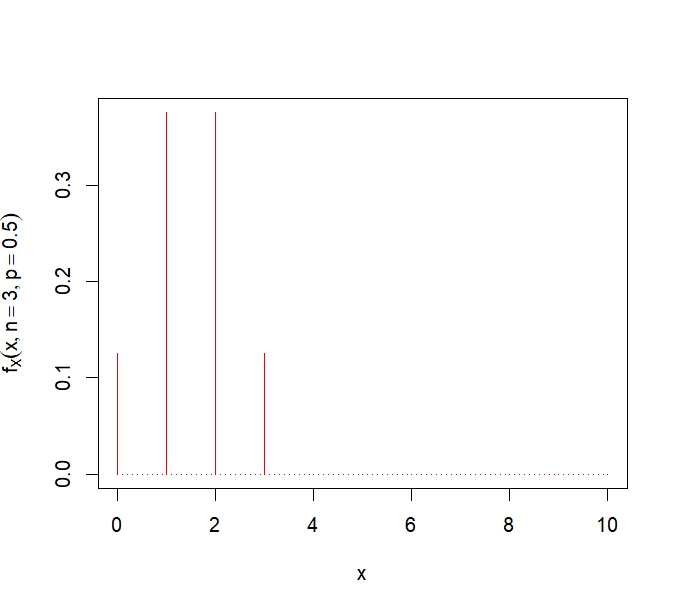
\includegraphics[scale=1]{Figuras/Binomial_n3.jpeg}
\caption{Función de masa de probabilidad binomial}
\end{figure}


\begin{example}
Experimento: Se lanza una moneda una vez, los resultados son águila y sol. La v.a  $X$ representa el número de lanzamientos requeridos hasta obtener del primer éxito (Geométrica).
\vspace{5mm}

La serie de ensayos son independientes teniendo cada ensayo dos posibles resultados: éxito o fracaso. Sea $p=P($ el ensayo termina en éxito$)$.

\vspace{5mm}
De acuerdo con lo anterior se tiene lo siguiente
\begin{eqnarray*}
f_{X}(x) &=&P(X=k) \\
&=&P(\text{ el primer éxito ocurre en el k-ésimo ensayo}) \\
&=&P(\text{en los primeros (k-1) ensayos se tienen fracasos})P(\text{k-ésimo ensayo se tiene éxito}) \\
&=&P(\text{(}k-1\text{) fracasos})P(\text{el k-ésimo es éxito}) \\
&=&(1-p)^{k-1}p
\end{eqnarray*}
Luego $f_{X}(x)=(1-p)^{k-1}p$,  $k=1,2,...$
\end{example}

\begin{remark}
Este ejemplo denota una variable aleatoria Geométrica.
\end{remark}

\begin{definition}[Propiedades de la pmf]
Cualquier función con dominio $\mathbb{R}$ y contradominio $[0,1]$ es una función de densidad discreta si para algún conjunto contable, $x_{1},x_{2},...,x_{n},...$ se tiene que:
\begin{enumerate}
\item $f(x)=0,$ si $x\neq x_{j}$, $j=1,2,3....$
\item $f(x)>0$, si $x=x_{j}$, $j=1,2,3,...$
\item $\sum f(x_{j})=1$
\end{enumerate}
\end{definition}

\vspace{5mm}
\textbf{pmf Bernoulli}: Un experimento Bernoulli tiene exactamente dos posibles resultados, éxito o fracaso. Una v.a Bernoulli $X$ tiene la función de masa de probabilidad 
\begin{equation*}
P(X=1)=p\text{ y }P(X=0)=1-p
\end{equation*}%
donde $p$ es la probabilidad de éxito.

La función de masa de probabilidad para una v.a Bernoulli, también se puede escribir de la siguiente forma
\begin{equation*}
f_{X}(x;p)=P(X=x)=p^{x}(1-p)^{1-x}I_{\{0,1\}}(x)
\end{equation*}

es decir, 
\begin{equation*}
f(x;p)=p^{x}q^{1-x}\text{, \ }x=0,1
\end{equation*}%
donde $0\leq p\leq 1$ y $q=1-p.$

\vspace{5mm}
\textbf{pmf Binomial:} Si $X$ registra el número de éxitos de $n$ ensayos Bernoulli independientes e idénticamente distribuidos (iid), con probabilidad de éxito $p.$ Entonces $X$ tiene función de masa de probabilidad Binomial($n,p$) dada por 
\begin{equation*}
f_{X}(x;p,n)=P(X=x)=\left( 
\begin{array}{c}
n \\ 
x
\end{array}
\right) p^{x}(1-p)^{n-x}
\end{equation*}%
donde $x=0,1,...,n.$

En otras palabras: 
\begin{equation*}
f(x;p,n)=\left( 
\begin{array}{c}
n \\ 
x
\end{array}%
\right) p^{x}q^{n-x}\text{, \ }x=0,1,2,...,n
\end{equation*}%
donde $0\leq p\leq 1$ y $q=1-p$, donde $p+q=1.$

\vspace{5mm}
\textbf{pmf Multinomial}: en un experimento dado con $n$ ensayos; para cada ensayo ocurren $k$ eventos mutuamente disjuntos $A_{1},...,A_{k}$ con probabilidad $P(A_{j})=p_{j}$, \ $j=1,...,k$.

Note que, si en un pmf binomial se tienen $n$ ensayos Bernoulli con dos posibles resultados y la probabilidad de éxito, $p$, es la misma en cada ensayo, en la pmf multinomial se tienen $n$ ensayos y en cada ensayo se tienen $k$ posibles resultados con probabilidades $P(A_{j})=p_{j}$,  $j=1,...,k$.

Dada $X_{j}$ la v.a que registra el número de veces que el evento $A_{j}$ ocurre en los $n$ ensayos idénticos e independientes del experimento. Entonces la función de masa de probabilidad está dada por
\begin{eqnarray*}
f(x_{1},x_{2},...,x_{k};p_{1},...,p_{k},n) &=&\left( 
\begin{array}{c}
n \\ 
x_{1},\text{ }x_{2},...,\text{ }x_{k}
\end{array}%
\right) p_{1}^{x_{1}}p_{2}^{x_{2}}\cdots p_{k}^{x_{k}} \\
&=&\frac{n!}{x_{1}!x_{2}!\cdots x_{k}!}p_{1}^{x_{1}}p_{2}^{x_{2}}\cdots
p_{k}^{x_{k}}
\end{eqnarray*}%
donde $\sum_{j=1}^{k}p_{k}=1$ y $\sum_{j=1}^{k}x_{j}=n$ con $0\leq x_{j}\leq
n$.

\vspace{5mm}
\textbf{pmf Uniforme}: 
\begin{equation*}
f(x;N)=\frac{1}{N}\text{, \ }x=1,2,...N
\end{equation*}

$N=1,2,...$
\vspace{5mm}
\textbf{pmf Poisson}
\begin{equation*}
f(x;\lambda )=\frac{e^{-\lambda }\lambda ^{x}}{x!}\text{, \ \ }x=0,1,2,...,
\end{equation*}%
donde $0\leq \lambda <\infty$.

\vspace{5mm}
\textbf{pmf Geométrica}: 
\begin{equation*}
f_{X}(x;p)=pq^{x-1}\text{ \ \ }x=1,2,..
\end{equation*}%
donde $0\leq p\leq 1$ y $q=1-p$


%%%%%%%%%%%%%%%%%%%%%%%%%%%%%%%%%%%%%%%%%%%%%
\subsection{Función de densidad de probabilidad}

\begin{definition}[pdf]
Si $X$ es una variable aleatoria continua, a su función $f_{X}(\cdot)$  se le llama función de densidad de probabilidad (\textbf{pdf}), y cumple con
\begin{equation*}
F_{X}(x)=\int_{-\infty }^{x}f_{X}(u)du
\end{equation*}
\end{definition}

\begin{definition}[Propiedades de la pdf]
Cualquier función $f_{X}(\cdot )$ con dominio $\mathbb{R}$ y contradominio $[0,\infty )$ es una función de densidad de probabilidad si y solo sí:
\begin{enumerate}
\item $f_{X}(x)\geq 0,$ $\forall x$
\item $\int_{-\infty }^{\infty }f_{X}(x)dx=1$
\end{enumerate}
\end{definition}

\textbf{pdf t}: William Sealy Gosset era un matemático y químico inglés que después de terminar sus estudios comenzó a trabajar en las destilerías Guinness, en lo que se refiere a control de calidad en el proceso de creación de la cerveza. Los tamaños pequeños de las muestras con los que habitualmente contaba fueron los responsables de sus estudios, y los que a la postre lo llevaron a desarrollar la distribución t. En $1908$, publico el artículo $\emph{The}$ $\emph{probable}$ $\emph{error}$ $\emph{of}$ $\emph{a}$ $\emph{mean}$ en la revista Biometrika con el seudónimo Student. La distribución $t$ de Student es una distribución de probabilidad que aparece cuando se quiere estimar la media de una población cuando el tamaño de la muestra utilizada para la estimación es pequeña y la varianza de la población es desconocida.


La distribución de probabilidad $t$ está dada por
\begin{equation*}
f_{X}(x;k)=\frac{\Gamma ((k+1)/2)}{\Gamma (k/2)}\frac{1}{\sqrt{k\pi }}\frac{1
}{\left( 1+\frac{x^{2}}{k}\right) ^{(k+1)/2}}\text{, }-\infty <x<\infty
\end{equation*}
donde $k>0.$

\textbf{pdf uniforme}: 
\begin{equation*}
f(x;a,b)=\frac{1}{b-a}\text{, \ }x\in \lbrack a,b]
\end{equation*}%
donde $-\infty <a<b<\infty$.

\textbf{pdf exponencial}:
\begin{equation*}
f(x;\lambda )=\lambda e^{-\lambda x}\text{ }x\in (0,\infty )
\end{equation*}%
donde $\lambda >0.$


\textbf{pdf normal:}
\begin{equation*}
f_{X}(x;\mu ,\sigma )=\frac{1}{\sqrt{2\pi \sigma ^{2}}}e^{-\frac{1}{2}\left( 
\frac{x-\mu }{\sigma }\right) ^{2}}
\end{equation*}
donde $-\infty <\mu <\infty $, \ $\sigma >0$ y $-\infty <x<\infty $


\textbf{pdf Cauchy:}
\begin{equation*}
f_{X}(x;\mu ,\sigma )=\frac{1}{\pi \beta \left[ 1+\left( \frac{x-\alpha }{%
\beta }\right) ^{2}\right] }
\end{equation*}
donde $-\infty <\alpha <\infty $, \ $\beta >0$ y $-\infty <x<\infty $


%%%%%%%‰%%%%%%%%%%%%%%%%%%%%%%%%%%%%%%%%
\subsection{Función de distribución acumulativa}

\begin{definition}[cdf]
La función de distribución acumulada (\textbf{cdf}) de una v.a $X$, es una función con dominio la recta real y contradominio el intervalo $[0,1]$,
\begin{equation*}
F_{X}:\mathbb{R}
\rightarrow \lbrack 0,1]
\end{equation*}
que satisface que 
\begin{eqnarray*}
F_{X}(x) &=&P(X\leq x) \\
&=&P(\{\omega \in \Omega :X(\omega )\leq x\})
\end{eqnarray*}
para todo $x\in \mathbb{R}$
\end{definition}

\vspace{5mm}
Una v.a $X$ continua tiene cdf, $F_{X},$ continua. Una variable aleatoria $X$ discreta tiene cdf, $F_{X},$ discreta, y es una función escalonada, "step".

\vspace{5mm}
\textbf{cdf v.a Discreta}: Dada $X$ una v.a discreta con $\mathcal{X}=\{x_{1},x_{2},...\}$ , la cdf $F_{X}(\cdot )$ puede ser obtenida de la pdf $f_{X}(\cdot )$ y viceversa; ya que 
\begin{equation*}
F_{X}(x)=\sum_{\{j\text{ }:\text{ }x_{j}\leq x\}}f_{X}(x_{j})
\end{equation*}
y 
\begin{equation*}
f_{X}(x_{j})=F_{X}(x_{j})-\lim_{0<h\rightarrow 0}F_{X}(x_{j}-h)
\end{equation*}

\textbf{cdf v.a Continua}: Dada $X$ una v.a continua, la cdf $F_{X}(\cdot )$ puede ser obtenida de la pdf $f_{X}(\cdot )$ y viceversa; ya que si $X$ es una v.a continua y $f_{X}(x)$ está dada, entonces $F_{X}(x)$ es obtenida a partir de integrar $f_{X}(x)$, es decir,
\begin{equation*}
F_{X}(x)=P(X\leq x)=\int_{-\infty }^{x}f_{X}(u)du
\end{equation*}


\section{Distribuciones de probabilidad de variables aleatorias discretas}

%%%%%%%%%%%%%%%%%%%%%%%%%%%%%%%%%%%%%%%%%%%%%%%
\subsection{Uniforme discreta}

\begin{definition}
La distribución uniforme discreta está dada por 
\begin{equation*}
f_{X}(x)=f_{X}(x;N)=P(X=x)=\left\{ 
\begin{array}{l}
1/N\text{, si }x\in \mathcal{X} \\ 
0,\text{ si }x\notin \mathcal{X}
\end{array}
\right.
\end{equation*}
es decir 
\begin{equation*}
f_{X}(x;N)=\frac{1}{N}I_{\{1,2,...,N\}}(x)
\end{equation*}
\end{definition}


\begin{i}

\begin{theorem}
Si $X$ tiene distribución uniforma discreta, entonces
\begin{equation*}
E(X)=\frac{N+1}{2}
\end{equation*}
\begin{equation*}
Var(X)=\frac{N^{2}-1}{12}
\end{equation*}
y 
\begin{equation*}
m_{X}(t)=\sum\limits_{j=1}^{N}e^{tj}\frac{1}{N}\text{ //}j=x
\end{equation*}
\end{theorem}

Demostración: Dado que

\begin{equation*}
E(X)=\sum x_{j}f_{X}(x_{j})
\end{equation*}%
entonces%
\begin{eqnarray*}
E(X) &=&\sum_{j=1}^{N}j\frac{1}{N}\text{ \ \ //}x=j \\
&=&\frac{1}{N}\sum_{j=1}^{N}j\text{ \ \ //inducción} \\
&=&\frac{1}{N}\frac{N(N+1)}{2}=\frac{N+1}{2}
\end{eqnarray*}

Luego 
\begin{equation*}
E(X)=\frac{N+1}{2}
\end{equation*}

Por otra parte, note que 
\begin{eqnarray*}
E(X^{2}) &=&\sum_{j=1}^{N}j^{2}\frac{1}{N}\text{ \ //}x=j \\
&=&\frac{1}{N}\sum_{j=1}^{N}j^{2}\text{ // inducción} \\
&=&\frac{1}{N}\frac{N(N+1)(2N+1)}{6} \\
&=&\frac{(N+1)(2N+1)}{6}
\end{eqnarray*}
Como 
\begin{equation*}
V(X)=E(X^{2})-[E(X)]^{2}
\end{equation*}
entonces
\begin{eqnarray*}
V(X) &=&\frac{(N+1)(2N+1)}{6}-\frac{\left( N+1\right) ^{2}}{4} \\
&=&(N+1)\left( \frac{2N+1}{6}-\frac{\left( N+1\right) }{4}\right) \\
&=&(N+1)\left( \frac{4N+2-3N-3}{12}\right) \\
&=&(N+1)\left( \frac{N-1}{12}\right) \\
&=&\frac{N^{2}-1}{12}
\end{eqnarray*}
luego
\begin{equation*}
V(X)=\frac{N^{2}-1}{12}
\end{equation*}

Finalmente
\begin{eqnarray*}
m_{X}(t) &=&E(e^{tX}) \\
&=&\sum\limits_{j=1}^{N}e^{tj}\frac{1}{N}\text{ //}x=j \\
&=&\frac{1}{N}\sum\limits_{j=1}^{N}e^{tj}
\end{eqnarray*}

%%%%%%%%%%%%%%%%%%%%%%%%%%%%%%%%%%%%%
\subsection{Bernoulli}

\begin{definition}
Una v.a $X$ tiene distribución Bernoulli si la pmf de $X$ está dada por 
\begin{equation*}
f_{X}(x)=f_{X}(x;p)=P(X=x)=\left\{ 
\begin{array}{l}
p^{x}(1-p)^{1-x}\text{, si }x\in \mathcal{X}=\{0,1\} \\ 
0\text{ si }x\notin \mathcal{X}
\end{array}
\right.
\end{equation*}
es decir
\begin{equation*}
f_{X}(x,p)=p^{x}(1-p)^{1-x}I_{\{0,1\}}(x)
\end{equation*}%
donde $0\leq p\leq 1.$ Si $q=1-p$, entonces
\begin{equation*}
f_{X}(x)=p^{x}q^{1-x}I_{\{0,1\}}(x)
\end{equation*}
\end{definition}

\begin{figure}[h!]
\centering
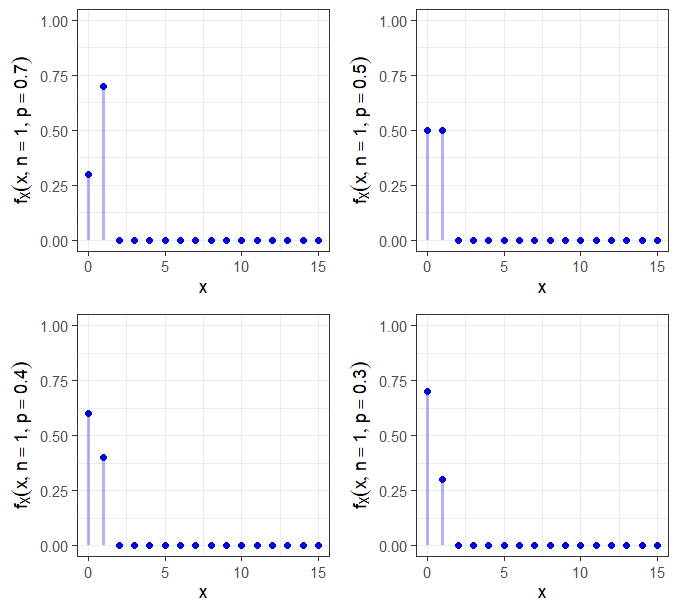
\includegraphics[scale=1]{Figuras/Bernoulli.jpeg}
\caption{Función de masa de probabilidad Bernoulli}
\end{figure}

\begin{theorem}
Si $X$ tiene distribución Bernoulli, entonces 
\begin{eqnarray*}
E(X) &=&p \\
V(X) &=&pq \\
m_{X}(t) &=&pe^{t}+q
\end{eqnarray*}
\end{theorem}

Demostración:
\begin{eqnarray*}
E(X) &=&\sum_{x\in \mathcal{X}}xf_{X}(x) \\
&=&\sum_{x\in \mathcal{X}}xp^{x}(1-p)^{1-x} \\
&=&0p^{0}(1-p)^{1-0}+1p^{1}(1-p)^{1-1} \\
&=&p
\end{eqnarray*}
Por lo tanto
\begin{equation*}
E(X)=p
\end{equation*}

Por otra parte 
\begin{eqnarray*}
E(X^{2}) &=&\sum_{x}x^{2}f_{X}(x) \\
&=&\sum_{x\in \mathcal{X}}x^{2}p^{x}(1-p)^{1-x} \\
&=&0^{2}p^{0}(1-p)^{1-0}+1^{2}p^{1}(1-p)^{1-1} \\
&=&p
\end{eqnarray*}
Entonces
\begin{eqnarray*}
V(X) &=&E(X^{2})-[E(X)]^{2} \\
&=&p-p^{2} \\
&=&p(1-p)\text{ //}q=1-p \\
&=&pq
\end{eqnarray*}
Por lo tanto
\begin{equation*}
V(X)=pq
\end{equation*}

Finalmente note que 
\begin{eqnarray*}
m_{X}(t) &=&E(e^{tX}) \\
&=&\sum_{x\in \mathcal{X}}e^{tx}f(x) \\
&=&\sum_{x=0}^{1}e^{tx}p^{x}(1-p)^{1-x} \\
&=&e^{t0}p^{0}(1-p)^{1-0}+e^{t}p^{1}(1-p)^{1-1} \\
&=&(1-p)+e^{t}p
\end{eqnarray*}
Por lo tanto
\begin{equation*}
m_{X}(t)=e^{t}p+q
\end{equation*}

%%%%%%%%%%%%%%%%%%%%%%%%%%%%%%%%%%%%%%
\subsection{Binomial}

\begin{definition}
Una v.a $X$ tiene distribución Binomial si la pmf de $X$ está dada por 
\begin{equation*}
f_{X}(x)=f_{X}(x;n,p)=P(X=x)=\left\{ 
\begin{array}{l}
\binom{n}{x}p^{x}q^{1-x}\text{, si }x\in \mathcal{X}=\{0,1,...,n\} \\ 
0,\text{ si }x\notin \mathcal{X}%
\end{array}%
\right.
\end{equation*}%
Es decir;
\begin{equation*}
f_{X}(x;n,p)=\binom{n}{x}p^{x}q^{1-x}I_{\{0,1,...,n\}}(x)
\end{equation*}%
donde $0\leq p\leq 1$, $q=1-p$.
\end{definition}

\begin{figure}[h!]
\centering
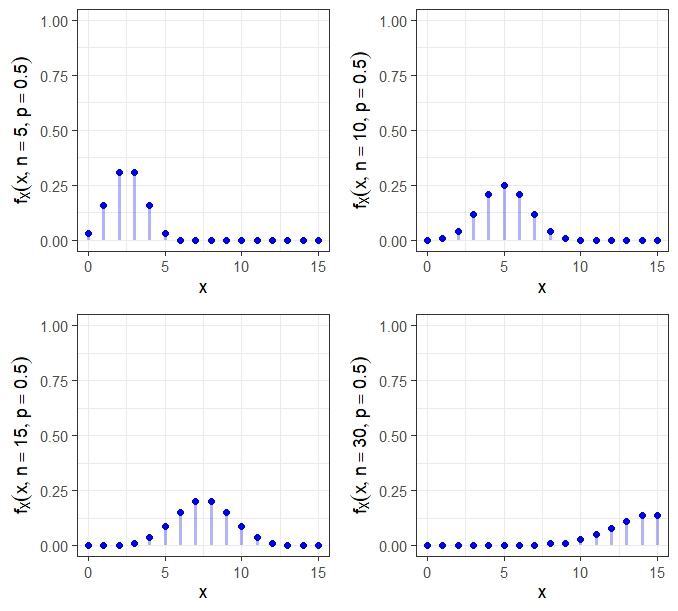
\includegraphics[scale=1]{Figuras/Binomial.jpeg}
\caption{Función de masa de probabilidad Binomial}
\end{figure}

\begin{theorem}
Si $X$ tiene distribución binomial, entonces
\begin{eqnarray*}
E(X) &=&np \\
V(X) &=&npq \\
m_{X}(t) &=&\left( q+pe^{t}\right) ^{n}
\end{eqnarray*}
\end{theorem}

Demostración: Se deduce primero la fgm 
\begin{eqnarray*}
m_{X}(t) &=&E(e^{tX}) \\
&=&\sum_{x}e^{tx}\binom{n}{x}p^{x}q^{1-x} \\
&=&\sum_{x=0}^{n}\binom{n}{x}\left( pe^{t}\right) ^{x}q^{1-x}\text{ //}
\sum_{j=0}^{n}\binom{n}{j}a^{j}b^{n-j}=(a+b)^{n} \\
&=&(pe^{t}+q)^{n}
\end{eqnarray*}
es decir, 
\begin{equation*}
m_{X}(t)=(pe^{t}+q)^{n}
\end{equation*}

Dado que 
\begin{equation*}
E(X)=\frac{d}{dt}m_{X}(t)
\end{equation*}

Entonces
\begin{equation*}
\frac{d}{dt}m_{X}(t)=n(pe^{t}+q)^{n-1}pe^{t}
\end{equation*}%
luego%
\begin{eqnarray*}
\left. \frac{d}{dt}m_{X}(t)\right\vert _{t=0} &=&n(pe^{0}+q)^{n-1}pe^{0} \\
&=&np
\end{eqnarray*}%
entonces
\begin{equation*}
E(X)=np
\end{equation*}

Por otra parte
\begin{equation*}
E(X^{2})=\frac{d^{2}}{dt^{2}}m_{X}(t)
\end{equation*}
Entonces
\begin{equation*}
\frac{d^{2}}{dt^{2}}
m_{X}(t)=n(n-1)(pe^{t}+q)^{n-2}p^{2}e^{2t}+pe^{t}n(pe^{t}+q)^{n-1}
\end{equation*}
luego
\begin{eqnarray*}
\left. \frac{d^{2}}{dt^{2}}m_{X}(t)\right\vert _{t=0}
&=&n(n-1)(pe^{0}+q)^{n-2}p^{2}e^{2(0)}+pe^{0}n(pe^{0}+q)^{n-1} \\
&=&n(n-1)(p+1-p)^{n-2}p^{2}+pn(p+1-p)^{n-1} \\
&=&n(n-1)p^{2}+pn
\end{eqnarray*}
entonces
\begin{equation*}
E(X^{2})=n(n-1)p^{2}+pn
\end{equation*}
Finalmente 
\begin{eqnarray*}
V(X) &=&E(X^{2})-[E(X)]^{2} \\
&=&n^{2}p^{2}-np^{2}+pn-n^{2}p^{2} \\
&=&pn-np^{2} \\
&=&n(p-p^{2}) \\
&=&n(p(1-p)) \\
&=&npq
\end{eqnarray*}
luego%
\begin{equation*}
V(X)=npq
\end{equation*}
%%%%%%%%%%%%%%%%%%%%%%%%%%%%%%%%%%%%%%%%%
\subsubsection{Resolución de problemas}

Para $X$, una variable aleatoria Binomial con $n=5$ y $p=0.5$, calcular su media y varianza.

\begin{figure}[h!]
\centering
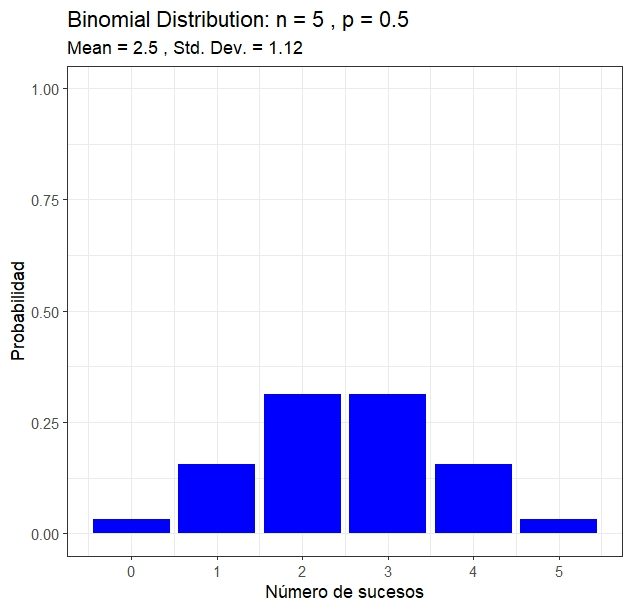
\includegraphics[scale=0.8]{Figuras/Binomial_n5.jpeg}
\caption{Función de masa de probabilidad Binomial}
\end{figure}

Para $X$, una variable aleatoria Binomial con $n=10$ y $p=0.5$, calcular su media y varianza. 

\begin{figure}[h!]
\centering
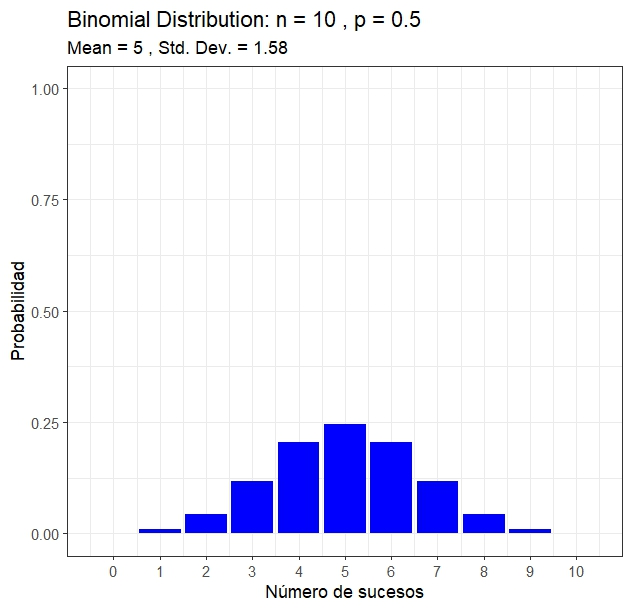
\includegraphics[scale=0.8]{Figuras/Binomial_n10.jpeg}
\caption{Función de masa de probabilidad Binomial}
\end{figure}


%%%%%%%%%%%%%%%%%%%%%%%%%%%%%%%%%%%%%%%%%
\subsubsection{Práctica con R}
%%%%%%%%%%%%%%%%%%%%%%%%%%%%%%%%%%%%%%%%%
% Agragar gráficos dinámicos


%%%%%%%%%%%%%%%%%%%%%%%%%%%%%%%%%%%%%%%%%%%%%%%%%%
\subsection{Hipergeométrica}

\begin{definition}
Una v.a $X$ tiene distribución hipergeométrica si su pmf está dada por 
\begin{equation*}
f_{X}(x,M,n,K)=\frac{\binom{K}{x}\binom{M-K}{n-x}}{\binom{M}{n}}\text{, }%
x=0,1,..,n
\end{equation*}
donde
$M=1,2,...$
$K=0,1,...,M$
$n=1,2,...,M$
\end{definition}

Note que 
\begin{equation*}
f_{X}(x,M,n,K)=\frac{\binom{K}{x}\binom{M-K}{n-x}}{\binom{M}{n}}
I_{\{0,1,...,n\}}(x).
\end{equation*}

\begin{figure}[h!]
\centering
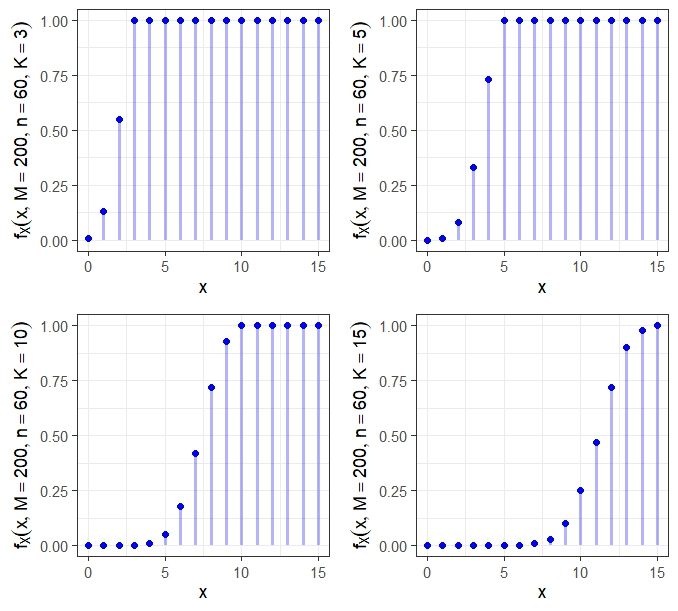
\includegraphics[scale=1]{Figuras/Hipergeometrica.jpeg}
\caption{Función de masa de probabilidad Hipergeométrica}
\end{figure}

\begin{theorem}
Si $X$ tiene distribución hipergeométrica, entonces
\begin{eqnarray*}
E(X) &=&n\frac{K}{M} \\
V(X) &=&n\cdot \frac{K}{M}\cdot \frac{M-K}{M}\cdot \frac{M-n}{M-1}
\end{eqnarray*}
\end{theorem}

Demostración
\begin{eqnarray*}
E(X) &=&\sum_{x}xf_{X}(x) \\
&=&\sum_{x=0}^{n}x\frac{\binom{K}{x}\binom{M-K}{n-x}}{\binom{M}{n}} \\
&=&\sum_{x=1}^{n}x\frac{\binom{K}{x}\binom{M-K}{n-x}}{\binom{M}{n}}
\end{eqnarray*}

Usando la función indicadora, note que 
\begin{equation*}
x\binom{K}{x}=x\frac{K!}{x!(K-x)!}=\frac{K!}{\left( x-1\right) !(K-x)!}=%
\frac{K(K-1)!}{\left( x-1\right) !(K-x)!}=K\binom{K-1}{x-1}
\end{equation*}

\begin{equation*}
\binom{M}{n}=\frac{M!}{n!(M-n)!}=\frac{M(M-1)!}{n(n-1)!(M-n)!}=\frac{M}{n}
\binom{M-1}{n-1}
\end{equation*}
Entonces
\begin{eqnarray*}
\sum_{x=1}^{n}x\frac{\binom{K}{x}\binom{M-K}{n-x}}{\binom{M}{n}}
&=&\sum_{x=1}^{n}\frac{K\binom{K-1}{x-1}\binom{M-K}{n-x}}{\frac{M}{n}\binom{
M-1}{n-1}} \\
&=&n\frac{K}{M}\sum_{x=1}^{n}\frac{\binom{K-1}{x-1}\binom{M-K}{n-x}}{\binom{
M-1}{n-1}}
\end{eqnarray*}

Sea $y=x-1$ entonces $x=y+1$, luego 
\begin{eqnarray*}
E(X) &=&n\frac{K}{M}\sum_{y=0}^{n-1}\frac{\binom{K-1}{y}\binom{M-1-K+1}{n-1-y%
}}{\binom{M-1}{n-1}}//pmf \\
&=&n\frac{K}{M}
\end{eqnarray*}

Por otra parte, el segundo momento factorial de $X$ está dado por%
\begin{eqnarray*}
E[X(X-1)] &=&\sum_{x=0}^{n}x(x-1)\frac{\binom{K}{x}\binom{M-K}{n-x}}{\binom{M%
}{n}} \\
&=&\sum_{x=2}^{n}x(x-1)\frac{\binom{K}{x}\binom{M-K}{n-x}}{\binom{M}{n}}
\end{eqnarray*}

Note que
\begin{eqnarray*}
x(x-1)\binom{K}{x} &=&x(x-1)\frac{K!}{x!(K-x)!} \\
&=&\frac{K(K-1)(K-2)!}{(x-2)!(K-x)!} \\
&=&K(K-1)\binom{K-2}{x-2}
\end{eqnarray*}
y 
\begin{equation*}
\binom{M}{n}=\frac{M!}{n!(M-n)!}=\frac{M(M-1)(M-2)!}{n(n-1)(n-2)!(M-n)!}=
\frac{M}{n}\cdot \frac{\left( M-1\right) }{\left( n-1\right) }\binom{M-2}{n-2
}
\end{equation*}
Sustituyendo
\begin{eqnarray*}
E[X(X-1)] &=&\sum_{x=2}^{n}\frac{K(K-1)\binom{K-2}{x-2}\binom{M-K}{n-x}}{%
\frac{M}{n}\frac{\left( M-1\right) }{\left( n-1\right) }\binom{M-2}{n-2}} \\
&=&n(n-1)\frac{K(K-1)}{M\left( M-1\right) }\sum_{x=2}^{n}\frac{\binom{K-2}{
x-2}\binom{M-K}{n-x}}{\binom{M-2}{n-2}}
\end{eqnarray*}

Sea $y=x-2$, entonces $x=y+2$, luego
\begin{equation*}
\sum_{y=0}^{n-2}\frac{\binom{K-2}{y}\binom{M-2-K+2}{n-2-y}}{\binom{M-2}{n-2}}
=1\text{ //pmf}
\end{equation*}
entonces
\begin{equation*}
E[X(X-1)]=n(n-1)\frac{K(K-1)}{M\left( M-1\right) }
\end{equation*}

Como
\begin{eqnarray*}
E[X(X-1)] &=&E[X^{2}-X] \\
&=&E(X^{2})-E(X)
\end{eqnarray*}
Entonces, despejando
\begin{equation*}
E(X^{2})=E[X(X-1)]+E(X)
\end{equation*}

Luego

\begin{eqnarray*}
V(X) &=&E(X^{2})-[E(X)]^{2}\text{ \ //Def.} \\
&=&E[X(X-1)]+E(X)-[E(X)]^{2} \\
&=&n(n-1)\frac{K(K-1)}{M\left( M-1\right) }+\frac{nK}{M}-\frac{n^{2}K^{2}}{
M^{2}} \\
&=&n\frac{K}{M}\left[ (n-1)\frac{(K-1)}{\left( M-1\right) }+1-\frac{nK}{M}
\right] \\
&=&n\frac{K}{M}\left[ (n-1)\frac{(K-1)}{\left( M-1\right) }+\frac{M-nK}{M}
\right] \\
&=&n\frac{K}{M}\left[ \frac{(n-1)(KM-M)+M^{2}-M-nKM+nK}{M\left( M-1\right) }%
\right] \\
&=&n\frac{K}{M}\frac{1}{M(M-1)}\left[ nKM-KM-nM+M+M^{2}-M-nKM+nK\right] \\
&=&n\frac{K}{M}\frac{1}{M(M-1)}\left( M^{2}-KM-nM+nK\right) \\
&=&n\frac{K}{M}\frac{1}{M(M-1)}(M-K)(M-n)
\end{eqnarray*}%
luego%
\begin{equation*}
V(X)=n\frac{K}{M}\cdot \frac{M-K}{M}\cdot \frac{M-n}{M-1}
\end{equation*}


%%%%%%%%%%%%%%%%%%%%%%%%%%%%%%%%%%%%%%%
\subsection{Poisson}

\begin{definition}
Una v.a $X$ tiene distribución Poisson, si 
\begin{equation*}
f(x;\lambda )=\frac{e^{-\lambda }\lambda ^{x}}{x!}I_{\{0,1,...\}}(x)
\end{equation*}%
con $\lambda >0.$
\end{definition}

\begin{figure}[h!]
\centering
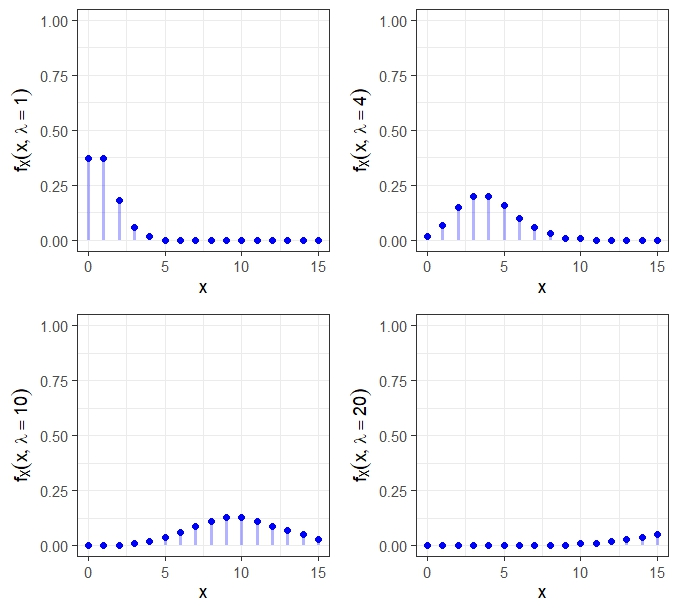
\includegraphics[scale=1]{Figuras/Poisson.jpeg}
\caption{Función de masa de probabilidad Poisson.}
\end{figure}

\begin{theorem}
Si la v.a $X$ tiene distribución Poisson, entonces
\begin{eqnarray*}
E(X) &=&\lambda \\
V(X) &=&\lambda \\
m_{X}(t) &=&e^{\lambda (e^{t}-1)}
\end{eqnarray*}
\end{theorem}

Demostración:
\begin{eqnarray*}
E(X) &=&\sum_{x}xf(x) \\
&=&\sum_{x=0}^{\infty }x\frac{e^{-\lambda }\lambda ^{x}}{x!} \\
&=&e^{-\lambda }\sum_{x=0}^{\infty }x\frac{\lambda ^{x}}{x!} \\
&=&\lambda e^{-\lambda }\sum_{x=1}^{\infty }\frac{\lambda ^{x-1}}{(x-1)!}
\end{eqnarray*}
sea $y=x-1$, entonces
\begin{eqnarray*}
E(X) &=&\lambda e^{-\lambda }\sum_{y=0}^{\infty }\frac{\lambda ^{y}}{y!}%
\text{ \ \ //}\sum_{j=0}^{\infty }\frac{x^{j}}{j!}=e^{x} \\
&=&\lambda e^{-\lambda }e^{\lambda } \\
&=&\lambda
\end{eqnarray*}
Por otra parte
\begin{eqnarray*}
E(X(X-1)) &=&\sum_{x=0}^{\infty }x(x-1)\frac{e^{-\lambda }\lambda ^{x}}{x!}
\\
&=&e^{-\lambda }\sum_{x=2}^{\infty }\frac{\lambda ^{x}}{(x-2)!} \\
&=&\lambda ^{2}e^{-\lambda }\sum_{x=2}^{\infty }\frac{\lambda ^{x-2}}{(x-2)!}
\end{eqnarray*}
sea $y=x-2$

entonces
\begin{eqnarray*}
E(X(X-1)) &=&\lambda ^{2}e^{-\lambda }\sum_{y=0}^{\infty }\frac{\lambda ^{y}%
}{y!} \\
&=&\lambda ^{2}e^{-\lambda }e^{\lambda } \\
&=&\lambda ^{2}
\end{eqnarray*}
Como 
\begin{eqnarray*}
V(X) &=&E(X(X-1))+E(X)-[E(X)]^{2} \\
&=&\lambda ^{2}+\lambda -\lambda ^{2} \\
&=&\lambda
\end{eqnarray*}
Luego 
\begin{equation*}
V(X)=\lambda
\end{equation*}

Por otra parte; 
\begin{eqnarray*}
m_{X}(t) &=&E(e^{tX}) \\
&=&\sum_{x=0}^{\infty }e^{tx}\frac{e^{-\lambda }\lambda ^{x}}{x!} \\
&=&e^{-\lambda }\sum_{x=0}^{\infty }\frac{\left( e^{t}\lambda \right) ^{x}}{
x!} \\
&=&e^{-\lambda }e^{\lambda e^{t}} \\
&=&e^{\lambda e^{t}}e^{-\lambda } \\
&=&e^{\lambda \left( e^{t}-1\right) }
\end{eqnarray*}

Por lo tanto
\begin{equation*}
m_{X}(t)=e^{\lambda \left( e^{t}-1\right) }
\end{equation*}


%%%%%%%%%%%%%%%%%%%%%%%%%%%%%%%%%%%%%%%%%%%
\subsection{Binomial negativa}

\begin{definition}
Una v.a $X$ con distribución binomial negativa, está dada por 
\begin{equation*}
f(x;r,p)=\binom{r+x-1}{x}p^{r}q^{x}=\binom{-r}{x}p^{r}(-q)^{x}\text{, \ \ \
\ }x=0,1,2,...
\end{equation*}
donde $0<p\leq 1,$ $q=1-p$ $\ $y $r=1,2,3,...$ 
\end{definition}

\begin{figure}[h!]
\centering
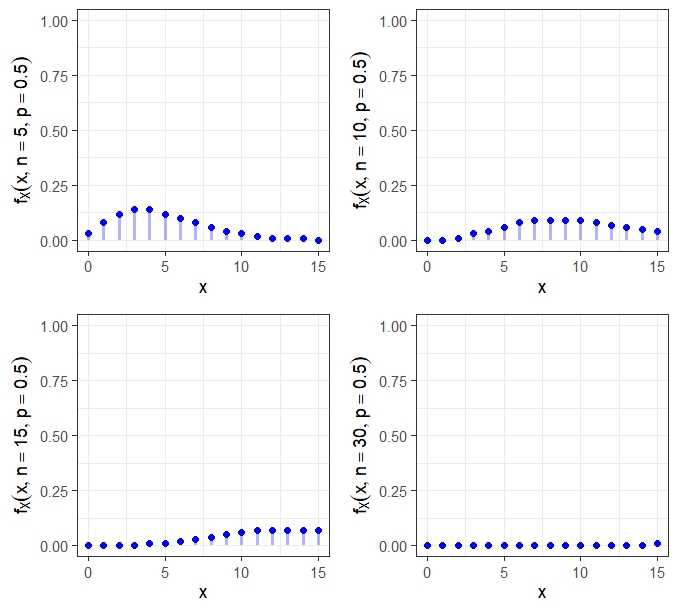
\includegraphics[scale=1]{Figuras/Binomial_negativa.jpeg}
\caption{Función de masa de probabilidad Binomial negatica}
\end{figure}


\begin{theorem}
Si $X$ tiene distribución binomial negativa, entonces
\begin{eqnarray*}
E(X) &=&\frac{rq}{p} \\
V(X) &=&\frac{rq}{p^{2}} \\
m_{X}(t) &=&\left( \frac{p}{1-qe^{t}}\right) ^{r}
\end{eqnarray*}
\end{theorem}

Demostración: 
\begin{eqnarray*}
m_{X}(t) &=&E(e^{tX}) \\
&=&\sum_{x=0}^{\infty }e^{tx}\binom{-r}{x}p^{r}(-q)^{x} \\
&=&\sum_{x=0}^{\infty }\binom{-r}{x}p^{r}(-qe^{t})^{x} \\
&=&p^{r}\sum_{x=0}^{\infty }\binom{-r}{x}(-qe^{t})^{x}\text{ //}
\sum_{j=0}^{\infty }\binom{t}{j}(-x)^{j}=(1-x)^{t}\text{, }-1<x<1 \\
&=&p^{r}\left( 1-qe^{t}\right) ^{-r}\text{, \ \ }0<q<1,\text{ }0<p\leq 1
\end{eqnarray*}

i.e,
\begin{equation*}
m_{X}(t)=\left( \frac{p}{1-qe^{t}}\right) ^{r}
\end{equation*}

Cálculo de la esperanza:
\begin{eqnarray*}
\frac{d}{dt}m_{x}(t) &=&r\left( \frac{p}{1-qe^{t}}\right) ^{r-1}\left[ \frac{%
0-(-qe^{-t})p}{\left( 1-qe^{t}\right) ^{2}}\right] \\
&=&r\frac{p^{r-1}}{\left( 1-qe^{t}\right) ^{r-1}}\left( \frac{qpe^{t}}{%
\left( 1-qe^{t}\right) ^{2}}\right) \\
&=&\frac{rp^{r}qe^{t}}{\left( 1-qe^{t}\right) ^{r+1}}
\end{eqnarray*}
luego
\begin{equation*}
\left. \frac{d}{dt}m_{X}(t)\right\vert _{t=0}=\frac{rp^{r}qe^{0}}{\left(
1-qe^{0}\right) ^{r+1}}=\frac{rp^{r}q}{\left( 1-(1-p)\right) ^{r+1}}=\frac{
rp^{r}q}{p^{r+1}}=\frac{rq}{p}
\end{equation*}
Por lo tanto
\begin{equation*}
E(X)=\frac{rq}{p}
\end{equation*}

Por otra parte
\begin{equation*}
\left. \frac{d^{2}}{dt^{2}}m_{X}(t)\right\vert _{t=0}=\frac{r(q+q^{2}r)}{
p^{2}}=E(X^{2})
\end{equation*}
Luego 
\begin{eqnarray*}
V(X) &=&E(X^{2})-\left[ E(X)\right] ^{2} \\
&=&\frac{rq+q^{2}r^{2}}{p^{2}}-\frac{r^{2}q^{2}}{p^{2}} \\
&=&\frac{rq}{p^{2}}
\end{eqnarray*}
Por lo tanto
\begin{eqnarray*}
V(X)=\frac{rq}{p^{2}}
\end{eqnarray*}



%%%%%%%%%%%%%%%%%%%%%%%%%%%%%%%%%%%%%%%%%
\subsection{Geométrica}


Consideremos una serie de ensayos independientes donde cada ensayo tiene dos posibles resultados éxito o fracaso, y sea $p=P($ensayo es éxito$)$. Definiendo a $X$ como la v.a en el cual el primer éxito ocurre; entonces la pmf de $X$ está dada por
\begin{equation*}
f(x;p)=p(1-p)^{x}
\end{equation*}%
$x=0,1,2,3,...$

\begin{definition}
Una v.a $X$ tiene distribución geométrica, si la densidad de $X$ está dada por
\begin{equation*}
f(x;p)=p(1-p)^{x}I_{\{0,1,2,...\}}(x)
\end{equation*}%
donde $0<p\leq 1.$
\end{definition}

\begin{figure}[h!]
\centering
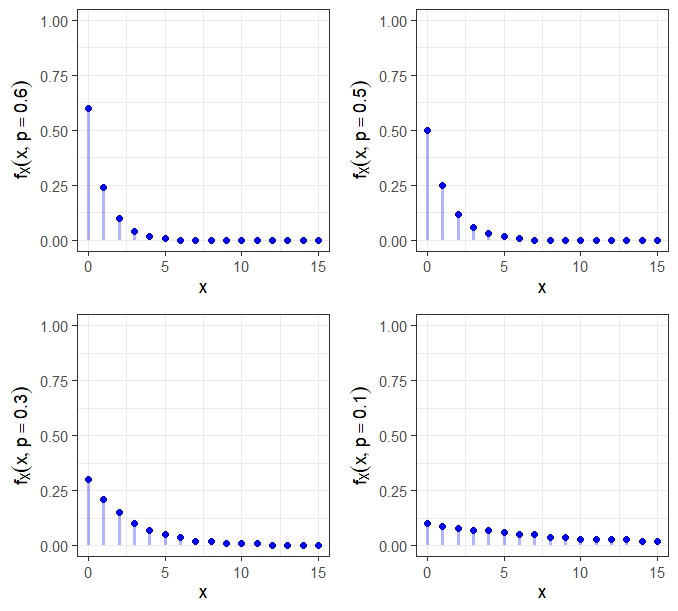
\includegraphics[scale=1]{Figuras/Geometrica.jpeg}
\caption{Función de masa de probabilidad Geométrica}
\end{figure}

\begin{theorem}
Si $X$ es una v.a con distribución geométrica dada por
\begin{equation*}
f(x;p)=p(1-p)^{x}I_{\{0,1,2,...\}}(x)
\end{equation*}%
\bigskip entonces%
\begin{eqnarray*}
E(X) &=&\frac{q}{p} \\
V(X) &=&\frac{q}{p^{2}} \\
m_{X}(t) &=&\frac{p}{1-qe^{t}}
\end{eqnarray*}
\end{theorem}

\textbf{Demostración}: Del Teorema de la Binomial negativa, se tiene el
resultado, para $r=1$.

\textbf{Observación}:
\begin{itemize}
\item La Binomial negativa es una generalización de la distribución geométrica, cuando se repiten los ensayos independientes, con probabilidad $p$, hasta obtener un número total de $r$ éxitos (pag. $95$, Casella, $1999$).

\item Existe al menos otra parametrización para la Binomial negativa.
\end{itemize}


\begin{definition}
La v.a $X$ tiene distribución Binomial negativa si su pmf está dada por 
\begin{equation*}
f(x,r,p)=\binom{x-1}{r-1}p^{r}(1-p)^{x-r}\text{, \ \ }x=r,r+1,...
\end{equation*}
\end{definition}

Note que $x-1$ son los primeros lanzamientos y $r-1$ son éxitos.
\textbf{Resultado:} Para una v.a $X$ con distribución Binomial negativa
dada por 
\begin{equation*}
f(x;r,p)=\binom{x-1}{r-1}p^{r}(1-p)^{x-r}\text{, \ \ }x=r,r+1,...
\end{equation*}%
se tiene que

\begin{eqnarray*}
E(X) &=&\frac{r}{p} \\
V(X) &=&\frac{rq}{p^{2}} \\
m(t) &=&\left( \frac{pe^{t}}{1-qe^{t}}\right) ^{r}
\end{eqnarray*}


\textbf{Tarea}: Demostrar el resultado anterior.

Note que para $r=1$ en la parametrización anterior, es decir,

\begin{equation*}
f(x;r,p)=\binom{x-1}{r-1}p^{r}(1-p)^{x-r}\text{, \ \ }x=r,r+1,...
\end{equation*}
se tiene que\ 
\begin{eqnarray*}
f(x;p) &=&\binom{x-1}{0}p(1-p)^{x-1} \\
&=&p(1-p)^{x-1}
\end{eqnarray*}
donde $x=1,2,...$

Es decir,
\begin{equation*}
f(x;p)=p(1-p)^{x-1}I_{\{1,2,3,..\}}(x)
\end{equation*}
es la parametrización de una variable aleatoria con distribución geométrica (Casella, $1999$).


\textbf{Resultado}: Si $X$ tiene distribución geométrica dada por
\begin{equation*}
f(x,r,p)=p(1-p)^{x-1}\text{, \ \ \ }x=1,2,..
\end{equation*}%
donde
\begin{eqnarray*}
E(X) &=&\frac{1}{p} \\
V(X) &=&\frac{q}{p^{2}} \\
m_{X}(t) &=&\frac{pe^{t}}{1-qe^{t}}
\end{eqnarray*}

\textbf{Tarea}: Demostrar el resultado anterior.


%%%%%%%%%%%%%%%%%%%%%%%%%%%%%%%%%%%%%%%%%%%%%%
\subsection{Logarítmica}

\begin{definition}
Una v.a $X$ con distribución logarítmica, está dada  por 
\begin{equation*}
f(x;p)=\frac{q^{x}}{-x\log _{e}(p)}I_{\{1,2,...\}}(x)
\end{equation*}%
donde $0<p<1$ y $q=1-p.$
\end{definition}

\begin{theorem}
 Si $X$ tiene distribución logarítmica, entonces
\begin{eqnarray*}
E(X) &=&\frac{q}{-p\log _{e}(p)} \\
&& \\
V(X) &=&\frac{q(q+\log _{e}(p))}{-(p\log _{e}(p))^{2}} \\
&& \\
m_{X}(t) &=&\frac{\log _{e}(1-qe^{t})}{\log _{e}(1-q)}
\end{eqnarray*}
\end{theorem}


\textbf{Tarea}: Deducir la $E(X)$ y la $V(X)$ a partir de la $m_{X}(t)$.


%%%%%%%%%%%%%%%%%%%%%%%%%%%%%%%%%%%%%%%%%%%%%%%%%%%%%%%%%%%%%%
\section{Distribuciones de probabilidad para v.a continuas}


%%%%%%%%%%%%%%%%%%%%%%%%%%%%%%%%%%%%%%%%%%%%%
\subsection{Uniforme continua}

\begin{definition}
Una v.a $X$ tiene distribución Uniforme en el intervalo $[a,b]$ si su pdf está dada por 
\begin{equation*}
f(x;a,b)=\frac{1}{b-a}I_{[a,b]}(x)
\end{equation*}%
donde $-\infty <a<b<\infty$.
\end{definition}

Note que:
\begin{itemize}
\item $b>a$

\item Cuando $X$ tiene distribución uniforme entonces se dice que $X\sim
U(a,b)$.
\end{itemize}


\begin{theorem}
 Si $X$ tiene distribución $U(a,b)$, entonces
\begin{eqnarray*}
E(X) &=&\frac{a+b}{2} \\
&& \\
V(X) &=&\frac{(b-a)^{2}}{12} \\
&& \\
m_{X}(t) &=&\frac{e^{bt}-e^{at}}{(b-a)t}
\end{eqnarray*}
\end{theorem} 

Demostración: 
\begin{eqnarray*}
E(X) &=&\int_{a}^{b}x\frac{1}{b-a}dx \\
&=&\frac{1}{b-a}\int_{a}^{b}xdx \\
&=&\frac{1}{b-a}\left. \frac{x^{2}}{2}\right\vert _{x=a}^{x=b} \\
&=&\frac{b^{2}-a^{2}}{2(b-a)} \\
&=&\frac{\left( b-a\right) \left( a+b\right) }{2(b-a)} \\
&=&\frac{a+b}{2}
\end{eqnarray*}

Por otra parte, 
\begin{eqnarray*}
E(X^{2}) &=&\int_{a}^{b}x^{2}\frac{1}{b-a}dx \\
&=&\frac{1}{b-a}\left. \frac{x^{3}}{3}\right\vert _{x=a}^{x=b} \\
&=&\frac{b^{3}-a^{3}}{3(b-a)} \\
&=&\frac{(b-a)(a^{2}+ab+b^{2})}{3(b-a)} \\
&=&\frac{a^{2}+ab+b^{2}}{3}
\end{eqnarray*}%
Luego 
\begin{eqnarray*}
V(X) &=&E(X^{2})-\left[ E(X)\right] ^{2} \\
&=&\frac{a^{2}+ab+b^{2}}{3}-\frac{\left( a+b\right) ^{2}}{4} \\
&=&\frac{4a^{2}+4ab+4b^{2}-3a^{2}-6ab-3b^{2}}{12} \\
&=&\frac{a^{2}+b^{2}-2ab}{12} \\
&=&\frac{(b-a)^{2}}{12}
\end{eqnarray*}

Por otra parte
\begin{eqnarray*}
m_{X}(t) &=&E(e^{tX}) \\
&=&\int_{a}^{b}\frac{e^{tx}}{b-a}dx \\
&=&\frac{1}{b-a}\int_{a}^{b}e^{tx}dx \\
&=&\frac{1}{t(b-a)}\int_{a}^{b}te^{tx}dx
\end{eqnarray*}
Sea $u=tx$ entonces 
\begin{equation*}
\frac{du}{dx}=t\text{, entonces }du=tdx
\end{equation*}
luego 
\begin{eqnarray*}
m_{X}(t) &=&\frac{1}{t(b-a)}\int_{a}^{b}e^{u}du \\
&=&\frac{1}{t(b-a)}\left. e^{tx}\right\vert _{a}^{b} \\
&=&\frac{e^{tb}-e^{ta}}{t(b-a)}
\end{eqnarray*}
Por lo tanto
\begin{equation*}
m_{X}(t)=\frac{e^{tb}-e^{ta}}{(b-a)t}
\end{equation*}

Note que:
\begin{itemize}
\item La pdf uniforme es constante en el intervalo $[a,b]$.

\item La cfd de una v.a $X$ uniforme, está dada por 
\begin{equation*}
F_{X}(x)=\frac{(x-a)}{b-a}I_{[a,b]}(x)+I_{(b,\infty )}(x)
\end{equation*}
\end{itemize}

%%%%%%%%%%%%%%%%%%%%%%%%%%%%%%%%
\subsection{Normal}

\begin{definition}
Una v.a $X$ tiene distribución normal si su pdf está dada por 
\begin{equation*}
f(x;\mu ,\sigma )=\frac{1}{\sqrt{2\pi \sigma ^{2}}}e^{-\frac{(x-\mu )^{2}}{
2\sigma ^{2}}}
\end{equation*}
donde $-\infty <\mu <\infty $, $\sigma >0;$ y $-\infty <x<\infty$.
\end{definition}

Observación:
\begin{itemize}
\item Generalmente se suele escribir como $X\sim N(\mu ,\sigma ^{2}).$
\end{itemize}

\begin{figure}[h!]
\centering
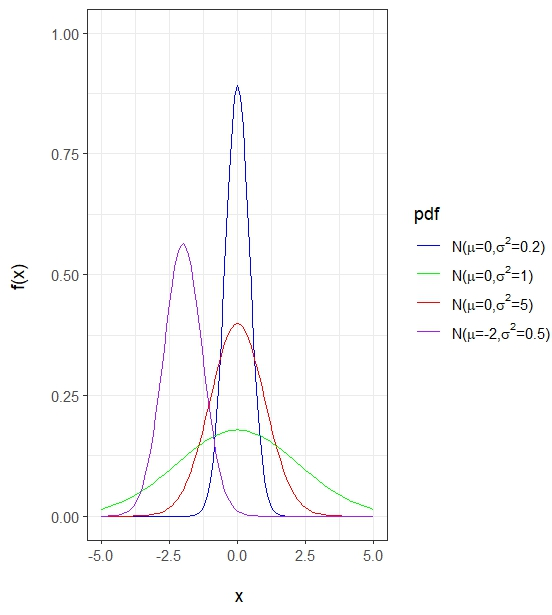
\includegraphics[scale=1]{Figuras/Normales.jpeg}
\caption{Distribuciones normales.}
\end{figure}

\begin{theorem}
Si $X$ tiene distribución $N(\mu ,\sigma ^{2})$, entonces
\begin{eqnarray*}
E(X) &=&\mu \\
V(X) &=&\sigma ^{2} \\
m_{X}(t) &=&e^{\mu t+\frac{(\sigma t)^{2}}{2}}
\end{eqnarray*}
\end{theorem}

Observaciones:
\begin{itemize}
\item La pdf de la v.a $X$, también se denota como: 
\begin{equation*}
\phi _{\mu,\sigma ^{2}}(x)=\frac{1}{\sqrt{2\pi \sigma ^{2}}}e^{-\frac{
(x-\mu )^{2}}{2\sigma ^{2}}}
\end{equation*}
\end{itemize}

\begin{itemize}
\item Si $\mu =0$ y $\sigma ^{2}=1$, entonces $X$ tiene distribución normal estándar:
\end{itemize}

\begin{equation*}
\phi _{\mu ,\sigma ^{2}}(x)=\phi (x)=\frac{1}{\sqrt{2\pi }}e^{-\frac{x^{2}}{2%
}}
\end{equation*}


\begin{itemize}
\item La función de distribución acumulativa (cdf) de una v.a $X$ con distribución $N(\mu ,\sigma ^{2})$, se denota con $\Phi _{\mu,\sigma ^{2}}(x)$, donde 
\begin{eqnarray*}
\Phi _{\mu ,\sigma ^{2}}(x) &=&F_{X}(x) \\
&=&P(X\leq x) \\
&=&\int_{-\infty }^{x}\frac{1}{\sqrt{2\pi \sigma ^{2}}}e^{-\frac{(u-\mu )^{2}%
}{2\sigma ^{2}}}du \\
&=&\int_{-\infty }^{x}\phi _{\mu ,\sigma ^{2}}(u)du
\end{eqnarray*}
\end{itemize}

Si $\mu =0$ y $\sigma ^{2}=1,$ entonces
\begin{equation*}
\Phi _{\mu ,\sigma ^{2}}(x)=\Phi (x)=\int_{-\infty }^{x}\phi (u)du
\end{equation*}

\begin{theorem}
Si $Z\sim N(0,1)$, entonces 
\begin{eqnarray*}
E(Z) &=&0 \\
V(Z) &=&1 \\
m_{Z}(t) &=&e^{t^{2}/2}
\end{eqnarray*}
\end{theorem} 

Demostración: 
\begin{eqnarray*}
E(Z) &=&\int_{-\infty }^{\infty }z\frac{1}{\sqrt{2\pi }}e^{-\frac{z^{2}}{2}
}dz \\
&=&\frac{1}{\sqrt{2\pi }}\int_{-\infty }^{\infty }ze^{-\frac{z^{2}}{2}}dz
\end{eqnarray*}

Sea $u=z^{2}/2$ entonces \ $du=zdz$

Luego
\begin{eqnarray*}
E(Z) &=&\frac{1}{\sqrt{2\pi }}\int_{-\infty }^{\infty }e^{-u}du \\
&=&\frac{1}{\sqrt{2\pi }}\left. e^{-\frac{z^{2}}{2}}\right\vert _{z=-\infty
}^{z=\infty } \\
&=&0
\end{eqnarray*}

Por otra parte 
\begin{eqnarray*}
E(Z^{2}) &=&\int_{-\infty }^{\infty }z^{2}\frac{1}{\sqrt{2\pi }}e^{-\frac{
z^{2}}{2}}dz \\
&=&\frac{1}{\sqrt{2\pi }}\int_{-\infty }^{\infty }zze^{-\frac{z^{2}}{2}}dz
\end{eqnarray*}

Considerando la integración por partes:
\begin{equation*}
\int uv^{\prime }=uv-\int u^{\prime }v
\end{equation*}
donde
\begin{eqnarray*}
u &=&z\text{ \ \ \ \ \ }v^{\prime }=ze^{-\frac{z^{2}}{2}} \\
du &=&dz\text{ \ \ \ }v=-e^{-\frac{z^{2}}{2}}
\end{eqnarray*}
Entonces%
\begin{eqnarray*}
E(Z^{2}) &=&\frac{1}{\sqrt{2\pi }}\int_{-\infty }^{\infty }zze^{-\frac{z^{2}
}{2}}dz \\
&=&\frac{1}{\sqrt{2\pi }}\left[ \left. -ze^{-\frac{z^{2}}{2}}\right\vert
_{z=-\infty }^{z=\infty }-\int_{-\infty }^{\infty }-e^{-\frac{z^{2}}{2}}dz
\right] \\
&=&\int_{-\infty }^{\infty }\frac{1}{\sqrt{2\pi }}e^{-\frac{z^{2}}{2}}dz%
\text{ \ \ \ //}Z\text{ es una pdf} \\
&=&1
\end{eqnarray*}
Luego 
\begin{eqnarray*}
V(Z) &=&E(Z^{2})-\left[ E(Z)\right] ^{2} \\
&=&1-0^{2} \\
&=&1
\end{eqnarray*}

Finalmente 
\begin{eqnarray*}
m_{Z}(t) &=&E(e^{tZ}) \\
&=&\int_{-\infty }^{\infty }e^{tz}\frac{1}{\sqrt{2\pi }}e^{-\frac{z^{2}}{2}
}dz \\
&=&\int_{-\infty }^{\infty }\frac{1}{\sqrt{2\pi }}e^{-\frac{z^{2}}{2}+tz}dz
\\
&=&\int_{-\infty }^{\infty }\frac{1}{\sqrt{2\pi }}e^{-\frac{1}{2}\left(
z^{2}-2tz+t^{2}-t^{2}\right) }dz \\
&=&\int_{-\infty }^{\infty }\frac{1}{\sqrt{2\pi }}e^{\frac{-1}{2}\left[
(z-t)^{2}-t^{2}\right] }dz \\
&=&\int_{-\infty }^{\infty }\frac{1}{\sqrt{2\pi }}e^{\frac{t^{2}}{2}}e^{%
\frac{-1}{2}(z-t)^{2}}dz \\
&=&e^{\frac{t^{2}}{2}}\int_{-\infty }^{\infty }\frac{1}{\sqrt{2\pi }}e^{%
\frac{-1}{2}(z-t)^{2}}dz\text{ //}Z\text{ es pdf} \\
&=&e^{\frac{t^{2}}{2}}
\end{eqnarray*}
Luego%
\begin{equation*}
m_{Z}(t)=e^{\frac{t^{2}}{2}}
\end{equation*}

\begin{teorem}
Si $X\sim N(\mu ,\sigma ^{2})$, entonces
\begin{eqnarray*}
E(X) &=&\mu \\
V(X) &=&\sigma ^{2} \\
m_{X}(t) &=&e^{\mu t+\frac{(\sigma t)^{2}}{2}}
\end{eqnarray*}
\end{teorem}
Demostración:

Sea 
\begin{equation*}
Z=\frac{X-\mu }{\sigma }
\end{equation*}

Note que $Z$ tiene distribución normal estándar, además

\begin{equation*}
X=\mu +\sigma Z
\end{equation*}
Luego%
\begin{eqnarray*}
E(X) &=&E(\mu +\sigma Z) \\
&=&\mu +\sigma E(Z)\text{ //Linealidad del operador} \\
&=&\mu +\sigma (0)\text{ //}Z\sim N(0,1)
\end{eqnarray*}%
i.e
\begin{equation*}
E(X)=\mu
\end{equation*}

Por otra parte 
\begin{eqnarray*}
E(X^{2}) &=&E\left[ (\mu +\sigma Z)^{2}\right] \\
&=&E\left[ \mu ^{2}+2\sigma Z+\sigma ^{2}Z^{2}\right] \\
&=&\mu ^{2}+2\sigma E(Z)+\sigma ^{2}E(Z^{2})\text{ //Linealidad del operador}
\\
&=&\mu ^{2}+\sigma ^{2}\text{ //}E(Z^{2})=1
\end{eqnarray*}

Entonces
\begin{equation*}
V(X)=\mu ^{2}+\sigma ^{2}-\mu ^{2}=\sigma ^{2}
\end{equation*}
Por lo tanto%
\begin{equation*}
V(X)=\sigma ^{2}
\end{equation*}

Finalmente%
\begin{eqnarray*}
m_{X}(t) &=&E(e^{tX}) \\
&=&E\left( e^{t(\mu +\sigma Z)}\right) \\
&=&e^{t\mu }E(e^{t\sigma Z})
\end{eqnarray*}
Como 
\begin{eqnarray*}
E(e^{t\sigma Z}) &=&\int_{-\infty }^{\infty }\frac{1}{\sqrt{2\pi }}e^{\frac{%
-1}{2}\left[ z^{2}-t\sigma z\right] }dz \\
&=&\int_{-\infty }^{\infty }\frac{1}{\sqrt{2\pi }}e^{\frac{-1}{2}\left[
(z-t\sigma )^{2}-t^{2}\sigma ^{2}\right] }dz \\
&=&\int_{-\infty }^{\infty }\frac{1}{\sqrt{2\pi }}e^{\frac{t^{2}\sigma ^{2}}{%
2}}e^{\frac{-1}{2}\left[ (z-t\sigma )^{2}\right] }dz \\
&=&e^{\frac{t^{2}\sigma ^{2}}{2}}\int_{-\infty }^{\infty }\frac{1}{\sqrt{%
2\pi }}e^{\frac{-1}{2}\left[ (z-t\sigma )^{2}\right] }dz \\
&=&e^{\frac{t^{2}\sigma ^{2}}{2}}
\end{eqnarray*}

Luego 
\begin{equation*}
m_{X}(t)=e^{t\mu +t^{2}\sigma ^{2}/2}
\end{equation*}

\begin{theorem}
Si $X\sim N(\mu ,\sigma ^{2})$ entonces
\begin{equation}
P(a<X<b)=\Phi \left( \frac{b-\mu }{\sigma }\right) -\Phi \left( \frac{a-\mu 
}{\sigma }\right)
\end{equation}
donde $a$, $b\in \mathbb{R}$.
\label{tem4}
\end{theorem}

Demostración:
\begin{equation*}
P(a<X<b)=\int_{a}^{b}\frac{1}{\sqrt{2\pi \sigma ^{2}}}e^{\frac{-1}{2}\left( 
\frac{x-\mu }{\sigma }\right) ^{2}}dx
\end{equation*}

Sea \ $z=\frac{x-\mu }{\sigma }$, entonces

\begin{equation*}
\begin{array}{lll}
P(a<X<b) & = & \int_{\frac{a-\mu }{\sigma }}^{\frac{b-\mu }{\sigma }}\frac{1
}{\sqrt{2\pi }}e^{\frac{-z^{2}}{2}}dx \\ 
& = & \int_{-\infty }^{\frac{b-\mu }{\sigma }}\frac{1}{\sqrt{2\pi }}e^{\frac{
-z^{2}}{2}}dx-\int_{-\infty }^{\frac{a-\mu }{\sigma }}\frac{1}{\sqrt{2\pi }}
e^{\frac{-z^{2}}{2}}dx \\ 
& = & \Phi \left( \frac{b-\mu }{\sigma }\right) -\Phi \left( \frac{a-\mu }{
\sigma }\right)
\end{array}
\end{equation*}
Por lo tanto 
\begin{equation*}
P(a<X<b)=\Phi \left( \frac{b-\mu }{\sigma }\right) -\Phi \left( \frac{a-\mu 
}{\sigma }\right)
\end{equation*}


La distribución normal tiene las siguientes características:

\begin{itemize}
    \item Simetría: Es simétrica alrededor de la media, lo que significa que las colas izquierda y derecha de la distribución son idénticas.
    \item Unimodal: Tiene un solo pico en la media.
    \item Forma de Campana: La función de densidad de probabilidad forma una curva en forma de campana.
    \item  Aproximadamente el 68\% de los datos caen dentro de una desviación estándar de la media, el 95\% dentro de dos desviaciones estándar y el 99.7\% dentro de tres desviaciones estándar.

\end{itemize}



%%%%%%%%%%%%%%%%%%%%%%%%%%%%%%%%%%%%%%%%%
\subsubsection{Resolución de problemas}

Para una variable aleatoria $X$, con distribución normal, $\mu=100$ y $sd=10$, calcular
$$
P(90 \leq X \leq 115)
$$
Esta probabilidad se puede calcular:
\begin{itemize}
    \item Integrando la pdf de la normal con $\mu=100$ y $sd=10$.
    \item Usando el Teorema (\ref{tem4}).
    \item Usando R.
\end{itemize}

\begin{figure}[h!]
\centering
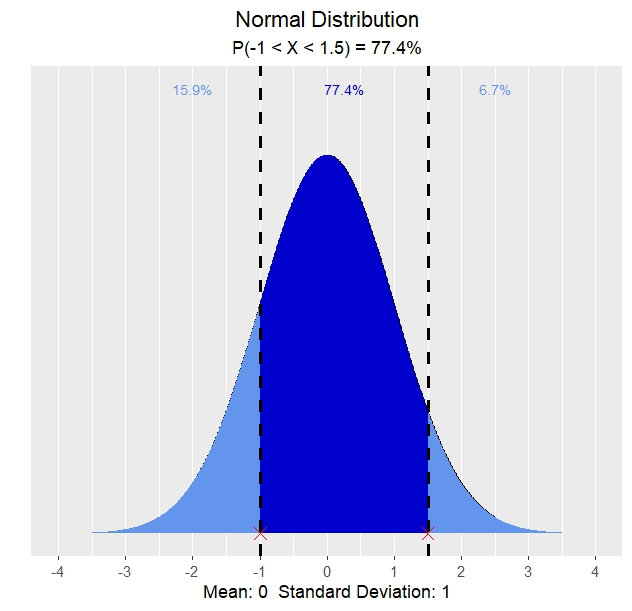
\includegraphics[scale=0.8]{Figuras/Normal_prob.jpeg}
\caption{Normal estándar.}
\end{figure}

Para una variable aleatoria $X$, con distribución normal, $\mu=100$ y $sd=10$, calcular
$$
P(X \leq 115)
$$
\begin{figure}[h!]
\centering
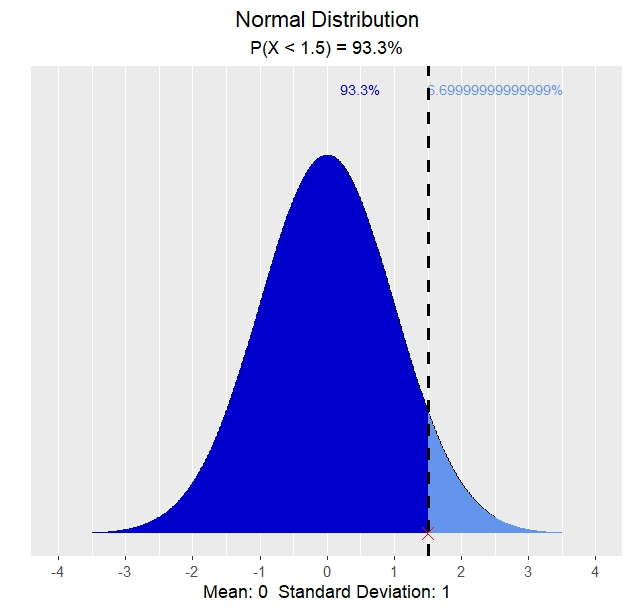
\includegraphics[scale=0.8]{Figuras/Normal2_prob.jpeg}
\caption{Normal estándar.}
\end{figure}


%%%%%%%%%%%%%%%%%%%%%%%%%%%%%%%%%%%%%%%%%
\subsubsection{Práctica con R}

Funciones para la distribución normal:
\begin{itemize}
\item dnorm(x, mean, sd), calcula $f(x)$
\item pnorm(q, mean, sd, lower.tail=TRUE),  calcula $P(X<q)$
\item qnorm(p, mean, sd, lower.tail=TRUE),  calcula $q$ tal que $P(X<q) = p$
\item rnorm(n, mean, sd), genera números aleatorios
\end{itemize}

\vspace{5mm}
Paquetes
\begin{lstlisting}
    library(vistributions)
    library(devtools)
\end{lstlisting}
\vspace{5mm}
Cálculo de 
$$
P(90 \leq X \leq 115)
$$
\begin{lstlisting}
      mu<-100
      sd<-10
      z1<-(90-mu)/sd
      z2<-(115-mu)/sd
      vdist_normal_prob(c(z1, z2),
                        mean =0, 
                        sd = 1,
                        type = 'both')
\end{lstlisting}

\vspace{5mm}
Cálculo de 
$$
P(90 \leq X \leq 115)
$$
\begin{lstlisting}
      p_sup <- pnorm(q=115, mean=100, sd=10)
      p_inf <- pnorm(q=90, mean=100, sd=10)
      p_sup - p_inf
\end{lstlisting}
\vspace{5mm}

Cálculo de
$$
P(X \leq 115)
$$
\begin{lstlisting}
      mu<-100
      sd<-10
      z2<-(115-mu)/sd;z2

      vdist_normal_prob(z2,
                        mean = 0,
                        sd = 1,
                        type ="lower")
\end{lstlisting}

\vspace{5mm}
Cálculo de
$$
P(X \leq 115)
$$
\begin{lstlisting}
      # pnorm() entrega la probabilidad de cola a izquierda.

      pnorm(q=115, mean=100, sd=10)
\end{lstlisting}

\vspace{5mm}
Cálculo de
$$
P(X \leq 115)
$$

\begin{lstlisting}
       mu<-100
       sd<-10
       var.x<-sd*sd

       pdf_normal <- function(x) 
             {
              (1/sqrt(2*pi*var.x))*exp(-(x-mu)^2/(2*var.x))
             }



        integrate(pdf_normal , lower=0, upper=115)
\end{lstlisting}

%%%%%%%%%%%%%%%%%%%%%%%%%%%%%%%%%%%%%%%%%
\subsection{Exponencial}

\begin{definition}
Una v.a $X$ tiene distribución Exponencial si su función densidad está dada por 
\begin{equation*}
f_{X}(x;\lambda )=\lambda e^{-\lambda x}I_{[0,\infty )}(x)
\end{equation*}
con $\lambda >0$. // $X\sim Exp(\lambda )$
\end{definition}

\begin{figure}[h!]
\centering
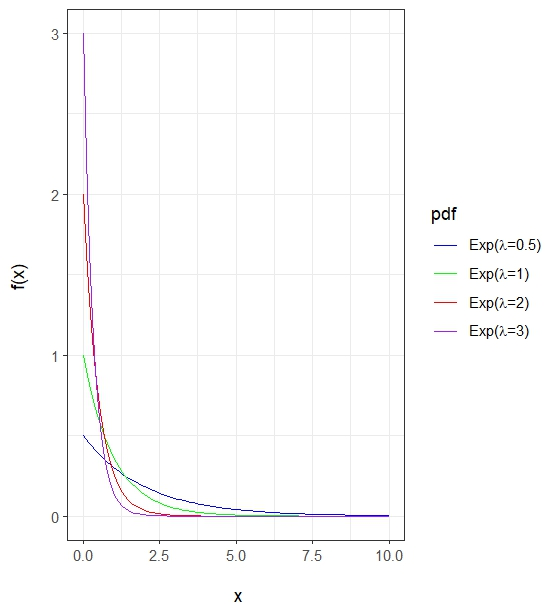
\includegraphics[scale=1]{Figuras/Exponenciales.jpeg}
\caption{Distribuciones exponenciales.}
\end{figure}


\begin{theorem}
 Si $X$ tiene distribución $Exp(\lambda)$, entonces
\begin{eqnarray*}
E(X) &=&\frac{1}{\lambda } \\
V(X) &=&\frac{1}{\lambda ^{2}} \\
m_{X}(t) &=&\frac{\lambda }{\lambda -t}\text{, }\lambda >t
\end{eqnarray*}
\end{theorem}

Demostración:
\begin{eqnarray*}
E(X) &=&\int_{-\infty }^{\infty }xf_{X}(x)dx \\
&=&\int_{0}^{\infty }x\lambda e^{-\lambda x}dx \\
&=&\lambda \int_{0}^{\infty }xe^{-\lambda x}dx
\end{eqnarray*}

Se efectúa una integración por partes: $\int uv^{\prime }=uv-\int u^{\prime }v$
\begin{eqnarray*}
u &=&x\text{ \ \ \ \ \ \ \ \ \ \ \ \ }du=dx \\
v^{\prime } &=&e^{-\lambda x}dx\text{ \ \ \ }v=-\frac{e^{-\lambda x}}{%
\lambda }
\end{eqnarray*}%
luego
\begin{eqnarray*}
E(X) &=&\lambda \left[ \left. \left( x\frac{\left( -e^{-\lambda x}\right) }{%
\lambda }\right) \right\vert _{0}^{\infty }-\int_{0}^{\infty }-\frac{%
e^{-\lambda x}}{\lambda }dx\right] \\
&=&\int_{0}^{\infty }e^{-\lambda x}dx
\end{eqnarray*}
sea 
\begin{equation*}
u=-\lambda x\text{ \ }du=-\lambda dx
\end{equation*}
\begin{eqnarray*}
E(X) &=&\int_{0}^{\infty }e^{-\lambda x}dx \\
&=&-\frac{1}{\lambda }\int_{0}^{\infty }e^{u}du \\
&=&-\frac{1}{\lambda }\left. e^{u}\right\vert _{0}^{\infty } \\
&=&-\frac{1}{\lambda }\left( 0-1\right) \\
&=&\frac{1}{\lambda }
\end{eqnarray*}

i.e
\begin{equation*}
E(X)=\frac{1}{\lambda }
\end{equation*}

Por otra parte, como 
\begin{equation*}
V(X)=E(X^{2})-\left[ E(X)\right] ^{2}
\end{equation*}

Entonces
\begin{eqnarray*}
E(X^{2}) &=&\int_{-\infty }^{\infty }x^{2}f_{X}(x)dx \\
&=&\int_{0}^{\infty }x^{2}\lambda e^{-\lambda x}dx \\
&=&\lambda \int_{0}^{\infty }x^{2}e^{-\lambda x}dx
\end{eqnarray*}

Realizando una integración por partes: $\int uv^{\prime }=uv-\int u^{\prime }v$

\begin{eqnarray*}
u &=&x^{2}\text{ \ \ \ \ \ \ \ \ \ \ \ \ }\frac{du}{dx}=2x \\
dv &=&e^{-\lambda x}dx\text{ \ \ \ \ \ \ \ \ }v=-\frac{e^{-\lambda x}}{\lambda}
\end{eqnarray*}
Entonces
\begin{eqnarray*}
E(X^{2}) &=&\left. \left( -\lambda x^{2}\frac{e^{-\lambda x}}{\lambda }
\right) \right\vert _{0}^{\infty }-\lambda \int_{0}^{\infty }-\frac{
e^{-\lambda x}}{\lambda }2xdx \\
&=&\int_{0}^{\infty }e^{-\lambda x}2xdx \\
&=&2\int_{0}^{\infty }xe^{-\lambda x}dx \\
&=&\frac{2}{\lambda }\int_{0}^{\infty }\lambda xe^{-\lambda x}dx
\end{eqnarray*}

Note que
\begin{equation*}
\int_{0}^{\infty }\lambda xe^{-\lambda x}dx=E(X)=1/\lambda
\end{equation*}

Entonces, sustituyendo
\begin{eqnarray*}
E(X^{2}) &=&\frac{2}{\lambda }\cdot \frac{1}{\lambda } \\
&=&\frac{2}{\lambda ^{2}}
\end{eqnarray*}

Luego 
\begin{eqnarray*}
V(X) &=&E(X^{2})-\left[ E(X)\right] ^{2} \\
&=&\frac{2}{\lambda ^{2}}-\frac{1}{\lambda ^{2}} \\
&=&\frac{1}{\lambda ^{2}}
\end{eqnarray*}

Finalmente 
\begin{eqnarray*}
m_{X}(t) &=&E(e^{tX}) \\
&=&\int_{0}^{\infty }e^{tx}\lambda e^{-\lambda x}dx \\
&=&\int_{0}^{\infty }\lambda e^{tx}e^{-\lambda x}dx \\
&=&\lambda \int_{0}^{\infty }e^{-x(\lambda -t)}dx \\
&=&\frac{\lambda }{\lambda -t}\int_{0}^{\infty }\left( \lambda -t\right)
e^{-x(\lambda -t)}dx\text{ // }\lambda -t>0, \\
&=&\frac{\lambda }{\lambda -t}
\end{eqnarray*}
Por lo tanto 
\begin{equation*}
m_{X}(t)=\frac{\lambda }{\lambda -t}.
\end{equation*}

Una segunda parametrización para la pdf exponencial (Casella, 1990), está dada por
\begin{equation*}
f(x)=\frac{1}{\lambda }e^{-\frac{x}{\lambda }}I_{(0,\infty )}(x)
\end{equation*}%
donde $\lambda >0.$ En este caso 
\begin{eqnarray*}
E(X) &=&\lambda \\
V(X) &=&\lambda ^{2} \\
m_{X}(t) &=&\frac{1}{1-\lambda t}\text{, }\frac{1}{\lambda }>t
\end{eqnarray*}

\textbf{Tarea}: Demostrarlo.



%%%%%%%%%%%%%%%%%%%%%%%%%%%%%%%%%%%
\subsection{Gamma}


\begin{definition}
Una v.a $X$ tiene distribución Gamma($r,\lambda $) si su pdf está dada por 
\begin{equation*}
f(x;r,\lambda )=\frac{\lambda }{\Gamma (r)}\left( \lambda x\right)
^{r-1}e^{-\lambda x}I_{[0,\infty )}(x)
\end{equation*}
con $r,\lambda >0.$
\end{definition}

\begin{figure}[h!]
\centering
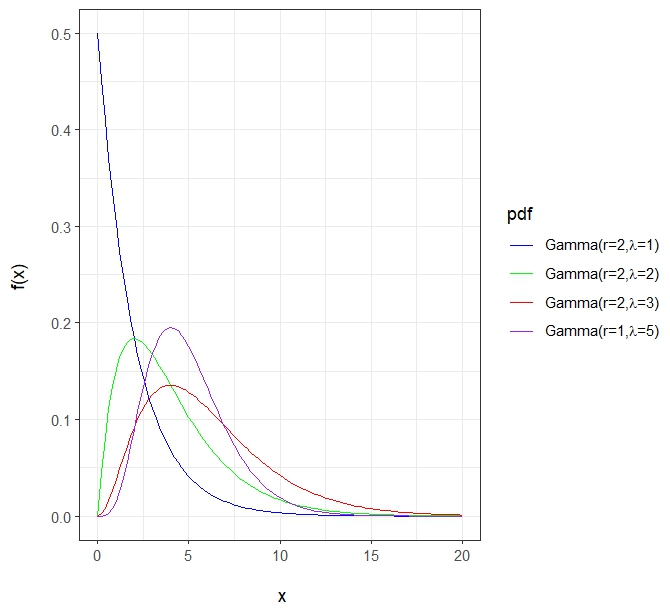
\includegraphics[scale=1]{Figuras/Gammas.jpeg}
\caption{Distribuciones Gammas.}
\end{figure}

\begin{theorem}
Si $X$ tiene distribución Gamma($r,\lambda$), entonces
\begin{eqnarray*}
E(X) &=&\frac{r}{\lambda } \\
V(X) &=&\frac{r}{\lambda ^{2}} \\
m_{X}(t) &=&\left( \frac{\lambda }{\lambda -t}\right) ^{r}\text{, \ }t\leq
\lambda
\end{eqnarray*}
\end{theorem}


Demostración
\begin{eqnarray*}
E(X) &=&\int_{0}^{\infty }x\frac{\lambda }{\Gamma (r)}\left( \lambda
x\right) ^{r-1}e^{-\lambda x}dx \\
&=&\int_{0}^{\infty }x\frac{\lambda }{\Gamma (r)}\lambda
^{r-1}x^{r-1}e^{-\lambda x}dx \\
&=&\int_{0}^{\infty }\frac{\lambda ^{r}}{\Gamma (r)}x^{r}e^{-\lambda x}dx \\
&=&\frac{\lambda ^{r}}{\Gamma (r)}\int_{0}^{\infty }x^{r}e^{-\lambda x}dx
\end{eqnarray*}

Realizando integración por partes: $\int uv^{\prime }=uv-\int u^{\prime}v$
\begin{equation*}
\begin{array}{ccc}
u=x^{r} &  & v^{\prime }=e^{-\lambda x} \\ 
\frac{du}{dx}=rx^{r-1} &  & v=\frac{-e^{-\lambda x}}{\lambda }
\end{array}
\end{equation*}

Entonces
\begin{eqnarray*}
E(X) &=&\frac{\lambda ^{r}}{\Gamma (r)}\int_{0}^{\infty }x^{r}e^{-\lambda
x}dx \\
&=&\left. \frac{\lambda ^{r}}{\Gamma (r)}x^{r}\left( -\frac{e^{-\lambda x}}{%
\lambda }\right) \right\vert _{x=0}^{x=\infty }-\frac{\lambda ^{r}}{\Gamma
(r)}\int_{0}^{\infty }rx^{r-1}\left( \frac{-e^{-\lambda x}}{\lambda }\right)
dx \\
&=&\int_{0}^{\infty }\frac{\lambda }{\Gamma (r)}\lambda ^{r-1}rx^{r-1}\left( 
\frac{e^{-\lambda x}}{\lambda }\right) dx \\
&=&\frac{r}{\lambda }\int_{0}^{\infty }\frac{\lambda }{\Gamma (r)}\lambda
^{r-1}x^{r-1}e^{-\lambda x}dx \\
&=&\frac{r}{\lambda }\int_{0}^{\infty }\frac{\lambda }{\Gamma (r)}(\lambda
x)^{r-1}e^{-\lambda x}dx\text{ \ // pdf gamma} \\
&=&\frac{r}{\lambda }
\end{eqnarray*}

Luego
\begin{equation*}
E(X)=\frac{r}{\lambda }
\end{equation*}

Por otra, parte, 
\begin{equation*}
V(X)=E(X^{2})-[E(X)]^{2}
\end{equation*}

entonces
\begin{eqnarray*}
E(X^{2}) &=&\int_{0}^{\infty }x^{2}\frac{\lambda }{\Gamma (r)}\lambda
^{r-1}x^{r-1}e^{-\lambda x}dx \\
&=&\int_{0}^{\infty }\frac{\lambda }{\Gamma (r)}\lambda
^{r-1}x^{r+1}e^{-\lambda x}dx \\
&=&\int_{0}^{\infty }\frac{\lambda ^{r}}{\Gamma (r)}x^{r+1}e^{-\lambda x}dx
\\
&=&\frac{\lambda ^{r}}{\Gamma (r)}\int_{0}^{\infty }x^{r+1}e^{-\lambda x}dx
\end{eqnarray*}

Realizando integración por partes: $\int uv^{\prime }=uv-\int u^{\prime}v$

$u=x^{r+1}$,  $v^{\prime }=e^{-\lambda x}$

$\frac{du}{dx}=(r+1)x^{r}$  $v=\frac{-e^{-\lambda x}}{\lambda}$

Entonces
\begin{eqnarray*}
E(X^{2}) &=&\frac{\lambda ^{r}}{\Gamma (r)}\int_{0}^{\infty
}x^{r+1}e^{-\lambda x}dx \\
&=&\left. \frac{\lambda ^{r}}{\Gamma (r)}x^{r+1}\left( \frac{-e^{-\lambda x}%
}{\lambda }\right) \right\vert _{x=0}^{x=\infty }-\frac{\lambda ^{r}}{\Gamma
(r)}\int_{0}^{\infty }(r+1)x^{r}\left( \frac{-e^{-\lambda x}}{\lambda }%
\right) dx \\
&=&\frac{\lambda ^{r}}{\Gamma (r)}\int_{0}^{\infty }(r+1)x^{r}\frac{%
e^{-\lambda x}}{\lambda }dx \\
&=&\frac{(r+1)}{\lambda }\int_{0}^{\infty }\frac{\lambda ^{r}}{\Gamma (r)}%
x^{r}e^{-\lambda x}dx \\
&=&\frac{(r+1)}{\lambda }\int_{0}^{\infty }\frac{\lambda }{\Gamma (r)}%
\lambda ^{r-1}x^{r}e^{-\lambda x}dx
\end{eqnarray*}
Note que 
\begin{equation*}
E(X)=\int_{0}^{\infty }\frac{\lambda }{\Gamma (r)}\lambda
^{r-1}x^{r}e^{-\lambda x}dx=\frac{r}{\lambda }
\end{equation*}
Sustituyendo%
\begin{eqnarray*}
E(X^{2}) &=&\frac{(r+1)}{\lambda }\cdot \frac{r}{\lambda } \\
&=&\frac{r(r+1)}{\lambda ^{2}}
\end{eqnarray*}

Entonces
\begin{eqnarray*}
V(X) &=&E(X^{2})-\left[ E(X)\right] ^{2} \\
&=&\frac{r^{2}+r}{\lambda ^{2}}-\frac{r^{2}}{\lambda ^{2}}\text{ } \\
&=&\frac{r}{\lambda ^{2}}
\end{eqnarray*}

Por otra parte 
\begin{eqnarray*}
m_{X}(t) &=&E(e^{tX}) \\
&=&\int_{0}^{\infty }e^{tx}\frac{\lambda }{\Gamma (r)}\left( \lambda
x\right) ^{r-1}e^{-\lambda x}dx \\
&=&\int_{0}^{\infty }\frac{\lambda }{\Gamma (r)}(\lambda
x)^{r-1}e^{-(\lambda -t)x}dx \\
&=&\int_{0}^{\infty }\frac{\lambda }{\Gamma (r)}\lambda
^{r-1}x^{r-1}e^{-(\lambda -t)x}dx \\
&=&\int_{0}^{\infty }\frac{\lambda ^{r}}{\Gamma (r)}x^{r-1}e^{-(\lambda
-t)x}dx \\
&=&\frac{\lambda ^{r}}{(\lambda -t)^{r}}\int_{0}^{\infty }\frac{(\lambda
-t)^{r}}{\Gamma (r)}x^{r-1}e^{-(\lambda -t)x}dx \\
&=&=\frac{\lambda ^{r}}{(\lambda -t)^{r}}\int_{0}^{\infty }\frac{(\lambda -t)%
}{\Gamma (r)}(\lambda -t)^{r-1}x^{r-1}e^{-(\lambda -t)x}dx \\
&=&\frac{\lambda ^{r}}{(\lambda -t)^{r}}\int_{0}^{\infty }\frac{(\lambda -t)%
}{\Gamma (r)}\left[ (\lambda -t)x\right] ^{r-1}e^{-(\lambda -t)x}dx\text{ }
\end{eqnarray*}

Note que 
\begin{equation*}
\int_{0}^{\infty }\frac{(\lambda -t)}{\Gamma (r)}\left[ (\lambda -t)x\right]
^{r-1}e^{-(\lambda -t)x}dx
\end{equation*}%
es la pdf de una Gamma($r,(\lambda -t)$), donde $\lambda -t>0$ ($\lambda >0,$
$\left\vert h\right\vert <t,$ $h>0$) es decir $\lambda >t.$ Entonces 
\begin{equation*}
\int_{0}^{\infty }\frac{(\lambda -t)}{\Gamma (r)}\left[ (\lambda -t)x\right]
^{r-1}e^{-(\lambda -t)x}dx=1
\end{equation*}

Luego
\begin{equation*}
m_{X}(t)=\frac{\lambda ^{r}}{(\lambda -t)^{r}}=\left( \frac{\lambda }{%
\lambda -t}\right) ^{r}\text{, \ }t<\lambda
\end{equation*}

Por lo tanto, 
\begin{equation*}
m_{X}(t)=\left( \frac{\lambda }{\lambda -t}\right) ^{r}\text{, \ }t<\lambda
\end{equation*}

Una segunda parametrización para la pdf de una Gamma, está dada por (Casella, $1990$) 
\begin{equation*}
f(x,r,\lambda )=\frac{1}{\Gamma (r)\lambda ^{r}}x^{r-1}e^{-x/\lambda
}I_{(0,\infty )}(x)
\end{equation*}

Donde
\begin{eqnarray*}
E(X) &=&r\lambda \\
V(X) &=&r\lambda ^{2} \\
m_{X}(t) &=&\left( \frac{1}{1-\lambda t}\right) ^{r}\text{, }t<\frac{1}{%
\lambda }
\end{eqnarray*}


\textbf{Tarea}: Demostrarlo.

%%%%%%%%%%%%%%%%%%%%%%%%%%%%%%%%%%
\subsection{Chi cuadrada}

\begin{definition}
La  pdf de la $\chi^2$ está dada por
$$
f(x)=\frac{1}{\Gamma(k/2)}\left(\frac{1}{2}\right)^{k/2}x^{k/2-1}e^{-(1/2)x}I_{(0,\infty)}(x)
$$    
$k=1,2,...$, $0\leq x\leq \infty $
\end{definition}

\begin{figure}[h!]
\centering
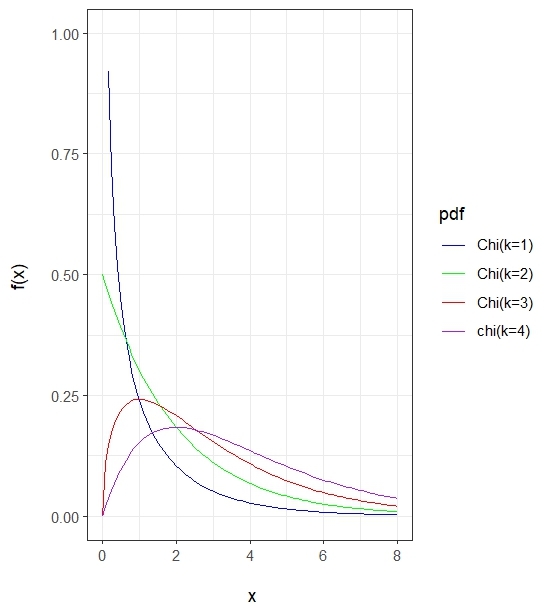
\includegraphics[scale=1]{Figuras/Chi_cuadradas.jpeg}
\caption{Distribución Chi cuadrada.}
\end{figure}

\begin{theorem}
Si $X$ tiene distribución $\chi^2$ con $k$ grados de libertad, entonces

\begin{eqnarray*}
E(X) &=&k \\
V(X) &=&2k \\
m_{X}(t) &=&\left( \frac{1 }{1 -2t}\right)^{k/2}\text{, \ }t\leq 1/2
\end{eqnarray*}
\end{theorem}


%%%%%%%%%%%%%%%%%%%%%%%%%%%%%%%%%%
\subsection{Beta}

\begin{definition}
Una v.a $X$ tiene distribución $Beta(a,b)$ si su función densidad está dada por 
\begin{equation*}
f(x;a,b)=\frac{1}{B(a,b)}x^{a-1}(1-x)^{b-1}I_{(0,1)}(x)
\end{equation*}
con $a,b>0.$ \ //$X\sim Beta(a,b)$
\end{definition}

\begin{figure}[h!]
\centering
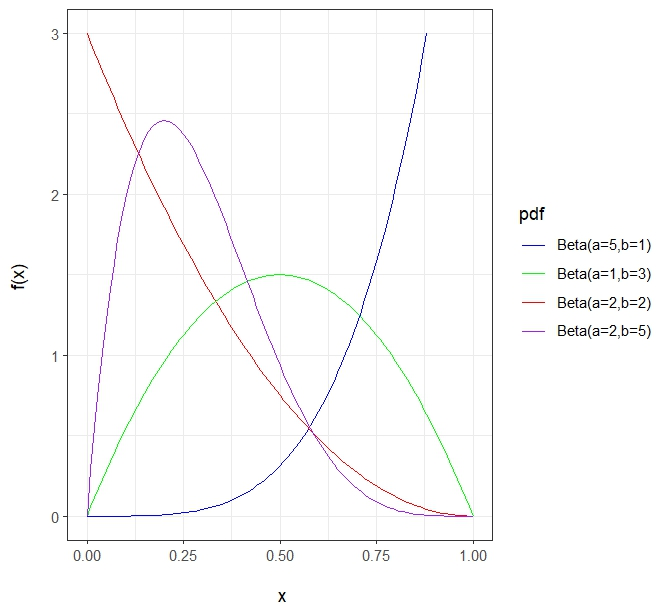
\includegraphics[scale=1]{Figuras/Betas.jpeg}
\caption{Distribuciones Betas.}
\end{figure}

\begin{definition}
A la función
\begin{equation*}
B(a,b)=\int_{0}^{1}x^{a-1}(1-x)^{b-1}dx
\end{equation*}
se le llama función beta, y tiene las siguientes propiedades: 
\begin{eqnarray*}
B(a,b) &=&\frac{\Gamma (a)\Gamma (b)}{\Gamma (a+b)} \\
B(a,b) &=&B(b,a)
\end{eqnarray*}
\end{definition}

\begin{figure}[h!]
\centering
\includegraphics[scale=1]{Figuras/Beta.jpeg}
\caption{Distribución Beta.}
\end{figure}


\begin{theorem}
Si $X$ tiene distribución Beta($a$, $b$), entonces
\begin{eqnarray*}
E(X) &=&\frac{a}{a+b} \\
V(X) &=&\frac{ab}{(a+b+1)(a+b)^{2}} \\
m_{X}(t) &=&1+\sum_{k=1}^{\infty }\frac{t^{k}}{k!}\left(
\prod\limits_{r=0}^{k-1}\frac{a+r}{a+b+r}\right)
\end{eqnarray*}
\end{theorem}

Demostración:
\begin{eqnarray*}
E(X^{k}) &=&\int_{0}^{1}x^{k}\frac{1}{B(a,b)}x^{a-1}(1-x)^{b-1}dx \\
&=&\frac{1}{B(a,b)}\int_{0}^{1}x^{k+a-1}(1-x)^{b-1}dx\text{ \ }//\text{Def.}
\\
&=&\frac{B(k+a,b)}{B(a,b)} \\
&=&\frac{\Gamma (k+a)\Gamma (b)/\Gamma (k+a+b)}{\Gamma (a)\Gamma (b)/\Gamma
(a+b)} \\
&=&\frac{\Gamma (a+b)\Gamma (k+a)\Gamma (b)}{\Gamma (k+a+b)\Gamma (a)\Gamma
(b)} \\
&=&\frac{\Gamma (a+b)\Gamma (k+a)}{\Gamma (a)\Gamma (k+a+b)}
\end{eqnarray*}

Luego 
\begin{equation*}
E(X^{k})=\frac{\Gamma (a+b)\Gamma (k+a)}{\Gamma (a)\Gamma (k+a+b)}
\end{equation*}


Por otra parte (Mood, pag. $534$),

\begin{equation*}
\Gamma (r)=\int_{0}^{\infty }x^{r-1}e^{-x}dx
\end{equation*}%
entonces 
\begin{equation*}
\Gamma (r+1)=\int_{0}^{\infty }x^{r}e^{-x}dx
\end{equation*}

Note que 
\begin{equation*}
\Gamma (r+1)=r\Gamma (r)
\end{equation*}

Lo cual se puede justificar de la siguiente manera: Realizando integración por partes: $\int uv^{\prime }=uv-\int u^{\prime }v$

$u=x^{r}$ \ \ \ \ \ \ \ \ \ \ $v^{\prime }=e^{-x}$

$\frac{du}{dx}=rx^{r-1}$ \ \ \ $v=-e^{-x}$

\begin{eqnarray*}
\Gamma (r+1) &=&\left. x^{r}(-e^{-x})\right\vert _{0}^{\infty
}-\int_{0}^{\infty }rx^{r-1}(-e^{-x})dx \\
&=&r\int_{0}^{\infty }x^{r-1}e^{-x}dx\text{ \ //}\Gamma (t)=\int_{0}^{\infty
}x^{t-1}e^{-x}dx \\
&=&r\Gamma (r)
\end{eqnarray*}
es decir 
\begin{equation*}
\Gamma (r+1)=r\Gamma (r)
\end{equation*}


Para $k=1$ en 
\begin{equation*}
E(X^{k})=\frac{\Gamma (a+b)\Gamma (k+a)}{\Gamma (a)\Gamma (k+a+b)}
\end{equation*}%
se tiene que

\begin{eqnarray*}
E(X) &=&\frac{\Gamma (a+b)\Gamma (1+a)}{\Gamma (a)\Gamma (1+a+b)}\text{ \ // 
}\Gamma (r+1)=r\Gamma (r) \\
&=&\frac{\Gamma (a+b)a\Gamma (a)}{\Gamma (a)(a+b)\Gamma (a+b)} \\
&=&\frac{a}{a+b}
\end{eqnarray*}

Entonces 
\begin{equation*}
E(X)=\frac{a}{a+b}
\end{equation*}

Para $k=2$ en
\begin{equation*}
E(X^{k})=\frac{\Gamma (a+b)\Gamma (k+a)}{\Gamma (a)\Gamma (k+a+b)}
\end{equation*}

se tiene lo siguiente
\begin{eqnarray*}
E(X^{2}) &=&\frac{\Gamma (a+b)\Gamma (2+a)}{\Gamma (a)\Gamma (2+a+b)} \\
&=&\frac{\Gamma (a+b)\Gamma (1+(1+a))}{\Gamma (a)\Gamma (1+(1+a+b))}\text{ \
\ \ // }\Gamma (r+1)=r\Gamma (r) \\
&=&\frac{\Gamma (a+b)(a+1)\Gamma (a+1)}{\Gamma (a)(1+a+b)\Gamma (1+a+b)}%
\text{ \ \ // }\Gamma (r+1)=r\Gamma (r) \\
&=&\frac{\Gamma (a+b)(a+1)a\Gamma (a)}{\Gamma (a)(1+a+b)(a+b)\Gamma (a+b)}%
\text{ } \\
&=&\frac{a(a+1)}{(a+b)(1+a+b)}
\end{eqnarray*}

Luego 
\begin{eqnarray*}
V(X) &=&E(X^{2})-[E(X)]^{2} \\
&=&\frac{a(a+1)}{(a+b)(1+a+b)}-\frac{a^{2}}{(a+b)^{2}} \\
&=&\frac{(a+b)(a^{2}+a)-a^{2}(1+a+b)}{(1+a+b)(a+b)^{2}} \\
&=&\frac{a^{3}+ab^{2}+a^{2}+ab-a^{2}-a^{3}-a^{2}b}{(1+a+b)(a+b)^{2}} \\
&=&\frac{ab}{(1+a+b)(a+b)^{2}}
\end{eqnarray*}
es decir,
\begin{equation*}
V(X)=\frac{ab}{(1+a+b)(a+b)^{2}}
\end{equation*}

Finalmente 
\begin{eqnarray*}
m_{X}(t) &=&E(e^{tX}) \\
&=&\int_{0}^{1}\frac{e^{tx}}{B(a,b)}x^{a-1}(1-x)^{b-1}dx \\
&=&\frac{1}{B(a,b)}\int_{0}^{1}\sum_{k=0}^{\infty }\frac{(tx)^{k}}{k!}%
x^{a-1}(1-x)^{b-1}dx \\
&=&\frac{1}{B(a,b)}\int_{0}^{1}\sum_{k=0}^{\infty }\frac{t^{k}x^{k}}{k!}%
x^{a-1}(1-x)^{b-1}dx \\
&=&\frac{1}{B(a,b)}\sum_{k=0}^{\infty }\frac{t^{k}}{k!}%
\int_{0}^{1}x^{k}x^{a-1}(1-x)^{b-1}dx \\
&=&\frac{1}{B(a,b)}\sum_{k=0}^{\infty }\frac{t^{k}}{k!}\int_{0}^{1}\frac{%
B(a+k,b)}{B(a+k,b)}x^{k+a-1}(1-x)^{b-1}dx\text{ } \\
&=&\frac{1}{B(a,b)}\sum_{k=0}^{\infty }\frac{t^{k}}{k!}B(a+k,b)\int_{0}^{1}%
\frac{1}{B(a+k,b)}x^{k+a-1}(1-x)^{b-1}dx\text{ //pdf} \\
&=&\sum_{k=0}^{\infty }\frac{t^{k}}{k!}\frac{B(a+k,b)}{B(a,b)} \\
&=&\sum_{k=0}^{\infty }\frac{t^{k}}{k!}\left[ \left. \frac{\Gamma
(a+k)\Gamma (b)}{\Gamma (a+b+k)}\right/ \frac{\Gamma (a)\Gamma (b)}{\Gamma
(a+b)}\right] \text{ \ \ //}B(a,b)=\frac{\Gamma (a)\Gamma (b)}{\Gamma (a+b)}
\\
&=&\sum_{k=0}^{\infty }\frac{t^{k}}{k!}\left[ \frac{\Gamma (a+b)\Gamma
(a+k)\Gamma (b)}{\Gamma (a+b+k)\Gamma (a)\Gamma (b)}\right] \\
&=&\sum_{k=0}^{\infty }\frac{t^{k}}{k!}\left[ \frac{\Gamma (a+b)\Gamma (a+k)%
}{\Gamma (a)\Gamma (a+b+k)}\right] \text{ } \\
&=&1+\sum_{k=1}^{\infty }\frac{t^{k}}{k!}\left[ \frac{\Gamma (a+b)\Gamma
(a+k)}{\Gamma (a)\Gamma (a+b+k)}\right] \\
&=&1+\sum_{k=1}^{\infty }\frac{t^{k}}{k!}\left[ \frac{\Gamma (a+b)\Gamma
(a)\prod\limits_{r=0}^{k-1}(a+r)}{\Gamma (a)\Gamma
(a+b)\prod\limits_{r=0}^{k-1}(a+b+r)}\right] \text{ } \\
&=&1+\sum_{k=1}^{\infty }\frac{t^{k}}{k!}\left[ \prod\limits_{r=0}^{k-1}%
\frac{a+r}{a+b+r}\right] \text{ }
\end{eqnarray*}

Luego
\begin{equation*}
m_{X}(t)=1+\sum_{k=1}^{\infty }\frac{t^{k}}{k!}\left[ \prod%
\limits_{r=0}^{k-1}\frac{a+r}{a+b+r}\right] \text{ }
\end{equation*}


%%%%%%%%%%%%%%%%%%%%%%%%%%%%%%%%%%
\subsection{Cauchy}

\begin{definition}
Una v.a $X$ tiene distribución Cauchy si su función densidad está dada por 
\begin{equation*}
f(x;\alpha ,\beta )=\frac{1}{\pi \beta \left[ 1+\left( \frac{x-\alpha }{%
\beta }\right) ^{2}\right] }I_{(-\infty ,\infty )}(x)
\end{equation*}
$-\infty <\alpha <\infty ,$ $\beta >0.$ // $X\sim Cauchy(\alpha ,\beta )$
\end{definition}


\begin{figure}[h!]
\centering
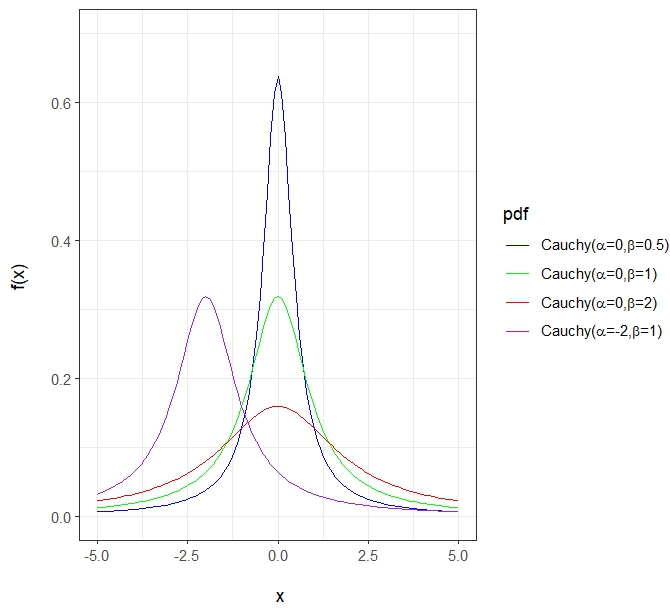
\includegraphics[scale=1]{Figuras/Cauchys.jpeg}
\caption{Distribuciones Cauchy.}
\end{figure}

\begin{theorem}
Si $X$ tiene distribución $Cauchy(\alpha ,\beta )$, entonces
\begin{equation*}
\begin{array}{l}
E(X)\text{ no existe} \\ 
V(X)\text{ no existe} \\ 
\text{La fgm no existe}
\end{array}
\end{equation*}
\end{theorem}

Veamos lo que pasa con la $E(X)$.
\begin{eqnarray*}
E(X) &=&\int_{-\infty }^{\infty }\frac{x}{\pi \beta \left[ 1+\left( \frac{%
x-\alpha }{\beta }\right) ^{2}\right] }dx \\
&=&\frac{1}{\pi \beta }\int_{-\infty }^{\infty }\frac{x}{\left[ 1+\frac{1}{%
\beta ^{2}}\left( x-\alpha \right) ^{2}\right] }dx \\
&=&\frac{1}{\pi \beta }\int_{-\infty }^{\infty }\frac{x}{\left[ \frac{\beta
^{2}+\left( x-\alpha \right) ^{2}}{\beta ^{2}}\right] }dx \\
&=&\frac{1}{\pi \beta }\int_{-\infty }^{\infty }\beta ^{2}\frac{x}{\beta
^{2}+(x-\alpha )^{2}}dx \\
&=&\frac{\beta }{\pi }\int_{-\infty }^{\infty }\frac{x}{\beta ^{2}+(x-\alpha
)^{2}}dx \\
&=&\frac{\beta }{\pi }\int_{-\infty }^{\infty }\frac{\alpha }{\beta
^{2}+(x-\alpha )^{2}}dx+\frac{\beta }{2\pi }\int_{-\infty }^{\infty }\frac{%
2(x-\alpha )}{\beta ^{2}+(x-\alpha )^{2}}dx
\end{eqnarray*}


En cuanto a la primera integral, se tiene que
\begin{eqnarray*}
\frac{\beta }{\pi }\int_{-\infty }^{\infty }\frac{\alpha }{\beta
^{2}+(x-\alpha )^{2}}dx &=&\frac{\beta \alpha }{\pi }\int_{-\infty }^{\infty
}\frac{dx}{\beta ^{2}+(x-\alpha )^{2}} \\
&=&\frac{\beta \alpha }{\pi }\int_{-\infty }^{\infty }\frac{dx/\beta ^{2}}{%
\left( \beta ^{2}+(x-\alpha )^{2}\right) /\beta ^{2}} \\
&=&\frac{\alpha }{\beta \pi }\int_{-\infty }^{\infty }\frac{dx}{1+(\frac{%
x-\alpha }{\beta })^{2}}\text{ //}\left( \arctan x\right) ^{\prime
}=1/(1+x^{2}) \\
&=&\frac{\alpha }{\beta \pi }\left. \arctan \left( \frac{x-\alpha }{\beta }%
\right) \right\vert _{-\infty }^{\infty } \\
&=&\frac{\alpha }{\beta \pi }\left( \frac{\pi }{2}-\left( -\frac{\pi }{2}%
\right) \right) = \\
&=&\frac{\alpha }{\beta \pi }\frac{2\pi }{2} \\
&=&\frac{\alpha }{\beta }
\end{eqnarray*}

Luego
\begin{eqnarray*}
E(X) &=&\frac{\beta }{\pi }\int_{-\infty }^{\infty }\frac{\alpha }{\beta
^{2}+(x-\alpha )^{2}}dx+\frac{\beta }{2\pi }\int_{-\infty }^{\infty }\frac{%
2(x-\alpha )}{\beta ^{2}+(x-\alpha )^{2}}dx \\
&=&\frac{\alpha }{\beta }+\frac{\beta }{2\pi }\int_{-\infty }^{\infty }\frac{%
2(x-\alpha )}{\beta ^{2}+(x-\alpha )^{2}}dx\text{ \ //}\frac{d}{dx}\ln
(f(x))=\frac{f{\acute{}}^{\prime }(x)}{f(x)} \\
&=&\frac{\alpha }{\beta }+\frac{\beta }{2\pi }\left. \ln \left[ \beta
^{2}+(x-\alpha )^{2}\right] \right\vert _{-\infty }^{\infty }
\end{eqnarray*}

Note que 
\begin{equation*}
\left. \ln \left[ \beta ^{2}+(x-\alpha )^{2}\right] \right\vert _{-\infty
}^{\infty }
\end{equation*}%
diverge cuando $x\rightarrow \infty $ ya que si $\ln (x)_{x\rightarrow
\infty }=\infty $ \ entonces\ $\ln (x^{2})_{x\rightarrow \infty }=\infty$.
Lo mismo pasa para cuando y $x\rightarrow -\infty $.
Por lo tanto $E(X)$ no existe.

Por otra parte $V(X)$ tampoco existe ya que $V(X)=E(X^{2})-\left[ E(X)\right]^{2}$ donde $E(X)$ no existe.

Finalmente la fgm de $X,$ que está dada por 
\begin{equation*}
m_{X}(t)=E(e^{tX})=\int_{-\infty }^{\infty }\frac{e^{tx}}{\pi \beta \left[
1+\left( \frac{x-\alpha }{\beta }\right) ^{2}\right] }dx
\end{equation*}%
no existe (\textbf{Tarea}).

Observación:
\begin{itemize}
\item Cuando la fgm no existe, entonces se puede utilizar la función
característica 
\begin{equation*}
\phi (t)=E(e^{itX})\text{, }-\infty <t<\infty
\end{equation*}%
donde $i=\sqrt{-1}$, la cual siempre existe y determina de manera única
la distribución de \ la v.a $X.$

\item Si la v.a $X$ tiene $n$-ésimo momento finito, entonces 
\begin{equation*}
\left. \frac{d^{n}}{dt^{n}}\phi (t)\right\vert _{t=0}=i^{n}E(X^{n})
\end{equation*}
\end{itemize}

\bigskip

%%%%%%%%%%%%%%%%%%%%%%%%%%%%%%%%%%%%
\subsection{*Lognormal}

\begin{definition}
Si $X$ es una v.a positiva tal que $Y=\ln X$, donde $Y$ tiene distribución normal, entonces $X$ tiene distribución lognormal si su pdf está dada por 
\begin{equation*}
f(x;\mu ,\sigma )=\frac{1}{x\sqrt{2\pi }\sigma }\exp \left[ -\frac{1}{%
2\sigma ^{2}}\left( \ln x-\mu \right) ^{2}\right] I_{(0,\infty )}(x)
\end{equation*}
donde $-\infty <\mu <\infty $, $\sigma >0.$ // $X\sim $lognormal$(\mu,\sigma )$
\end{definition}

\begin{theorem}
Si $X$ tiene distribución lognormal $(\mu ,\sigma )$,
entonces

\begin{equation*}
\begin{array}{l}
E(X)=e^{\mu +\sigma ^{2}/2} \\ 
V(X)=e^{2(\mu +\sigma ^{2})}-e^{2\mu +\sigma ^{2}} \\ 
\text{La fgm no existe}
\end{array}
\end{equation*}
\end{theorem}

Como $Y$ tiene distribución normal, note que
\begin{eqnarray*}
E(Y) &=&E(\ln X)=\mu \\
V(Y) &=&V(\ln X)=\sigma ^{2}
\end{eqnarray*}


Demostración:
\begin{eqnarray*}
E(X) &=&\int_{0}^{\infty }\frac{x}{x\sqrt{2\pi }\sigma }\exp \left[ -\frac{1%
}{2\sigma ^{2}}\left( \ln x-\mu \right) ^{2}\right] dx \\
&=&\int_{0}^{\infty }\frac{1}{\sqrt{2\pi }\sigma }\exp \left[ -\frac{1}{%
2\sigma ^{2}}\left( \ln x-\mu \right) ^{2}\right] dx
\end{eqnarray*}

Consideremos lo siguiente:
\begin{description}
\item[1)] Sea \ $y=\ln (x)-\mu $, donde $y\in (-\infty ,\infty ).$
\item[2)] Despejando para $\ln (x)$ en 1): $\ln (x)=y+\mu ,$
\item[3)] De 2) se tiene: $x=e^{y+\mu }$
\item[4)] Derivando 3) con respecto de $y:$ $dx=e^{y+\mu }dy$
\end{description}


\begin{eqnarray*}
E(X) &=&\int_{-\infty }^{\infty }\frac{1}{\sqrt{2\pi }\sigma }e^{\frac{-y^{2}
}{2\sigma ^{2}}}e^{y+\mu }dy \\
&=&\int_{-\infty }^{\infty }\frac{1}{\sqrt{2\pi }\sigma }e^{\frac{-y^{2}}{
2\sigma ^{2}}}e^{y}e^{\mu }dy \\
&=&e^{\mu }\int_{-\infty }^{\infty }\frac{1}{\sqrt{2\pi }\sigma }e^{\frac{-1
}{2\sigma ^{2}}(y^{2}-2y\sigma ^{2})}dy \\
&=&e^{\mu }\int_{-\infty }^{\infty }\frac{1}{\sqrt{2\pi }\sigma }e^{\frac{-1
}{2\sigma ^{2}}(y-\sigma ^{2})^{2}+\frac{\sigma ^{2}}{2}}dy \\
&=&e^{\mu +\frac{\sigma ^{2}}{2}}\int_{-\infty }^{\infty }\frac{1}{\sqrt{
2\pi }\sigma }e^{-\frac{1}{2\sigma ^{2}}(y-\sigma ^{2})^{2}}dy\text{ //}
Y\sim N(\sigma ^{2},\sigma ^{2}) \\
&=&e^{\mu +\frac{\sigma ^{2}}{2}}
\end{eqnarray*}
Luego
\begin{equation*}
E(X)=e^{\mu +\frac{\sigma ^{2}}{2}}
\end{equation*}

Por otra parte, consideremos nuevamente lo siguiente:
\begin{description}
\item[1)] Sea \ $y=\ln (x)-\mu $, donde $y\in (-\infty ,\infty ).$
\item[2)] Despejando para $\ln (x)$ en 1): $\ln (x)=y+\mu ,$
\item[3)] De 2) se tiene que: $x=e^{y+\mu }$
\item[4)] Derivando en 3) con respecto de $y:$ $dx=e^{y+\mu }dy$
\end{description}

\begin{eqnarray*}
E(X^{2}) &=&\int_{0}^{\infty }\frac{x^{2}}{x\sqrt{2\pi }\sigma }\exp \left[ -
\frac{1}{2\sigma ^{2}}\left( \ln x-\mu \right) ^{2}\right] dx \\
&=&\int_{0}^{\infty }\frac{x}{\sqrt{2\pi }\sigma }\exp \left[ -\frac{1}{
2\sigma ^{2}}\left( \ln x-\mu \right) ^{2}\right] dx \\
&=&\int_{-\infty }^{\infty }\frac{e^{y+\mu }}{\sqrt{2\pi }\sigma }e^{-\frac{
y^{2}}{2\sigma ^{2}}}e^{y+\mu }dy \\
&=&\int_{-\infty }^{\infty }\frac{1}{\sqrt{2\pi }\sigma }e^{y+\mu }e^{-\frac{
y^{2}}{2\sigma ^{2}}}e^{y+\mu }dy \\
&=&e^{2\mu }\int_{-\infty }^{\infty }\frac{1}{\sqrt{2\pi }\sigma }e^{-\frac{
y^{2}}{2\sigma ^{2}}}e^{2y}dy \\
&=&e^{2\mu }\int_{-\infty }^{\infty }\frac{1}{\sqrt{2\pi }\sigma }e^{-\frac{1
}{2\sigma ^{2}}(y^{2}-4y\sigma ^{2})}dy \\
&=&e^{2\mu }\int_{-\infty }^{\infty }\frac{1}{\sqrt{2\pi }\sigma }e^{-\frac{1
}{2\sigma ^{2}}(y-2\sigma ^{2})^{2}+2\sigma ^{2}}dy
\end{eqnarray*}%
Entonces%
\begin{equation*}
E(X^{2})=e^{2\mu +2\sigma ^{2}}\int_{-\infty }^{\infty }\frac{1}{\sqrt{2\pi }
\sigma }e^{-\frac{1}{2\sigma ^{2}}(y-2\sigma ^{2})^{2}}dy\text{ \ //}Y\sim
N(2\sigma ^{2},\sigma ^{2})
\end{equation*}

Luego 
\begin{equation*}
E(X^{2})=e^{2\mu +2\sigma ^{2}}
\end{equation*}

Entonces 
\begin{eqnarray*}
V(X) &=&E(X^{2})-\left[ E(X)\right] ^{2} \\
&=&e^{2\mu +2\sigma ^{2}}-\left( e^{\mu +\frac{\sigma ^{2}}{2}}\right) ^{2}
\\
&=&e^{2\left( \mu +\sigma ^{2}\right) }-e^{2\mu +\sigma ^{2}}
\end{eqnarray*}

De donde 
\begin{equation*}
V(X)=e^{2\left( \mu +\sigma ^{2}\right) }-e^{2\mu +\sigma ^{2}}
\end{equation*}


Note que que la varianza de $X$ también puede ser calculada con la
siguiente expresión:
\begin{eqnarray*}
V(X) &=&E\left[ \left( X-E(X)\right) ^{2}\right] \\
&=&\int \left( X-E(X)\right) ^{2}f(x)dx \\
&=&\int_{0}^{\infty }\frac{\left( x-e^{\mu +\frac{\sigma ^{2}}{2}}\right)
^{2}}{x\sqrt{2\pi }\sigma }\exp \left[ -\frac{1}{2\sigma ^{2}}\left( \ln
x-\mu \right) ^{2}\right] dx
\end{eqnarray*}


Finalmente para la fgm de $X$ que está dada por 
\begin{eqnarray*}
m_{X}(t) &=&E(e^{tX}) \\
&=&\int_{0}^{\infty }\frac{e^{tx}}{x\sqrt{2\pi }\sigma }\exp \left[ -\frac{1
}{2\sigma ^{2}}\left( \ln x-\mu \right) ^{2}\right] dx
\end{eqnarray*}%
No existe (\textbf{Tarea}).

%%%%%%%%%%%%%%%%%%%%%%%%%%%%%%%%%%%%%%%%%%%%%%%
\subsection{*Doble exponencial}

\begin{definition}
Una v.a $X$ tiene distribución doble exponencial o Laplace, si su función de densidad está dada por 
\begin{equation*}
f(x,\alpha ,\beta )=\frac{1}{2\beta }\exp \left( \frac{-\left\vert x-\alpha
\right\vert }{\beta }\right) I_{(-\infty ,\infty )}(x)
\end{equation*}%
donde $-\infty <\alpha <\infty $ y $\beta >0.$ //$X\sim Laplace(\alpha
,\beta )$
\end{definition}

\begin{theorem}
Si $X$ tiene distribución Laplace, entonces
\begin{eqnarray*}
E(X) &=&\alpha \\
V(X) &=&2\beta ^{2} \\
m_{X}(t) &=&\frac{e^{\alpha t}}{1-(\beta t)^{2}}\text{, \ \ \ }\left\vert
t\right\vert <1/\beta
\end{eqnarray*}
\end{theorem}

Demostración: 
\begin{equation*}
E(X)=\int_{-\infty }^{\infty }x\frac{1}{2\beta }\exp \left( \frac{%
-\left\vert x-\alpha \right\vert }{\beta }\right)dx
\end{equation*}

Note que 
\begin{equation*}
\left\vert x-\alpha \right\vert =\left\{ 
\begin{array}{c}
x-\alpha \text{, }x>\alpha \\ 
-(x-\alpha )\text{, }x<\alpha%
\end{array}%
\right.
\end{equation*}

Entonces

\begin{eqnarray*}
E(X) &=&\frac{1}{2\beta }\int_{-\infty }^{\alpha }x\exp \left( \frac{
x-\alpha }{\beta }\right) dx+\frac{1}{2\beta }\int_{\alpha }^{\infty }x\exp
\left( \frac{-(x-\alpha )}{\beta }\right) dx \\
&=&I+II
\end{eqnarray*}

\bigskip

Para $I$ se considera una integraci\'{o}n por partes: $\int uv^{\prime}=uv-\int u^{\prime }v$

\begin{equation*}
\begin{array}{ccc}
u=x &  & v^{\prime }=\exp \left( \frac{x-\alpha }{\beta }\right) \\ 
du=dx &  & v=\beta \exp \left( \frac{x-\alpha }{\beta }\right)%
\end{array}%
\end{equation*}

\bigskip

Entonces 
\begin{eqnarray*}
I &=&\frac{1}{2\beta }\int_{-\infty }^{\alpha }x\exp \left( \frac{x-\alpha }{
\beta }\right) dx \\
&=&\left. \frac{1}{2\beta }x\beta \exp \left( \frac{x-\alpha }{\beta }
\right) \right\vert _{-\infty }^{\alpha }-\frac{1}{2\beta }\int_{-\infty
}^{\alpha }\beta \exp \left( \frac{x-\alpha }{\beta }\right) dx \\
&=&\frac{\alpha }{2}-\frac{1}{2}\int_{-\infty }^{\alpha }\exp \left( \frac{
x-\alpha }{\beta }\right) dx\text{ \ //}u=\frac{x-\alpha }{\beta }\text{, \ }
du=\frac{1}{\beta }dx \\
&=&\frac{\alpha }{2}-\frac{\beta }{2}\int_{-\infty }^{\alpha }e^{u}du \\
&=&\frac{\alpha }{2}-\left. \frac{\beta }{2}\exp \left( \frac{x-\alpha }{
\beta }\right) \right\vert _{-\infty }^{\alpha } \\
&=&\frac{\alpha }{2}-\frac{\beta }{2}
\end{eqnarray*}


Para $II$ también se considera una integración por partes: $\int uv^{\prime }=uv-\int u^{\prime }v$

\begin{equation*}
\begin{array}{ccc}
u=x &  & v^{\prime }=\exp \left( \frac{-(x-\alpha )}{\beta }\right) \\ 
du=dx &  & v=-\beta \exp \left( \frac{-(x-\alpha )}{\beta }\right)
\end{array}%
\end{equation*}

Entonces
\begin{eqnarray*}
II &=&\frac{1}{2\beta }\int_{\alpha }^{\infty }x\exp \left( \frac{-(x-\alpha
)}{\beta }\right) dx \\
&=&\left. \frac{1}{2\beta }x(-\beta )\exp \left( \frac{-(x-\alpha )}{\beta }
\right) \right\vert _{\alpha }^{\infty }-\frac{1}{2\beta }\int_{\alpha
}^{\infty }-\beta \exp \left( \frac{-(x-\alpha )}{\beta }\right) dx \\
&=&\frac{1}{2\beta }\alpha \beta +\frac{1}{2}\int_{\alpha }^{\infty }\exp
\left( \frac{-(x-\alpha )}{\beta }\right) dx\text{ \ \ \ //}u=\frac{
-(x-\alpha )}{\beta }\text{, \ }du=\frac{-1}{\beta }dx \\
&=&\frac{\alpha }{2}-\frac{\beta }{2}\int_{\alpha }^{\infty }e^{u}du \\
&=&\frac{\alpha }{2}-\left. \frac{\beta }{2}\exp \left( \frac{-(x-\alpha )}{
\beta }\right) \right\vert _{\alpha }^{\infty } \\
&=&\frac{\alpha }{2}+\frac{\beta }{2}
\end{eqnarray*}

Luego 
\begin{eqnarray*}
E(X) &=&I+II \\
&=&\frac{\alpha }{2}-\frac{\beta }{2}+\frac{\alpha }{2}+\frac{\beta }{2} \\
&& \\
&=&\alpha
\end{eqnarray*}

Por otra parte
\begin{equation*}
E(X^{2})=\int_{-\infty }^{\infty }x^{2}\frac{1}{2\beta }\exp \left( \frac{-\left\vert x-\alpha \right\vert }{\beta }\right) dx
\end{equation*}

Note que 
\begin{equation*}
\left\vert x-\alpha \right\vert =\left\{ 
\begin{array}{c}
x-\alpha \text{, }x>\alpha \\ 
-(x-\alpha )\text{, }x<\alpha
\end{array}
\right.
\end{equation*}

Entonces
\begin{eqnarray*}
E(X^{2}) &=&\frac{1}{2\beta }\int_{-\infty }^{\alpha }x^{2}\exp \left( \frac{
x-\alpha }{\beta }\right) dx+\frac{1}{2\beta }\int_{\alpha }^{\infty
}x^{2}\exp \left( \frac{-(x-\alpha )}{\beta }\right) dx \\
&=&I+II
\end{eqnarray*}

Para $I$ se considera una integración por partes: $\int uv^{\prime}=uv-\int u^{\prime }v$

$u=x^{2},$ \ $\ \ \ \ v^{\prime }=\exp \left( \frac{x-\alpha }{\beta}\right) $

$du=2xdx$, \ \ $v=\beta \exp \left( \frac{x-\alpha }{\beta }\right) $

Entonces 
\begin{eqnarray*}
I &=&\frac{1}{2\beta }\int_{-\infty }^{\alpha }x^{2}\exp \left( \frac{
x-\alpha }{\beta }\right) dx \\
&=&\left. \frac{1}{2\beta }x^{2}\beta \exp \left( \frac{x-\alpha }{\beta }
\right) \right\vert _{-\infty }^{\alpha }-\frac{1}{2\beta }\int_{-\infty
}^{\alpha }2x\beta \exp \left( \frac{x-\alpha }{\beta }\right) dx \\
&=&\frac{\alpha ^{2}}{2}-\int_{-\infty }^{\alpha }x\exp \left( \frac{
x-\alpha }{\beta }\right) dx\text{ \ }
\end{eqnarray*}

Consideremos nuevamente una integración por partes,
$u=x,$ \ $\ \ \ \ v^{\prime }=\exp \left( \frac{x-\alpha }{\beta }\right) $
$du=dx$, \ \ $v=\beta \exp \left( \frac{x-\alpha }{\beta }\right) $

Entonces
\begin{eqnarray*}
I &=&\frac{\alpha ^{2}}{2}-\int_{-\infty }^{\alpha }x\exp \left( \frac{
x-\alpha }{\beta }\right) dx\text{ \ } \\
&=&\frac{\alpha ^{2}}{2}-\left[ \left. x\beta \exp \left( \frac{x-\alpha }{
\beta }\right) \right\vert _{-\infty }^{\alpha }-\int_{-\infty }^{\alpha
}\beta \exp \left( \frac{x-\alpha }{\beta }\right) dx\right] \\
&=&\frac{\alpha ^{2}}{2}-\alpha \beta +\beta ^{2}\int_{-\infty }^{\alpha
}\exp \left( \frac{x-\alpha }{\beta }\right) dx\text{ //}u=\frac{x-\alpha }{
\beta }\text{, \ }du=\frac{1}{\beta }dx \\
&=&\frac{\alpha ^{2}}{2}-\alpha \beta +\beta ^{2}\int_{-\infty }^{\alpha
}e^{u}du \\
&=&\frac{\alpha ^{2}}{2}-\alpha \beta +\beta ^{2}\left[ \left. \exp \left( 
\frac{x-\alpha }{\beta }\right) \right\vert _{-\infty }^{\alpha }\right] \\
&=&\frac{\alpha ^{2}}{2}-\alpha \beta +\beta ^{2} \\
&=&\frac{\alpha ^{2}}{2}-\alpha \beta +\beta ^{2}
\end{eqnarray*}

\bigskip

Para la parte $II$, consideramos también una integración por partes: 
$\int uv^{\prime }=uv-\int u^{\prime }v$

$u=x^{2},$ \ $\ \ \ \ v^{\prime }=\exp \left( \frac{-(x-\alpha )}{\beta }\right)$

$du=2xdx$, \ \ $v=-\beta \exp \left( \frac{-(x-\alpha )}{\beta }\right) $

Entonces
\begin{eqnarray*}
II &=&\frac{1}{2\beta }\int_{\alpha }^{\infty }x^{2}\exp \left( \frac{
-(x-\alpha )}{\beta }\right) dx \\
&=&\left. \frac{1}{2\beta }x^{2}(-\beta )\exp \left( \frac{-(x-\alpha )}{
\beta }\right) \right\vert _{\alpha }^{\infty }-\frac{1}{2\beta }
\int_{\alpha }^{\infty }-2x\beta \exp \left( \frac{-(x-\alpha )}{\beta }
\right) dx \\
&=&\frac{1}{2\beta }\alpha ^{2}\beta +\int_{\alpha }^{\infty }x\exp \left( 
\frac{-(x-\alpha )}{\beta }\right) dx\text{ \ \ } \\
&=&\frac{\alpha ^{2}}{2}+\int_{\alpha }^{\infty }x\exp \left( \frac{
-(x-\alpha )}{\beta }\right) dx\text{ \ \ }
\end{eqnarray*}

Volvemos a realizar integración por partes: $\int uv^{\prime }=uv-\int u^{\prime }v$

$u=x,$ \ $\ \ \ \ v^{\prime }=\exp \left( \frac{-(x-\alpha )}{\beta }\right) $
$du=dx$, \ \ $v=-\beta \exp \left( \frac{-(x-\alpha )}{\beta }\right) $

\begin{eqnarray*}
II &=&\frac{\alpha ^{2}}{2}+\int_{\alpha }^{\infty }x\exp \left( \frac{
-(x-\alpha )}{\beta }\right) dx\text{ \ \ } \\
&=&\frac{\alpha ^{2}}{2}+\left. x(-\beta )\exp \left( \frac{-(x-\alpha )}{
\beta }\right) \right\vert _{\alpha }^{\infty }-\int_{\alpha }^{\infty
}-\beta \exp \left( \frac{-(x-\alpha )}{\beta }\right) dx \\
&=&\frac{\alpha ^{2}}{2}+\alpha \beta +\beta \int_{\alpha }^{\infty }\exp
\left( \frac{-(x-\alpha )}{\beta }\right) dx\text{ \ \ \ //}u=\frac{
-(x-\alpha )}{\beta }\text{, \ }du=\frac{-1}{\beta }dx \\
&=&\frac{\alpha ^{2}}{2}+\alpha \beta -\beta ^{2}\int_{\alpha }^{\infty
}e^{u}du \\
&=&\frac{\alpha ^{2}}{2}+\alpha \beta -\beta ^{2}\left. \exp \left( \frac{
-(x-\alpha )}{\beta }\right) \right\vert _{\alpha }^{\infty } \\
&=&\frac{\alpha ^{2}}{2}+\alpha \beta +\beta ^{2}
\end{eqnarray*}

Luego
\begin{equation*}
II=\frac{\alpha ^{2}}{2}+\alpha \beta +\beta ^{2}
\end{equation*}%
Entonces 
\begin{eqnarray*}
E(X^{2}) &=&I+II \\
&=&\frac{\alpha ^{2}}{2}-\alpha \beta +\beta ^{2}+\frac{\alpha ^{2}}{2}%
+\alpha \beta +\beta ^{2} \\
&=&\alpha ^{2}+2\beta ^{2}
\end{eqnarray*}

Finalmente
\begin{eqnarray*}
V(X) &=&E(X^{2})-[E(X)]^{2} \\
&=&\alpha ^{2}+2\beta ^{2}-\alpha ^{2} \\
&=&2\beta ^{2}
\end{eqnarray*}

Por lo tanto 
\begin{equation*}
V(X)=2\beta ^{2}
\end{equation*}

Por otra parte, la fgm de $X$ se encuentra resolviendo la siguiente integral
\begin{eqnarray*}
m_{X}(t) &=&E(e^{tX}) \\
&=&\int_{-\infty }^{\infty }e^{xt}\frac{1}{2\beta }\exp \left( \frac{
-\left\vert x-\alpha \right\vert }{\beta }\right) dx \\
&=&\int_{-\infty }^{\alpha }e^{xt}\frac{1}{2\beta }\exp \left( \frac{
x-\alpha }{\beta }\right) dx+\int_{\alpha }^{\infty }e^{xt}\frac{1}{2\beta }
\exp \left( \frac{-(x-\alpha )}{\beta }\right) dx
\end{eqnarray*}

\textbf{Tarea: }Determinar que 
\begin{equation*}
m_{X}(t)=\frac{e^{\alpha t}}{1-(\beta t)^{2}}\text{, \ \ \ }\left\vert
t\right\vert <1/\beta
\end{equation*}

%%%%%%%%%%%%%%%%%%%%%%%%%%%%%%%%%%%%%
\subsection{Weibull}

\begin{definition}
Una v.a $X$ tiene distribución Weibull si su pdf está dada por
\begin{equation*}
f(x,a,b)=abx^{b-1}e^{-ax^{b}}I_{(0,\infty )}(x)
\end{equation*}%
con $a>0,$ $b>0$. // $X\sim Weibull(a,b)$
\end{definition}

Observaciones:
\begin{itemize}
\item Para $b=1$
\begin{equation*}
f(x,a,b)=ae^{-ax}I_{(0,\infty )}(x)
\end{equation*}
se tiene la distribución exponencial.

\item La Weibull, pertenece a la familia de valores extremos generalizada compuesta por la distribución Gumbel, Fréchet y Weibull (Coles, $2001$).

\item La Gompertz pertenece al dominio de atracción de la Wiebull.
\end{itemize}

\begin{figure}[h!]
\centering
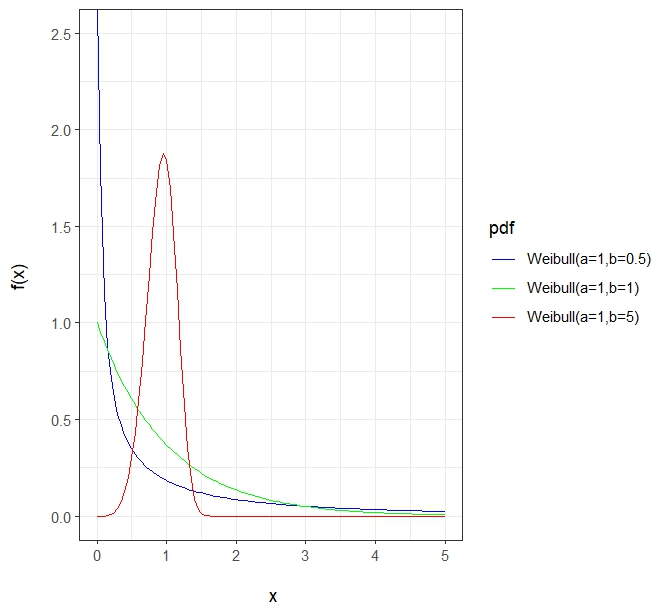
\includegraphics[scale=1]{Figuras/Weibulls.jpeg}
\caption{Distribuciones Weibulls.}
\end{figure}

\begin{theorem}
Si $X$ tiene distribución $Weibull(a,b)$, entonces
\begin{eqnarray*}
E(X) &=&\left( \frac{1}{a}\right) ^{1/b}\Gamma \left( 1+\frac{1}{b}\right) \\
V(X) &=&\left( \frac{1}{a}\right) ^{2/b}\left[ \Gamma \left( 1+\frac{2}{b}
\right) -\Gamma ^{2}\left( 1+\frac{1}{b}\right) \right]
\end{eqnarray*}
\end{theorem}

Observación: La fgm solo existe para $b\geq 1$.
Calculo de la esperanza de $X$: 
\begin{equation*}
E(X)=\int_{0}^{\infty }xabx^{b-1}e^{-ax^{b}}dx
\end{equation*}

Sea
\begin{enumerate}
\item[1)] $u=ax^{b}$, \ 
\item[2)] Despejando para $x$ de 1):\ $x=\left( \frac{u}{a}\right) ^{1/b}$
\item[3)] Derivando 1) con respecto de $x:$ $\ du=abx^{b-1}dx$
\end{enumerate}

Entonces
\begin{eqnarray*}
E(X) &=&\int_{0}^{\infty }\left( \frac{u}{a}\right) ^{1/b}e^{-u}du \\
&=&\left( \frac{1}{a}\right) ^{1/b}\int_{0}^{\infty }u^{1/b}e^{-u}du \\
&=&\left( \frac{1}{a}\right) ^{1/b}\int_{0}^{\infty }u^{(1/b+1)-1}e^{-u}du
\text{ \ \ //}\Gamma (t)=\int_{0}^{\infty }x^{t-1}e^{-x}dx \\
&=&\left( \frac{1}{a}\right) ^{1/b}\Gamma \left( \frac{1}{b}+1\right)
\end{eqnarray*}

Luego 
\begin{equation*}
E(X)=\left( \frac{1}{a}\right) ^{1/b}\Gamma \left( \frac{1}{b}+1\right)
\end{equation*}

Por otra parte,
\begin{equation*}
E(X^{2})=\int_{0}^{\infty }x^{2}abx^{b-1}e^{-ax^{b}}dx
\end{equation*}

Considerando el siguiente cambio de variable:
\begin{enumerate}
\item[1)] $u=ax^{b}$

\item[2)] Despejando para $x$ de 1): $x=\left( \frac{u}{a}\right) ^{1/b}$

\item[3)] Derivando 1) con respecto de $x:$ $du=abx^{b-1}dx$
\end{enumerate}


Entonces 
\begin{eqnarray*}
E(X^{2}) &=&\int_{0}^{\infty }x^{2}abx^{b-1}e^{-ax^{b}}dx \\
&=&\int_{0}^{\infty }\left( \frac{u}{a}\right) ^{2/b}e^{-u}du \\
&=&\left( \frac{1}{a}\right) ^{2/b}\int_{0}^{\infty }u^{(2/b+1)-1}e^{-u}du
\text{ \ \ \ //}\Gamma (t)=\int_{0}^{\infty }x^{t-1}e^{-x}dx \\
E(X^{2}) &=&\left( \frac{1}{a}\right) ^{2/b}\Gamma \left( \frac{2}{b}
+1\right)
\end{eqnarray*}

Luego 
\begin{eqnarray*}
V(X) &=&\left( \frac{1}{a}\right) ^{2/b}\Gamma \left( \frac{2}{b}+1\right)
-\left( \frac{1}{a}\right) ^{2/b}\Gamma ^{2}\left( \frac{1}{b}+1\right) \\
&=&\left( \frac{1}{a}\right) ^{2/b}\left[ \Gamma \left( \frac{2}{b}+1\right)
-\Gamma ^{2}\left( \frac{1}{b}+1\right) \right]
\end{eqnarray*}

Para conocer más sobre la distribución Weibull ver Rinne ($2008$) y el Capítulo 21 del Johnson \& Balakrishnan ($1994$).


%%%%%%%%%%%%%%%%%%%%%%%%%%%%%%%%%%%%%%%%%%%%
\subsection{*Logística}


\begin{definition}
 Una v.a $X$ tiene distribución logística($\alpha ,\beta $) si su pdf está dada por 
\begin{equation*}
f(x;\alpha ,\beta )=\frac{1}{\beta }\frac{\exp \left( \frac{-(x-\alpha )}{
\beta }\right) }{\left[ 1+\exp \left( \frac{-(x-\alpha )}{\beta }\right) 
\right] ^{2}}I_{(-\infty ,\infty )}(x)\text{ }
\end{equation*}%
$-\infty <\alpha <\infty $, $\beta >0$. // $X\sim $logística($\alpha
,\beta $)
\end{definition}


\begin{theorem}
Si $X$ tiene distribución logística($\alpha,\beta $), entonces
\begin{eqnarray*}
E(X) &=&\alpha \\
V(X) &=&\frac{\pi ^{2}\beta ^{2}}{3} \\
m_{X}(t) &=&e^{\alpha t}\pi \beta t\csc \left( \pi \beta t\right) .
\end{eqnarray*}    
\end{theorem}


Observación: Si la v.a $X$ tiene distribución logística,
entonces es simétrica respecto a $\alpha $.

\textbf{Demostración}:
Note que 
\begin{equation*}
E(X)=\int_{-\infty }^{\infty }\frac{x}{\beta }\frac{e^{-\left( \frac{
x-\alpha }{\beta }\right) }}{\left[ 1+\exp \left( -\frac{(x-\alpha )}{\beta }
\right) \right] ^{2}}dx
\end{equation*}

Considerando:
\begin{enumerate}
\item[1)] $y=\frac{x-\alpha }{\beta }$
\item[2)] Despejando para $x$ de 1): $x=\beta y+\alpha .$
\item[3)] Derivando 1) con respecto a $x$: $dy=\frac{dx}{\beta }$.
\end{enumerate}

\begin{eqnarray*}
E(X) &=&\int_{-\infty }^{\infty }(\alpha +\beta y)\frac{e^{-y}}{\left[
1+e^{-y}\right] ^{2}}dy \\
&=&\alpha \int_{-\infty }^{\infty }\frac{e^{-y}}{\left[ 1+e^{-y}\right] ^{2}}
dy+\beta \int_{-\infty }^{\infty }y\frac{e^{-y}}{\left[ 1+e^{-y}\right] ^{2}}
dy \\
&=&\alpha \int_{-\infty }^{\infty }\frac{1}{\beta }\frac{\exp \left( -\frac{
x-\alpha }{\beta }\right) }{\left[ 1+\exp \left( \frac{-(x-\alpha )}{\beta }
\right) \right] ^{2}}dx+\beta \int_{-\infty }^{\infty }y\frac{e^{-y}}{\left[
1+e^{-y}\right] ^{2}}dy\text{ //}X\sim \text{logística(}\alpha ,\beta 
\text{)} \\
&=&\alpha \cdot 1+\beta \int_{-\infty }^{\infty }y\frac{e^{-y}}{\left[
1+e^{-y}\right] ^{2}}dy
\end{eqnarray*}


Para la segunda integral se considera:

\begin{description}
\item[1)] $z=\frac{1}{1+e^{-y}}$,

\item[2)] Derivando $1$) con respecto de $y:$ $dz=\frac{e^{-y}}{\left(
1+e^{-y}\right) ^{2}}dy$ \ 

\item[3)] Despejando\ para $y$ de 1) y tomando el logaritmo se tiene: $y=\ln
\left( \frac{z}{1-z}\right) $
\end{description}

Entonces 
\begin{eqnarray*}
\beta \int_{-\infty }^{\infty }y\frac{e^{-y}}{\left[ 1+e^{-y}\right] ^{2}}dy
&=&\beta \int_{0}^{1}\ln \left( \frac{z}{1-z}\right) dz \\
&=&\beta \int_{0}^{1}\ln \left( z\right) dz-\beta \int_{0}^{1}\ln \left(
1-z\right) dz\text{ //Propiedad} \\
&=&\beta \int_{0}^{1}\ln \left( z\right) dz-\beta \int_{0}^{1}\ln \left(
t\right) dt\text{ \ //}t=1-z \\
&=&\beta \ast 0-\beta \ast 0 \\
&=&0
\end{eqnarray*}

Luego
\begin{eqnarray*}
E(X) &=&\alpha +\beta \int_{-\infty }^{\infty }y\frac{e^{-y}}{\left[ 1+e^{-y}
\right] ^{2}}dy \\
&=&\alpha +0 \\
&=&\alpha
\end{eqnarray*}%
Por lo tanto 
\begin{equation*}
E(X)=\alpha .
\end{equation*}


Por otra parte,
\begin{equation*}
E(X^{2})=\int_{-\infty }^{\infty }\frac{x^{2}}{\beta }\frac{e^{-\left( \frac{
x-\alpha }{\beta }\right) }}{\left[ 1+\exp \left( -\frac{(x-\alpha )}{\beta }
\right) \right] ^{2}}dx
\end{equation*}

\textbf{Tarea}. Probar que 
\begin{equation*}
V(X)=\frac{\pi ^{2}\beta ^{2}}{3}
\end{equation*}

%%%%%%%%%%%%%%%%%%%%%%%%%%%%%%%%%%%%
\subsection{*Pareto}

\begin{definition}
Una v.a $X$ tiene distribución Pareto si su pdf está dada por
\begin{eqnarray*}
f(x,x_{0},\theta ) &=&\frac{\theta }{x_{0}}\left( \frac{x_{0}}{x}\right)
^{\theta +1}I_{(x_{0},\infty )}(x) \\
&=&\frac{\theta x_{0}^{\theta }}{x^{\theta +1}}I_{(x_{0},\infty )}(x)
\end{eqnarray*}%
donde $\theta >0$ y $x_{0}>0$. //$X\sim Pareto(x_{0},\theta )$
\end{definition}

\begin{theorem}
Si $X$ tiene distribución $Pareto(x_{0},\theta )$, entonces
\begin{equation*}
\begin{array}{l}
E(X)=\frac{\theta x_{0}}{\theta -1},\text{ \ }\theta >1 \\ 
\\ 
V(X)=\frac{\theta x_{0}^{2}}{\theta -2}-\left( \frac{\theta x_{0}}{\theta -1}
\right) ^{2}\text{, }\theta >2 \\ 
\\ 
\text{La fgm no existe.}
\end{array}
\end{equation*}
\end{theorem}

Demostración
\begin{eqnarray*}
E(X^{k}) &=&\int_{x_{0}}^{\infty }x^{k}\frac{\theta }{x_{0}}\frac{
x_{0}^{\theta +1}}{x^{\theta +1}}dx \\
&=&\theta x_{0}^{\theta +1}\int_{x_{0}}^{\infty }x^{k}\frac{1}{x_{0}}\frac{1
}{x^{\theta +1}}dx \\
&=&\theta x_{0}^{\theta +1}\int_{x_{0}}^{\infty }\frac{1}{x_{0}}\frac{1}{
x^{\theta -k+1}}dx \\
&=&\frac{\theta x_{0}^{\theta +1}}{x_{0}^{\theta -k+1}(\theta -k)}
\int_{x_{0}}^{\infty }\frac{(\theta -k)}{x_{0}}\frac{x_{0}^{\theta -k+1}}{
x^{\theta -k+1}}dx\text{ //}pdf\text{ pareto} \\
&=&\frac{\theta x_{0}^{\theta +1}}{x_{0}^{\theta -k+1}(\theta -k)}
\int_{x_{0}}^{\infty }\frac{(\theta -k)}{x_{0}}\left( \frac{x_{0}}{x}\right)
^{(\theta -k)+1}dx\text{ //}pdf\text{ pareto} \\
&=&\frac{\theta x_{0}^{\theta +1}}{x_{0}^{\theta -k+1}(\theta -k)} \\
&=&\frac{\theta x_{0}^{k}}{\theta -k}
\end{eqnarray*}%
i.e,
\begin{equation*}
E(X^{k})=\frac{\theta x_{0}^{k}}{\theta -k}
\end{equation*}

Para $k=1$
\begin{equation*}
E(X)=\frac{\theta x_{0}}{\theta -1},\text{ }\theta >1\text{\ }
\end{equation*}

Para $k=2$,
\begin{equation*}
E(X^{2})=\frac{\theta x_{0}^{2}}{\theta -2}\text{, }\theta >2
\end{equation*}%
Entonces
\begin{eqnarray*}
V(X) &=&E(X^{2})-(E(X))^{2} \\
&=&\frac{\theta x_{0}^{2}}{\theta -2}-\left( \frac{\theta x_{0}}{\theta -1}
\right) ^{2}\text{, \ }\theta >2
\end{eqnarray*}

%%%%%%%%%%%%%%%%%%%%%%%%%%%%%%%%%%%%%%%%%%
\subsection{t de Student}

\begin{definition}
Una v.a $X$ tiene distribución t de Studen con $v$ grados de libertad, si su pdf está dada por
\begin{equation*}
f(x;v)=\frac{\Gamma \left( \frac{v+1}{2}\right) }{\Gamma \left( \frac{v}{2}
\right) \sqrt{v\pi }}\left( 1+\frac{x^{2}}{v}\right) ^{-\left( \frac{v+1}{2}
\right) }I_{(-\infty ,\infty )}(x)
\end{equation*}%
con $v>0$ // $X\sim t(v)$.
\end{definition}

\begin{figure}[h!]
\centering
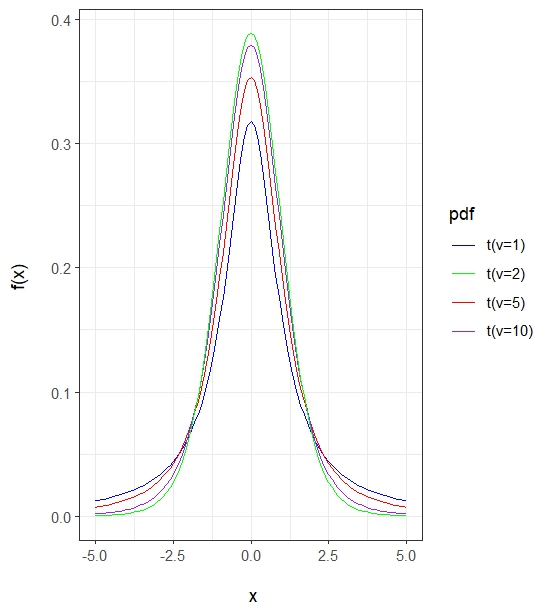
\includegraphics[scale=1]{Figuras/t_students.jpeg}
\caption{Distribuciones t de Student.}
\end{figure}

\begin{theorem}
Si $X$ tiene distribución $t(v)$, entonces
\begin{equation*}
\begin{array}{l}
E(X)=0\text{, \ }v>1 \\ 
\\ 
V(X)=\frac{v}{v-2},\text{ }v>2 \\ 
\\ 
\text{La fgm no existe.}
\end{array}
\end{equation*}
\end{theorem}


Dado que la $t$ de Student es simétrica respecto al origen, entonces
\begin{equation*}
E(X)=0
\end{equation*}


Por otra parte,
\begin{eqnarray*}
E(X^{2}) &=&\int_{-\infty }^{\infty }x^{2}\frac{\Gamma \left( \frac{v+1}{2}
\right) }{\Gamma \left( \frac{v}{2}\right) \sqrt{v\pi }}\left( 1+\frac{x^{2}
}{v}\right) ^{-\left( \frac{v+1}{2}\right) }dx \\
&=&2\int_{0}^{\infty }x^{2}\frac{\Gamma \left( \frac{v+1}{2}\right) }{\Gamma
\left( \frac{v}{2}\right) \sqrt{v\pi }}\left( 1+\frac{x^{2}}{v}\right)
^{-\left( \frac{v+1}{2}\right) }dx\text{// simetr\'{\i}a de la }t \\
&=&2\frac{\Gamma \left( \frac{v+1}{2}\right) }{\Gamma \left( \frac{v}{2}
\right) \sqrt{v\pi }}\int_{0}^{\infty }x^{2}\left( 1+\frac{x^{2}}{v}\right)
^{-\left( \frac{v+1}{2}\right) }dx\text{ }
\end{eqnarray*}


Cambio de variable:
\begin{enumerate}
\item[1)] Sea $u=\frac{x^{2}}{v}$

\item[2)] Despejado para $x$ de 1): $x=\sqrt{uv}$

\item[3)] De 1) derivar $u$ con respecto de $x$: $du=\frac{2x}{v}dx$,

\item[4)] Despejado para $dx$ en 3): $dx=\frac{du}{2x}v$

\item[5)] Sustituyendo 2) en 4): $dx=\frac{vdu}{2\sqrt{uv}}=\frac{\sqrt{v}du
}{2\sqrt{u}}$
\end{enumerate}

Entonces
\begin{eqnarray*}
E(X^{2}) &=&\frac{2\Gamma \left( \frac{v+1}{2}\right) }{\Gamma \left( \frac{v
}{2}\right) \sqrt{v\pi }}\int_{0}^{\infty }uv\left( 1+u\right) ^{-\left( 
\frac{v+1}{2}\right) }\frac{\sqrt{v}du}{2\sqrt{u}} \\
&=&\frac{2\Gamma \left( \frac{v+1}{2}\right) }{\Gamma \left( \frac{v}{2}
\right) \sqrt{v\pi }}\frac{v^{3/2}}{2}\int_{0}^{\infty }u^{1/2}\left(
1+u\right) ^{-\left( \frac{v+1}{2}\right) }du \\
&=&\frac{2\Gamma \left( \frac{v+1}{2}\right) }{\Gamma \left( \frac{v}{2}
\right) \sqrt{v}\sqrt{\pi }}\frac{v^{3/2}}{2}\int_{0}^{\infty }\frac{u^{1/2}
}{\left( 1+u\right) ^{\left( \frac{v+1}{2}\right) }}du \\
&=&\frac{\Gamma \left( \frac{v+1}{2}\right) }{\Gamma \left( \frac{v}{2}
\right) }\frac{v}{\sqrt{\pi }}\int_{0}^{\infty }\frac{u^{3/2-1}}{\left(
1+u\right) ^{3/2+\left( \frac{v}{2}-1\right) }}du\text{ \ //}B(\alpha,\beta
)=\int_{0}^{\infty }\frac{x^{\alpha -1}}{(1+x)^{\alpha +\beta }}dx \\
&=&\frac{\Gamma \left( \frac{v+1}{2}\right) }{\Gamma \left( \frac{v}{2}
\right) }\frac{v}{\sqrt{\pi }}B\left( 3/2,v/2-1\right)
\end{eqnarray*}

i.e,
\begin{eqnarray*}
E(X^{2}) &=&\frac{\Gamma \left( \frac{v+1}{2}\right) }{\Gamma \left( \frac{v
}{2}\right) }\frac{v}{\sqrt{\pi }}\frac{\Gamma (3/2)\Gamma (v/2-1)}{\Gamma
\left( \frac{v+1}{2}\right) } \\
&=&v\frac{\Gamma (3/2)\Gamma (v/2-1)}{\Gamma \left( v/2\right) \sqrt{\pi }}
\text{ \ \ \ //}\Gamma (3/2)=\frac{\sqrt{\pi }}{2} \\
&=&v\frac{\frac{\sqrt{\pi }}{2}\Gamma (v/2-1)}{\Gamma \left( v/2\right) 
\sqrt{\pi }} \\
&=&\frac{v}{2}\frac{\Gamma (v/2-1)}{\Gamma \left( v/2\right) } \\
&=&\frac{v}{2\left( \frac{v}{2}-1\right) } \\
&=&\frac{v}{v-2}\text{, \ \ \ }v>2.
\end{eqnarray*}

Luego
\begin{equation*}
E(X^{2})=\frac{v}{v-2}\text{, \ \ \ }v>2.
\end{equation*}
Entonces%
\begin{eqnarray*}
V(X) &=&E(X^{2})-\left[ E(X)\right] ^{2} \\
&=&\frac{v}{v-2}-0 \\
&=&\frac{v}{v-2}
\end{eqnarray*}

Por lo tanto 
\begin{equation*}
V(X)=\frac{v}{v-2}
\end{equation*}
para $v>2$.

%%%%%%%%%%%%%%%%%%%%%%%%%%%%%%%%%%%%%%%%%%
\subsection{*F} % Distribuciones de probabilidad

%\chapter{Title chapter 1}


\end{document}
 
\blinddocument
